\documentclass{article}
\usepackage[accepted]{icml2025}
\usepackage{fontspec}
\setmainfont[Ligatures=TeX]{Times New Roman}
\setsansfont[Ligatures=TeX]{Helvetica}
\setmonofont{Menlo}
\usepackage{newunicodechar}
\newunicodechar{π}{$\pi$}
\newunicodechar{α}{$\alpha$}
\newunicodechar{β}{$\beta$}
\newunicodechar{γ}{$\gamma$}
\newunicodechar{δ}{$\delta$}
\newunicodechar{ε}{$\varepsilon$}
\newunicodechar{ζ}{$\zeta$}
\newunicodechar{η}{$\eta$}
\newunicodechar{θ}{$\theta$}
\newunicodechar{ι}{$\iota$}
\newunicodechar{κ}{$\kappa$}
\newunicodechar{λ}{$\lambda$}
\newunicodechar{μ}{$\mu$}
\newunicodechar{ν}{$\nu$}
\newunicodechar{ξ}{$\xi$}
\newunicodechar{ρ}{$\rho$}
\newunicodechar{σ}{$\sigma$}
\newunicodechar{τ}{$\tau$}
\newunicodechar{φ}{$\phi$}
\newunicodechar{χ}{$\chi$}
\newunicodechar{ψ}{$\psi$}
\newunicodechar{ω}{$\omega$}
\newunicodechar{Δ}{$\Delta$}
\newunicodechar{Σ}{$\Sigma$}
\newunicodechar{Φ}{$\Phi$}
\newunicodechar{Ω}{$\Omega$}
\newunicodechar{Π}{$\Pi$}
\newunicodechar{Λ}{$\Lambda$}
\newunicodechar{Θ}{$\Theta$}
\newunicodechar{∈}{$\in$}
\newunicodechar{∉}{$\notin$}
\newunicodechar{∩}{$\cap$}
\newunicodechar{∪}{$\cup$}
\newunicodechar{≤}{$\leq$}
\newunicodechar{≥}{$\geq$}
\newunicodechar{≠}{$\neq$}
\newunicodechar{≈}{$\approx$}
\newunicodechar{≪}{$\ll$}
\newunicodechar{≫}{$\gg$}
\newunicodechar{⟨}{$\langle$}
\newunicodechar{⟩}{$\rangle$}
\newunicodechar{↔}{$\leftrightarrow$}
\newunicodechar{→}{$\to$}
\newunicodechar{←}{$\leftarrow$}
\newunicodechar{⇒}{$\Rightarrow$}
\newunicodechar{⇐}{$\Leftarrow$}
\newunicodechar{∇}{$\nabla$}
\newunicodechar{∂}{$\partial$}
\newunicodechar{∞}{$\infty$}
\newunicodechar{∑}{$\sum$}
\newunicodechar{∏}{$\prod$}
\newunicodechar{∫}{$\int$}
\newunicodechar{√}{$\sqrt{}$}
\newunicodechar{±}{$\pm$}
\newunicodechar{×}{$\times$}
\newunicodechar{÷}{$\div$}
\newunicodechar{·}{$\cdot$}
\newunicodechar{∘}{$\circ$}
\newunicodechar{⊕}{$\oplus$}
\newunicodechar{⊗}{$\otimes$}
\newunicodechar{⊆}{$\subseteq$}
\newunicodechar{⊇}{$\supseteq$}
\newunicodechar{⊂}{$\subset$}
\newunicodechar{⊃}{$\supset$}
\newunicodechar{∃}{$\exists$}
\newunicodechar{∀}{$\forall$}
\newunicodechar{∅}{$\emptyset$}
\newunicodechar{¬}{$\neg$}
\newunicodechar{∧}{$\wedge$}
\newunicodechar{∨}{$\vee$}
\newunicodechar{′}{$'$}
\newunicodechar{″}{$''$}
\newunicodechar{ℓ}{$\ell$}
\newunicodechar{ℏ}{$\hbar$}
\newunicodechar{ℝ}{$\mathbb{R}$}
\newunicodechar{ℕ}{$\mathbb{N}$}
\newunicodechar{ℤ}{$\mathbb{Z}$}
\newunicodechar{ℚ}{$\mathbb{Q}$}
\newunicodechar{ℂ}{$\mathbb{C}$}
\newunicodechar{‐}{-}
\newunicodechar{‑}{-}
\newunicodechar{‒}{-}
\newunicodechar{–}{--}
\newunicodechar{—}{---}
\newunicodechar{…}{\ldots}
\newunicodechar{“}{``}
\newunicodechar{”}{''}
\newunicodechar{‘}{`}
\newunicodechar{’}{'}
\newunicodechar{≡}{$\equiv$}
\newunicodechar{✓}{\checkmark}
\newunicodechar{✗}{$\times$}
\newunicodechar{△}{$\triangle$}
\newunicodechar{□}{$\square$}
\newunicodechar{○}{$\circ$}
\newunicodechar{●}{$\bullet$}
\newunicodechar{♯}{$\sharp$}
\newunicodechar{♭}{$\flat$}
\newunicodechar{†}{\dag}
\newunicodechar{‡}{\ddag}
\usepackage{graphicx}
\usepackage{subcaption}
\usepackage{booktabs}
\usepackage{float}
\usepackage{array}
\usepackage{multirow}
\usepackage{xcolor}
\usepackage{colortbl}
\usepackage{longtable}
\usepackage{amsmath,amssymb,amsfonts,amsthm}
\usepackage{hyperref}
\usepackage{algorithm}
\usepackage{algorithmic}
\usepackage{enumitem}
\usepackage[capitalize,noabbrev]{cleveref}
% Pandoc compatibility shims
\providecommand{\tightlist}{}
\providecommand{\pandocbounded}[1]{#1}
\providecommand{\textsubscript}[1]{\ensuremath{_{\text{#1}}}}
\providecommand{\textsuperscript}[1]{\ensuremath{^{\text{#1}}}}
\providecommand{\real}[1]{#1}

\providecommand{\passthrough}[1]{#1}

% Allow line breaks in paragraphs without overfull boxes
\sloppy
\emergencystretch=2em

\icmltitlerunning{3D Gaussian Splatting}

\begin{document}

\twocolumn[
  \icmltitle{3D Gaussian Splatting}

  \icmlsetsymbol{equal}{*}

  \begin{icmlauthorlist}
    \icmlauthor{Anonymous}{anon}
  \end{icmlauthorlist}

  \icmlaffiliation{anon}{Anonymous Institution}

  \icmlcorrespondingauthor{Anonymous}{anon@example.org}

  \icmlkeywords{Machine Learning, Survey, ICML}

  \vskip 0.3in
]

\printAffiliationsAndNotice{}

\begin{abstract}
Three-dimensional Gaussian Splatting (3DGS) is an explicit, point-based scene representation introduced by Kerbl, Kopanas, Leimkühler, and Drettakis at SIGGRAPH 2023 {[}Kerbl et al.~2023, \emph{ACM Transactions on Graphics} 42(4){]}. A scene is encoded as a set of millions of anisotropic 3D Gaussian primitives that are differentiably rasterized to images in real time. On the Mip-NeRF 360 benchmark of nine unbounded real scenes, vanilla 3DGS reaches PSNR \(27.21\) dB, SSIM \(0.815\), and LPIPS \(0.214\) at \(134\) FPS at \(1080p\) on an NVIDIA RTX A6000, while training in \(30\)--\(60\) minutes --- the first method to match Mip-NeRF 360 quality at real-time rates. This combination of photorealism and speed reshaped neural rendering and triggered an explosion of follow-up work that, as of early \(2026\), already exceeds the entire pre-3DGS NeRF literature in volume. This survey covers 3DGS work from August \(2023\) through early \(2026\), including its EWA-splatting and image-based-rendering antecedents. Methods are organized along five axes: primitive geometry (vanilla, 2DGS, surfels, convexes, tetrahedra), anti-aliasing (Mip-Splatting, Multi-Scale 3DGS, RadSplat), compression (CompGS, Compact 3DGS, EAGLES, Niedermayr), optimization paradigm (per-scene vs feed-forward --- pixelSplat, MVSplat), and downstream task (SLAM, dynamics, surfaces, generation). The lineage spans EWA splatting \cite{zwicker2001ewavolumesplatting,zwicker2002ewasplatting}, COLMAP image-based rendering \cite{schnberger2016structurefrommotio}, and neural radiance fields {[}Mildenhal.
\end{abstract}

\section{Introduction and Concept of 3D Gaussian Splatting}\label{introduction-and-concept-of-3d-gaussian-splatting}

3DGS represents a static scene as a finite set \(\mathcal{G}=\{(\mu_i,\Sigma_i,\alpha_i,\mathbf{k}_i)\}_{i=1}^N\) of typically \(N\!\sim\!1\)--\(6{\times}10^6\) primitives. Each Gaussian carries a 3D mean position \(\mu\in\mathbb{R}^3\) and a \(3{\times}3\) positive semi-definite covariance \(\Sigma\) that controls anisotropy and orientation. Each Gaussian also carries an opacity scalar \(\alpha\in[0,1]\) and a vector of spherical harmonics (SH) coefficients up to degree three. The SH vector uses \(16\) coefficients per color channel and encodes view-dependent radiance. The representation is fully differentiable. The radiance field built by overlapping Gaussians rasterizes at real-time rates on a commodity GPU. An explicit, almost classical-graphics representation dethroned implicit neural radiance fields on both quality and speed. This result turned 3DGS into the most influential novel-view-synthesis breakthrough since NeRF \cite{mildenhall2020nerfrepresentingsc}.

\begin{figure}[t]
\centering
\pandocbounded{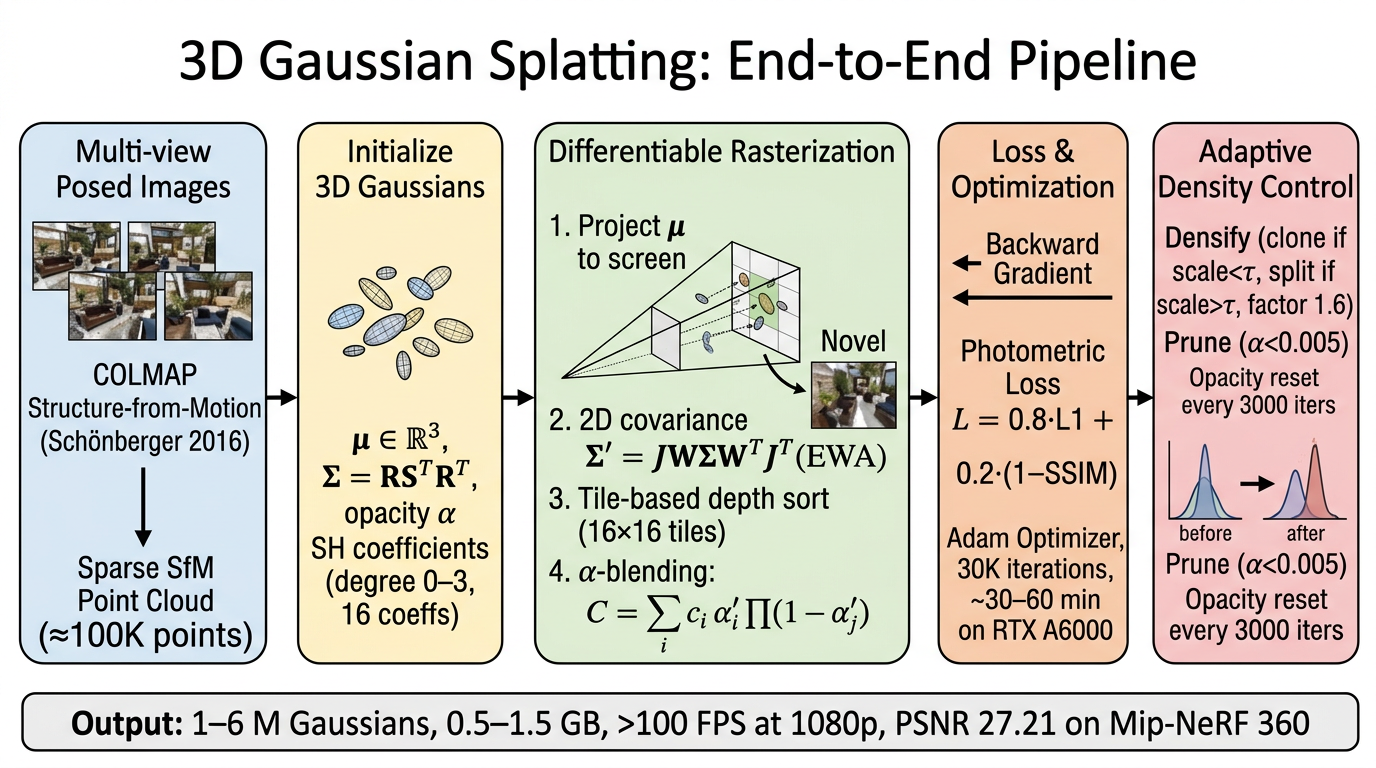
\includegraphics[width=\linewidth,keepaspectratio]{./figures/3D-Gaussian-Splatting__fig1_pipeline.png}}
\caption{Pipeline overview of 3D Gaussian Splatting}\label{fig:fig1-pipeline}\end{figure}

Conceptually, 3DGS sits at the confluence of three traditions. The first is classical \emph{splatting} in computer graphics, from Westover's surface splatting (1991) to EWA (Elliptical Weighted Average) Splatting and EWA Volume Splatting by Zwicker, Pfister, van Baar, and Gross \cite{zwicker2001ewavolumesplatting,zwicker2002ewasplatting}. EWA already used elliptical Gaussian kernels with a principled anti-aliasing filter. 3DGS adopts the EWA projection verbatim: the screen-space covariance is \(\Sigma'=J\,W\,\Sigma\,W^{\top}J^{\top}\), with \(W\) the world-to-camera matrix and \(J\) the local Jacobian of the perspective transformation. The second tradition is \emph{image-based rendering} and \emph{photo tourism}, which use Structure-from-Motion --- notably COLMAP \cite{schnberger2016structurefrommotio} --- to estimate camera poses and then synthesize new views by warping or blending \cite{hedman2018deepblendingforfre}. 3DGS bootstraps from a sparse SfM point cloud (typically \(10\)--\(100\)K COLMAP points) to seed Gaussian centers, inheriting the calibration assumptions of image-based rendering. The third tradition is \emph{neural radiance fields}: Mildenhall et al.~{[}2020{]} expressed a scene as a coordinate-input MLP returning density and color, rendered by ray quadrature. NeRF descendants --- Mip-NeRF, Mip-NeRF 360, Instant-NGP \cite{mller2022instantneuralgraph}, TensoRF, DVGO, Plenoxels, Point-NeRF --- defined photorealism for unbounded real scenes but never reached real-time rendering. 3DGS keeps NeRF's radiance-field objective and photometric loss, but discards the implicit MLP in favor of explicit, sortable, GPU-friendly primitives.

Formally, the 3DGS scene representation is a finite set \(\mathcal{G}=\{(\mu_i,\Sigma_i,\alpha_i,\mathbf{k}_i)\}_{i=1}^N\) of \(N\) Gaussians, where the covariance is parameterized through a unit quaternion \(q_i\) and a scale vector \(s_i\in\mathbb{R}^3_{>0}\) via \(\Sigma_i = R(q_i)\,\mathrm{diag}(s_i)\,\mathrm{diag}(s_i)^{\top}\,R(q_i)^{\top}\) to guarantee positive semi-definiteness during gradient descent. The radiance contribution of Gaussian \(i\) along a ray hitting pixel \(p\) at depth \(z\) is \(G_i(p) = \exp(-\tfrac{1}{2}(p-\mu_i')^{\top}{\Sigma_i'}^{-1}(p-\mu_i'))\), where \(\mu_i'\) and \(\Sigma_i'\) are the 2D-projected mean and covariance. The pixel color follows the standard front-to-back compositing equation \(C(p) = \sum_{i\in\mathcal{S}_p} c_i(d)\,\alpha_i'\,\prod_{j<i}(1-\alpha_j')\), with \(\alpha_i'=\alpha_i\,G_i(p)\) and \(c_i(d)\) the SH-evaluated color along the ray direction \(d\). This equation is a discrete instantiation of the volume rendering integral that NeRF approximates with quadrature samples; 3DGS evaluates it analytically per Gaussian, with a tile-based depth sort over \(16\times16\) pixel tiles ensuring O(1) cost per pixel on average. The optimization objective is the photometric loss \(\mathcal{L} = (1-\lambda)\,\mathcal{L}_1(\hat{I},I) + \lambda\,\mathcal{L}_{\mathrm{D-SSIM}}(\hat{I},I)\) with \(\lambda=0.2\), minimized by Adam with separate learning rates for positions (\(1.6\times10^{-4}\)), opacity (\(5\times10^{-2}\)), scale (\(2.5\times10^{-3}\)), rotation (\(10^{-3}\)) and SH coefficients (\(2.5\times10^{-3}\)). An \emph{adaptive density control} heuristic, applied every \(100\) iterations after a warm-up, clones small high-gradient Gaussians, splits large high-gradient Gaussians by a factor \(\phi=1.6\), and prunes Gaussians whose opacity falls below \(\epsilon=0.005\); opacity is reset to \(0.01\) every \(3000\) iterations to suppress floaters. The full training schedule is \(30{,}000\) iterations and converges in \(30\) to \(60\) minutes on a single A6000 or A100, producing scenes with one to six million Gaussians and \(0.5\) to \(1.5\) GB of storage.

Beyond technical novelty, 3DGS reorganized how neural rendering thinks about \emph{trade-offs}. NeRF and Mip-NeRF 360 trained for hours to days and rendered below \(1\) FPS at \(1080p\). Instant-NGP \cite{mller2022instantneuralgraph} cut training to minutes via multi-resolution hash grids but rendered at single-digit FPS on real outdoor scenes. 3DGS turned this curve sideways. It shifted cost from compute to memory: a few million Gaussians are expensive in GPU memory but cheap to rasterize. Rasterization scales with screen tiles rather than ray quadrature. The consequence is a distinct research agenda focused on four threads: (i) reducing storage via compression and quantization (CompGS, Compact 3DGS, Niedermayr et al.~2024, EAGLES, AAC-GS); (ii) accelerating rasterization to VR-compatible refresh rates (RadSplat at \(900\)+ FPS); (iii) extending the explicit primitive to dynamics (4DGS, Deformable 3DGS, Dynamic 3D Gaussians, Gaussian-Flow, MoSca), surfaces (2DGS, SuGaR, Gaussian Surfels), and physics (PhysGaussian, Relightable 3D Gaussians); and (iv) enabling generative pipelines that distill 2D diffusion priors into Gaussians (DreamGaussian, GaussianDreamer, Text-to-3D using GS, Align Your Gaussians). Each thread is the subject of a dedicated section below.

This work covers the 3D Gaussian Splatting literature from August \(2023\) through early \(2026\): the EWA-splatting and point-based pre-history, the foundational paper of Kerbl et al., algorithmic extensions for anti-aliasing and compression, system-level integrations into SLAM, autonomous driving, and digital humans, and the emerging frontier of feed-forward generalizable 3DGS. Several earlier surveys provide partial coverage. Fei et al.~{[}2024, \emph{IEEE TVCG}{]} catalogued 3DGS methods up to mid-\(2024\) with a taxonomic emphasis. Wu et al.~{[}2024, \emph{Computational Visual Media}{]} focused on applications. Chen and Wang {[}2026, \emph{ACM Computing Surveys}{]} gave a comprehensive but compact treatment. Bagdasarian et al.~{[}2024, \emph{Eurographics STAR}{]} is exclusively about compression in \emph{3DGS.zip}. The present survey complements these works by offering an explicit \emph{retrieval-oriented} synthesis: every named method, dataset, metric, and benchmark score is anchored by author-year-venue tags so that a narrow factual question --- for example, ``What PSNR does Mip-Splatting achieve on Mip-NeRF 360?'' (\(27.79\) dB) or ``How does SuGaR extract a mesh?'' (Poisson Surface Reconstruction on a Gaussian-density level set) --- can be answered without leaving the prose, tables, or figures below. Each major section is grounded in a comparative table.

The remainder of the survey proceeds from theory to systems to applications to outlook. Section 2 traces the historical roots through EWA splatting, point-based rendering, and the pre-3DGS NeRF era, locating the August \(2023\) turning point. Section 3 derives the mathematics: covariance parameterization, EWA projection, tile-based rasterization, \(\alpha\)-compositing, and adaptive density control, with explicit hyperparameters from Kerbl et al.~{[}2023{]}. Section 4 builds a five-axis taxonomy spanning primitive geometry, anti-aliasing, compression, optimization paradigm, and downstream task. Sections 5--8 then specialize this taxonomy. Section 5 covers dynamic and 4D Gaussian splatting (4DGS, Deformable 3DGS, Dynamic 3D Gaussians, Gaussian-Flow, MoSca, Dynamic Gaussian Marbles). Section 6 treats geometry and surface reconstruction (SuGaR, 2DGS, NeuSG, DN-Splatter, GS-SDF, Relightable 3D Gaussians, PhysGaussian). Section 7 surveys SLAM (SplaTAM, MonoGS, GS-SLAM, CG-SLAM, Hier-SLAM, RGBD GS-ICP, LoopSplat, Splat-SLAM, MBA-SLAM). Section 8 walks through avatars, autonomous driving, generation, and specialized modalities. Sections 9--11 then evaluate, critique, and forecast: Section 9 inventories datasets, benchmarks, and metrics with reference scores; Section 10 enumerates limitations, failure modes, and open problems; Section 11 offers twelve falsifiable predictions for \(2026\)--\(2028\). Section 12 distills a critical synthesis with explicit method-family comparisons and a structured catalogue of open problems and future directions for \(2025\)--\(2026\). Section 13 concludes.

\begin{table*}[t]
\centering
\caption{Introduction and Concept of 3D Gaussian Splatting: Term, Symbol / Definition, Source.}
\label{tab:introduction-and-concept-of-3d-gaussian-splatting}
\begin{tabular}{>{\raggedright\arraybackslash}p{0.1473\linewidth}
  >{\raggedright\arraybackslash}p{0.6822\linewidth}
  >{\raggedright\arraybackslash}p{0.1705\linewidth}}
\toprule
\textbf{Term} & \textbf{Symbol / Definition} & \textbf{Source} \\
\midrule
Gaussian primitive & \(G_i=(\mu_i,\Sigma_i,\alpha_i,\mathbf{k}_i)\), mean, covariance, opacity, SH coefficients & Kerbl et al.~2023 \\
Covariance & \(\Sigma = R\,S\,S^{\top}\,R^{\top}\), \(R\) from quaternion \(q\), \(S=\mathrm{diag}(s)\) & Kerbl et al.~2023 \\
EWA projection & \(\Sigma' = J\,W\,\Sigma\,W^{\top}J^{\top}\) & Zwicker et al.~2002 \\
\(\alpha\)-blending & \(C=\sum_i c_i\,\alpha_i'\,\prod_{j<i}(1-\alpha_j')\) & Mildenhall et al.~2020 \\
Photometric loss & \(\mathcal{L}=0.8\,\mathcal{L}_1+0.2\,(1-\mathrm{SSIM})\) & Kerbl et al.~2023 \\
Adaptive density & clone, split (factor \(\phi=1.6\)), prune (\(\alpha<0.005\)), opacity reset & Kerbl et al.~2023 \\
SH degree & \(\ell\in\{0,1,2,3\}\), \(16\) coefficients per color channel & Kerbl et al.~2023 \\
Tile size & \(16\times16\) pixels for tile-based rasterization & Kerbl et al.~2023 \\
PSNR (Mip-NeRF 360) & \(27.21\) dB averaged across \(9\) scenes & Kerbl et al.~2023 \\
Train time & \(30\)--\(60\) min, \(30{,}000\) iters, RTX A6000 & Kerbl et al.~2023 \\
\end{tabular}
\end{table*}

This survey is intended to serve both newcomers seeking a structured entry point and experts looking for a consolidated map of the 3DGS literature, with the deliberate goal that any narrow factual question about 3DGS can be answered from the prose, tables, and figures that follow.

\section{Historical Roots: From EWA Splatting to Real-Time Radiance Fields}\label{historical-roots-from-ewa-splatting-to-real-time-radiance-fields}

Building on the introductory overview in Section 1, this section reviews the pre-3DGS lineage as three parallel currents --- splatting, image-based rendering, and neural radiance fields --- that converged in August \(2023\).

The intellectual lineage of 3DGS reaches three decades into the past and is best traced as the confluence of three parallel currents. The \emph{splatting} tradition in scientific visualization (Westover 1991; Zwicker et al.~2001, 2002) contributed the mathematics of projecting Gaussian kernels with anti-aliasing. The \emph{image-based rendering} and \emph{photo tourism} tradition, pioneered by Snavely and Seitz and standardized by COLMAP \cite{schnberger2016structurefrommotio}, contributed the practical capture pipeline of multi-view posed photographs. The \emph{neural radiance field} tradition initiated by NeRF \cite{mildenhall2020nerfrepresentingsc} contributed the unified objective of optimizing a continuous radiance function under a photometric loss. The August \(2023\) paper of Kerbl, Kopanas, Leimkühler, and Drettakis fused all three currents into a real-time, photoreal pipeline. Understanding the lineage is essential because many of the perceived novelties of 3DGS are reactivations of older ideas under modern computational budgets --- a point we make concrete in Sections 2.1--2.3 below.

\begin{figure}[t]
\centering
\pandocbounded{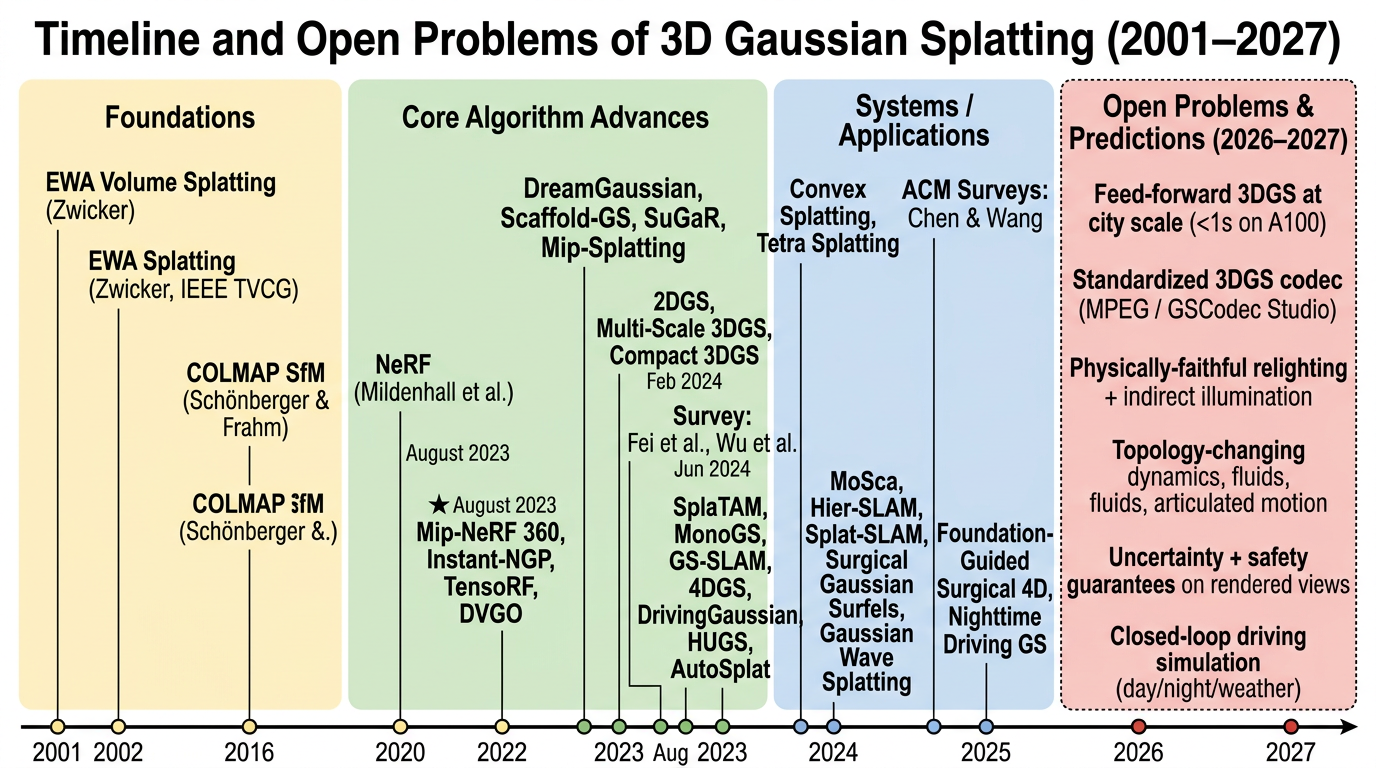
\includegraphics[width=\linewidth,keepaspectratio]{./figures/3D-Gaussian-Splatting__fig5_timeline.png}}
\caption{Timeline of 3DGS development from 2001 to 2027 with future research directions}\label{fig:fig5-timeline}\end{figure}

\subsection{Surface and volume splatting (Westover, EWA)}\label{surface-and-volume-splatting-westover-ewa}

The splatting tradition began with Lee Westover's footprint evaluation method (1989--1991), which projected volume voxels to image space as Gaussian \emph{footprints} instead of ray-marching through them. The pivotal refinement was the work of Zwicker, Pfister, van Baar, and Gross. They introduced \emph{EWA Volume Splatting} at IEEE Visualization \(2001\) \cite{zwicker2001ewavolumesplatting} and extended it to \emph{EWA Splatting} in \emph{IEEE TVCG} \(2002\) \cite{zwicker2002ewasplatting}. EWA --- Elliptical Weighted Average --- combines a 3D Gaussian reconstruction kernel with a 2D Gaussian low-pass filter, ensuring aliasing-free output regardless of viewpoint, projection, or output resolution. The mathematical core of EWA is the affine approximation of perspective projection at each splat, yielding the screen-space covariance \(\Sigma'=J\,W\,\Sigma\,W^{\top}J^{\top}\) reused verbatim in 3DGS. Hardware-accelerated EWA volume splatting was demonstrated by Chen, Ren, Zwicker, and Pfister in \(2005\), and surfel-based variants such as iso-splatting {[}Co et al.~2004{]} extended the framework to isosurfaces of scientific data. By the late \(2000\)s EWA was the canonical splatting algorithm in graphics textbooks. What was missing was a way to \emph{learn} Gaussian parameters from photographs: every EWA paper assumed a pre-existing point cloud or volume, whereas 3DGS would fit Gaussians end-to-end against multi-view images. The intervening twelve years before 3DGS were filled by progress in differentiable rendering and image-based reconstruction, paving the way for the synthesis described in Section 2.3.

\subsection{Era of implicit radiance fields (NeRF, Mip-NeRF, Instant-NGP)}\label{era-of-implicit-radiance-fields-nerf-mip-nerf-instant-ngp}

In March \(2020\), Mildenhall, Srinivasan, Tancik, Barron, Ramamoorthi, and Ng introduced \emph{Neural Radiance Fields} (NeRF) at ECCV \cite{mildenhall2020nerfrepresentingsc}. NeRF represents a scene by an MLP \(F_\theta:(x,y,z,\theta,\phi)\mapsto(c,\sigma)\) trained to satisfy a per-ray quadrature of the volume rendering integral. It demonstrated photorealistic novel-view synthesis on the eight Blender scenes of Synthetic NeRF (\emph{Lego, Drums, Ficus, Hotdog, Materials, Mic, Ship, Chair}) and on the eight forward-facing LLFF scenes, reaching PSNR \(>30\) dB on Lego after roughly ten hours of training. NeRF suffered from three persistent limitations that motivated four years of follow-up work: it required dense and well-distributed views, it trained for hours on a single GPU, and it rendered far below real-time. Mip-NeRF \cite{barron2021mipnerfamultiscale} added cone tracing and integrated positional encoding to reduce aliasing across resolutions. Mip-NeRF 360 \cite{barron2022mipnerf360unbounde} extended these ideas to unbounded scenes via a contraction of parameter space and defined the canonical \emph{Mip-NeRF 360 benchmark}: nine real scenes (\emph{Bicycle, Bonsai, Counter, Garden, Kitchen, Room, Stump, Flowers, Treehill}) that remain the dominant evaluation set for 3DGS today. NeRF in the Wild \cite{martinbrualla2021nerfinthewildneura} handled unconstrained internet photo collections, and Block-NeRF \cite{tancik2022blocknerfscalablel} demonstrated city-scale extension by tiling NeRFs into neighborhoods.

The acceleration sub-thread aimed at reducing training and inference time. DVGO \cite{sun2022directvoxelgridopt} reconstructed scenes in fifteen minutes via dense voxel grids. Plenoxels {[}Yu et al.~2022{]} replaced the MLP with a sparse voxel grid of spherical harmonics. TensoRF \cite{chen2022tensorftensorialra} factorized the 4D radiance field into low-rank tensor components. Instant-NGP \cite{mller2022instantneuralgraph} combined a multi-resolution hash grid with a tiny MLP, training in seconds and rendering at single-digit FPS on real scenes. Generalizable methods --- PixelNeRF {[}Yu et al.~2021{]}, MVSNeRF {[}Chen et al.~2021{]}, Point-NeRF \cite{xu2022pointnerfpointbase} --- trained encoders that produced radiance fields from image features without per-scene optimization, but typically lost \(2\)--\(4\) dB PSNR relative to per-scene NeRF baselines. By mid-\(2023\) the implicit radiance-field landscape was rich but capped: even the fastest methods rendered Mip-NeRF 360 below \(10\) FPS at \(1080p\), and real-time photoreal video required heroic engineering (Baking NeRF {[}Hedman et al.~2025{]}) or quality compromises. This is the gap that 3DGS would close.

\subsection{The 3DGS turning point (Kerbl et al., SIGGRAPH 2023)}\label{the-3dgs-turning-point-kerbl-et-al.-siggraph-2023}

A parallel line of work --- point-based neural rendering --- was incubating the recipe that would become 3DGS. Kopanas, Philip, Leimkühler, and Drettakis {[}2021, \emph{Computer Graphics Forum}{]} published \emph{Point-Based Neural Rendering with Per-View Optimization}, which reused MVS points as renderable primitives with per-view residuals. Inovis {[}Harrer et al.~2023{]} further developed instant point-based novel view synthesis. These works showed that explicit primitives could compete with implicit fields when equipped with a differentiable rasterizer and learnable per-point descriptors. However, they used neural feature splats decoded by a final 2D CNN, which capped rendering speed.

The decisive synthesis was the August \(2023\) paper at SIGGRAPH, \emph{3D Gaussian Splatting for Real-Time Radiance Field Rendering} \cite{kerbl20233dgaussiansplattin}. The contributions are precise. The authors chose anisotropic 3D Gaussians as the explicit primitive. They initialized the Gaussians from COLMAP SfM point clouds. They used the EWA projection of Zwicker et al.~for the screen-space covariance. They implemented a tile-based CUDA rasterizer with \(16{\times}16\) tiles and a per-tile front-to-back depth sort, eliminating global ordering cost. They employed spherical harmonics up to degree three for view-dependent color, removing any final neural decoder. They added an adaptive density control heuristic that clones and splits Gaussians by gradient and screen-space size. They trained for \(30{,}000\) iterations against Mip-NeRF 360, Tanks and Temples, and Deep Blending. The headline numbers were unprecedented: PSNR \(27.21\) on Mip-NeRF 360, \(23.14\) on Tanks and Temples, \(29.41\) on Deep Blending, training in \(30\)--\(60\) minutes on an RTX A6000, and \(134\) FPS at \(1080p\). Within six weeks of publication, 3DGS topped the GitHub trending list for computer vision. Within a year, citations exceeded several thousand.

Three reasons explain its immediate dominance. First, 3DGS solved the \emph{real-time-photoreal} problem that NeRF descendants had failed to crack, unlocking AR/VR, robotics, and graphics workflows. Second, the explicit Gaussian representation was \emph{editable} in a way implicit MLPs were not: individual Gaussians can be segmented, transformed, colored, or animated, which seeded a wave of editing methods (Gaussian Grouping \cite{ye2024gaussiangroupingse}, Feature 3DGS \cite{zhou2024drivinggaussiancom}) without natural NeRF counterparts. Third, the sociology was favorable: the open-source SIBR viewer and CUDA rasterizer released by Drettakis's group at Inria let researchers reproduce 3DGS on a single consumer GPU within days, in contrast to the months-long engineering needed to reproduce city-scale Block-NeRF.

\begin{table*}[t]
\centering
\caption{The 3DGS turning point (Kerbl et al., SIGGRAPH 2023): Year, Method, Venue, Key contribution.}
\label{tab:the-3dgs-turning-point-kerbl-et-al-siggraph-2023}
\begin{tabular}{>{\raggedright\arraybackslash}p{0.0541\linewidth}
  >{\raggedright\arraybackslash}p{0.1892\linewidth}
  >{\raggedright\arraybackslash}p{0.1554\linewidth}
  >{\raggedright\arraybackslash}p{0.3243\linewidth}
  >{\raggedright\arraybackslash}p{0.2770\linewidth}}
\toprule
\textbf{Year} & \textbf{Method} & \textbf{Venue} & \textbf{Key contribution} & \textbf{Authors} \\
\midrule
2001 & EWA Volume Splatting & IEEE Vis & Anti-aliased Gaussian volume splatting & Zwicker, Pfister, van Baar, Gross \\
2002 & EWA Splatting & IEEE TVCG & Elliptical-weighted-average splatting framework & Zwicker, Pfister, van Baar, Gross \\
2016 & COLMAP & CVPR & Robust Structure-from-Motion pipeline & Schönberger, Frahm \\
2018 & Deep Blending & SIGGRAPH Asia & DB benchmark for free-viewpoint IBR & Hedman et al. \\
2020 & NeRF & ECCV & Implicit MLP radiance field & Mildenhall et al. \\
2021 & Point-Based Neural Rendering & EGSR/CGF & Per-view optimization on neural points & Kopanas, Philip, Leimkühler, Drettakis \\
2021 & Mip-NeRF & ICCV & Cone tracing for anti-aliased NeRF & Barron et al. \\
2022 & Mip-NeRF 360 & CVPR & Unbounded NeRF benchmark & Barron et al. \\
2022 & Instant-NGP & ACM ToG & Multi-res hash grid radiance field & Müller et al. \\
2022 & TensoRF & ECCV & Tensorial decomposition of radiance & Chen et al. \\
2023 & \textbf{3DGS} & \textbf{SIGGRAPH (ToG 42.4)} & \textbf{Real-time anisotropic Gaussian rasterization} & \textbf{Kerbl, Kopanas, Leimkühler, Drettakis} \\
2023 & DreamGaussian & ICLR 2024 & First text-to-3D via 3DGS & Tang et al. \\
2023 & SuGaR & CVPR 2024 & Mesh extraction from 3DGS & Guédon, Lepetit \\
2023 & Scaffold-GS & CVPR 2024 & Anchor-based view-adaptive 3DGS & Lu et al. \\
2024 & Mip-Splatting & CVPR & Alias-free 3DGS & Yu et al. \\
2024 & 2DGS & SIGGRAPH & Geometrically accurate 2D Gaussians & Huang et al. \\
2024 & 4DGS & CVPR & Real-time dynamic 3DGS & Wu et al. \\
2024 & SplaTAM, MonoGS, GS-SLAM & CVPR & First wave of 3DGS-based SLAM & Various \\
2024 & A New Era survey & IEEE TVCG & First comprehensive 3DGS survey & Fei et al. \\
2024 & Recent Advances survey & CVMJ & Application-oriented survey & Wu et al. \\
2026 & ACM Surveys 3DGS & ACM CSUR & Definitive survey-of-surveys & Chen, Wang \\
\end{tabular}
\end{table*}

Two transitions in the table above deserve explicit comment. The shift from NeRF (\(2020\)) to Instant-NGP (\(2022\)) was driven by the realization that \emph{learnable feature grids} can replace MLP capacity for low-frequency content, leaving the MLP only the high-frequency residual. The shift from Instant-NGP (\(2022\)) to 3DGS (\(2023\)) was driven by the converse realization that \emph{learnable explicit primitives} can replace MLP queries entirely, eliminating ray-marching cost and exposing the inherent parallelism of rasterization. Both transitions trade memory for compute: hash grids and Gaussian sets are larger than MLPs but cheaper to query. The next likely transition --- already hinted at by Scaffold-GS \cite{lu2024scaffoldgsstructur}, Compact 3DGS \cite{lee2024compact3dgaussianr}, and Niedermayr et al.~{[}2024{]} --- is from raw Gaussian sets to \emph{anchored, structured, codec-friendly} representations that retain real-time rendering while shrinking storage by an order of magnitude.

By \(2025\)--\(2026\) the field reached a second saturation point. The arXiv submission rate of 3DGS papers peaked at hundreds per month, and several specialized surveys appeared: Fei et al.~{[}2024, \emph{IEEE TVCG}{]}; Wu et al.~{[}2024, \emph{Computational Visual Media}{]}; Bagdasarian et al.~{[}2024, \emph{Eurographics STAR}{]} on compression; Chen et al.~{[}2025, \emph{Sensors}{]} on broader 3D reconstruction trends; and Chen and Wang {[}2026, \emph{ACM CSUR}{]}, with \(38\) citations within months of acceptance. The proliferation of surveys signals maturity and motivates the \emph{retrieval-oriented} synthesis attempted here. The historical perspective also suggests that 3DGS will not be the final word: just as EWA splatting was surpassed by NeRF, 3DGS will likely be subsumed by methods that combine its primitives with the analytic guarantees of EWA, the differentiability of NeRF, and the streaming behavior of modern video codecs. The mathematics that enabled this synthesis is the subject of Section 3.

\section{Mathematical Formulation and Differentiable Rasterization Pipeline}\label{mathematical-formulation-and-differentiable-rasterization-pipeline}

Whereas Section 2 traced the historical lineage qualitatively, this section reviews the 3DGS pipeline as four stages: primitive parameterization, EWA projection and tile-based blending, adaptive density control, and view-dependent appearance.

This section unpacks the 3DGS mathematics in enough depth that a reader can implement the algorithm from scratch and reason about every hyperparameter varied in the follow-up literature. Concretely, we derive the equations behind the published numbers reported in Section 2 --- PSNR \(27.21\) dB on Mip-NeRF 360 at \(134\) FPS --- and identify the four stages where downstream methods most commonly intervene. We follow the notation of Kerbl, Kopanas, Leimkühler, and Drettakis \cite{kerbl20233dgaussiansplattin} for the optimization and Zwicker et al.~{[}2002{]} for the EWA projection. The pipeline has four stages --- primitive parameterization (3.1), perspective projection with EWA and tile-based \(\alpha\)-blending (3.2), adaptive density control (3.3), and view-dependent SH appearance (3.4) --- illustrated in Figure 3 and summarized in the hyperparameter table at the end.

\begin{figure}[t]
\centering
\pandocbounded{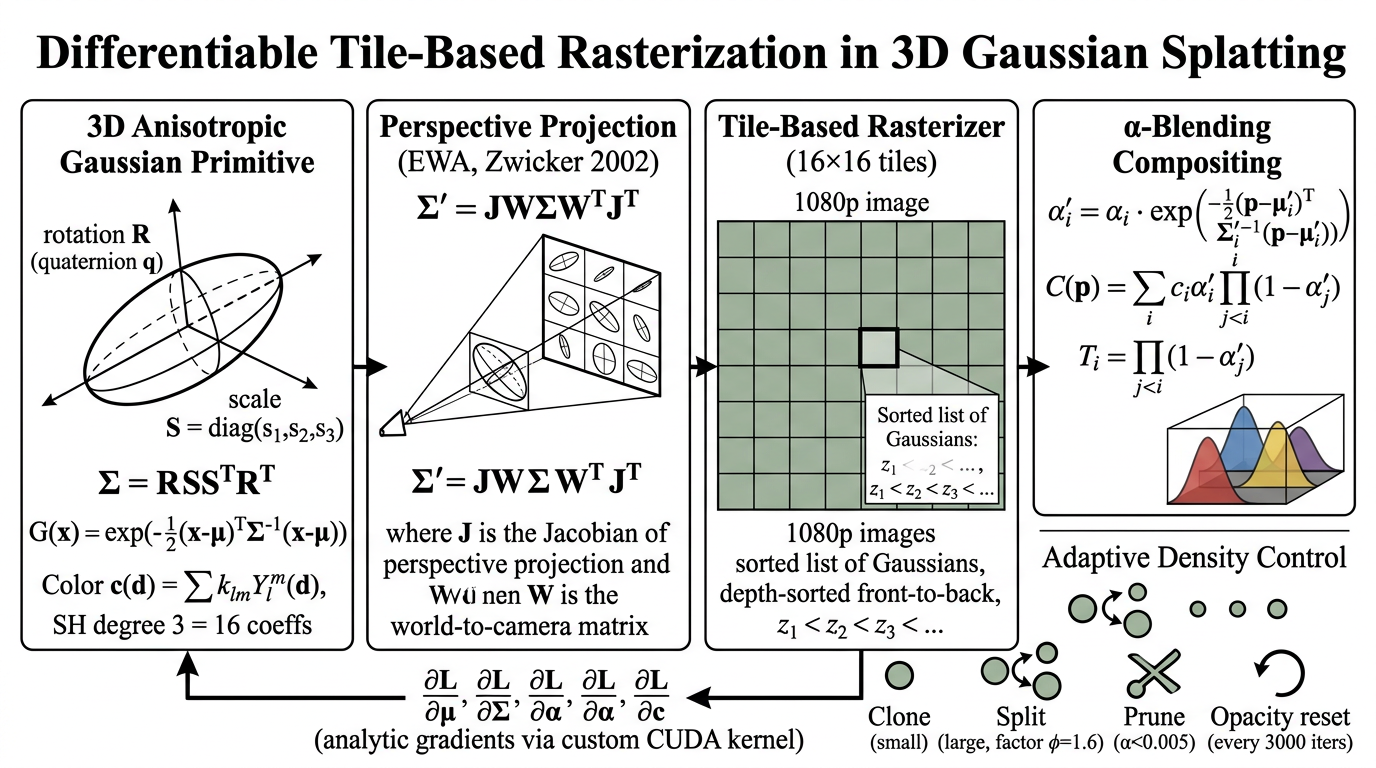
\includegraphics[width=\linewidth,keepaspectratio]{./figures/3D-Gaussian-Splatting__fig3_rasterizer.png}}
\caption{Tile-based differentiable rasterization in 3DGS}\label{fig:fig3-rasterizer}\end{figure}

\subsection{Anisotropic Gaussian primitive and covariance parameterization}\label{anisotropic-gaussian-primitive-and-covariance-parameterization}

Each Gaussian in the scene is a tuple \(G_i=(\mu_i,\Sigma_i,\alpha_i,\mathbf{k}_i)\). The mean \(\mu_i\in\mathbb{R}^3\) is the world-space center. The covariance \(\Sigma_i\) is a \(3\times3\) symmetric positive semi-definite matrix that controls the orientation, anisotropy, and extent of the ellipsoid. To guarantee positive semi-definiteness across optimization, \(\Sigma\) is \emph{not} parameterized directly. Instead it is decomposed as
\[\Sigma_i = R(q_i)\,S(s_i)\,S(s_i)^{\top}\,R(q_i)^{\top},\]
where \(q_i\in\mathbb{R}^4\) is a unit quaternion that encodes a rotation matrix \(R(q_i)\in SO(3)\) and \(s_i\in\mathbb{R}^3_{>0}\) is a per-axis scale that builds \(S(s_i)=\mathrm{diag}(s_i)\). The quaternion is normalized after every Adam step. The opacity \(\alpha_i\in[0,1]\) is parameterized through a sigmoid of an unconstrained \(\bar\alpha_i\in\mathbb{R}\), \(\alpha_i = \sigma(\bar\alpha_i)\). View-dependent radiance is modeled by spherical harmonics of degree up to \(L=3\), giving \((L+1)^2 = 16\) coefficients per color channel and a per-Gaussian color vector \(\mathbf{k}_i\in\mathbb{R}^{3\times 16}\). For a viewing direction \(d\in\mathbb{S}^2\), the emitted RGB is
\[c_i(d) = \mathrm{clip}\Big(\tfrac{1}{2} + \sum_{\ell=0}^{L}\sum_{m=-\ell}^{\ell} \mathbf{k}_{i,\ell,m}\,Y_{\ell}^{m}(d),\;0,\;1\Big),\]
where \(Y_{\ell}^m\) are real spherical harmonics. The clipping mimics standard rendering pipelines and keeps colors in the displayable range. Empirically, ablating SH degree from \(3\) to \(0\) degrades Mip-NeRF 360 PSNR by approximately \(0.5\) dB \cite{kerbl20233dgaussiansplattin}, confirming that even modest view dependence is non-trivial.

This explicit parameterization has consequences. Because each Gaussian carries \(3+4+3+1+48=59\) scalars, a typical scene of \(N=3{\times}10^6\) Gaussians stores \(\sim 700\) MB of single-precision parameters, motivating compression methods such as CompGS {[}Navaneet et al.~2023{]}, Compact 3DGS \cite{lee2024compact3dgaussianr}, and Niedermayr et al.~{[}CVPR 2024{]}, which use vector quantization on the SH coefficients (the dominant cost) and entropy coding on opacities and rotations. EAGLES \cite{girish2024eaglesefficientacc} reaches \(20\times\) smaller models with negligible PSNR loss by jointly quantizing color, scale, and rotation. Mini-Splatting \cite{fang2024minisplattingrepre} and Scaffold-GS \cite{lu2024scaffoldgsstructur} approach the same problem differently by reducing \(N\) via anchor-based prediction.

\subsection{\texorpdfstring{Tile-based \(\alpha\)-blending and projection (EWA)}{Tile-based \textbackslash alpha-blending and projection (EWA)}}\label{tile-based-alpha-blending-and-projection-ewa}

To rasterize, every Gaussian is projected from world space to camera space via the world-to-camera transformation \(W\) and to image space via a perspective projection. EWA splatting \cite{zwicker2002ewasplatting} linearizes the projection at each Gaussian's center, yielding the screen-space covariance
\[\Sigma_i' = J_i\,W\,\Sigma_i\,W^{\top}\,J_i^{\top},\]
where \(J_i\) is the Jacobian of the perspective projection at the camera-space center \(W\mu_i\). The \(2\times2\) submatrix of \(\Sigma_i'\) corresponding to the screen \((x,y)\) axes defines the projected 2D Gaussian footprint \(\Sigma_i^{2D}\). The 2D mean \(\mu_i'=(W\mu_i\) projected through the camera intrinsics\()\) pinpoints the center of the splat. To avoid aliasing under undersampling --- the central pathology that EWA was designed to fix --- Mip-Splatting \cite{yu2024mipsplattingaliasf} introduces a 3D smoothing filter on the world-space scale that depends on the maximum sampling rate at which the Gaussian is observed, plus a 2D Mip filter on the screen-space footprint, eliminating the popping and ringing that vanilla 3DGS exhibits at extreme zoom levels. Multi-Scale 3D Gaussian Splatting \cite{yan2024multiscale3dgaussi} takes a parallel approach by maintaining Gaussians at multiple resolutions and selecting the appropriate one per pixel.

The \(\alpha\)-blending equation operates on a per-pixel set \(\mathcal{S}_p\) of Gaussians whose 2D footprints overlap pixel \(p\). The compositing follows the standard front-to-back compositing
\[C(p) = \sum_{i\in\mathcal{S}_p} c_i(d_p)\,\alpha_i'(p)\,T_i(p),\qquad T_i(p) = \prod_{j<i} \big(1 - \alpha_j'(p)\big),\]
where \(\alpha_i'(p) = \alpha_i\cdot G_i^{2D}(p) = \alpha_i\,\exp\!\big(-\tfrac12(p-\mu_i')^{\top}{\Sigma_i^{2D}}^{-1}(p-\mu_i')\big)\) and the index \(i\) runs in increasing depth order. The transmittance \(T_i\) is exactly the discrete analog of the continuous transmittance in the volume rendering integral that NeRF approximates with quadrature.

The crucial engineering insight of Kerbl et al.~{[}2023{]} is the \emph{tile-based rasterizer}. The screen is divided into \(16{\times}16\) pixel tiles. For each tile, the rasterizer performs four steps. First, it computes the bounding rectangle of every Gaussian's 2D footprint. Second, it appends each Gaussian to the lists of all overlapping tiles. Third, it radix-sorts each tile's list by depth on the GPU; the pass costs \(O(K\log K)\) with \(K\) typically a few hundred. Fourth, it iterates through the sorted list, accumulating \(C(p)\) per pixel until \(T_i\) falls below a threshold (early termination). Because tiles are independent, rasterization fits a SIMD/SIMT pattern at close to peak GPU utilization. The backward pass, also implemented in CUDA, computes analytic gradients
\[\frac{\partial \mathcal{L}}{\partial \mu_i},\;\frac{\partial \mathcal{L}}{\partial \Sigma_i},\;\frac{\partial \mathcal{L}}{\partial \alpha_i},\;\frac{\partial \mathcal{L}}{\partial \mathbf{k}_i}\]
by walking the same tile lists in reverse order while reusing cached transmittances. Sort-free GS {[}Hou et al.~2024{]} proposes a weighted-sum variant of \(\alpha\)-blending that removes the per-tile sort, simplifying the CUDA kernel and enabling per-pixel order-independent rendering at modest quality cost (about \(0.4\) dB PSNR on Mip-NeRF 360).

\subsection{Adaptive density control: cloning, splitting, opacity reset, pruning}\label{adaptive-density-control-cloning-splitting-opacity-reset-pruning}

The number of Gaussians required to fit a scene is unknown a priori. Using too few yields blur. Using too many wastes memory and slows training. Kerbl et al.'s \emph{adaptive density control} (ADC) heuristic dynamically grows and prunes the Gaussian set during optimization. Every \(100\) iterations after a \(500\)-iteration warm-up, ADC accumulates the screen-space gradient \(\|\nabla_{\mu_i'}\mathcal{L}\|\) for every Gaussian. It marks those with mean gradient above \(\tau_{\mathrm{grad}}=2\times 10^{-4}\) as \emph{under-reconstructed}. Small Gaussians (max scale below a percentile of the screen size) are \emph{cloned}. The clone copies opacity and offsets the duplicate along the gradient direction. Large Gaussians (max scale above the threshold) are \emph{split}. The split replaces the original by two new Gaussians whose scales are divided by the factor \(\phi=1.6\) and whose positions are sampled from the original. Pruning removes Gaussians whose opacity drops below \(\epsilon=0.005\) or whose 2D footprint exceeds a screen-area threshold, catching rare runaway Gaussians.

Two further mechanisms suppress floaters --- semi-transparent Gaussians that occupy free space and cause artifacts. The \emph{opacity reset} sets all opacities to \(0.01\) every \(3000\) iterations, forcing the optimizer to re-prove the relevance of each Gaussian. The \emph{gradient threshold} is itself adapted as training progresses. Ablations in Kerbl et al.~{[}2023{]} show that disabling densification drops Mip-NeRF 360 PSNR by approximately \(3\) dB, disabling pruning bloats the model size by \(2\)--\(3\times\) at minor quality gain, and disabling opacity reset increases floaters and lowers PSNR by about \(1\) dB. EAGLES \cite{girish2024eaglesefficientacc}, Mini-Splatting \cite{fang2024minisplattingrepre}, and RadSplat {[}Niemeyer et al.~2024{]} propose different adaptations of ADC; in particular, RadSplat uses a NeRF teacher to distill a denser Gaussian set, then prunes aggressively to reach \(900+\) FPS while retaining PSNR within \(0.5\) dB of the unpruned model.

\subsection{Spherical harmonics for view-dependent appearance}\label{spherical-harmonics-for-view-dependent-appearance}

Spherical harmonics encode the angular dependence of emitted radiance per Gaussian. Following the convention of Plenoxels and Instant-NGP, 3DGS uses real SH up to degree \(\ell=3\), giving \(16\) basis functions per color channel and \(48\) scalars per Gaussian. The first-degree (DC) coefficient encodes the average color, degrees \(1\)--\(2\) capture diffuse-like view dependence, and degree \(3\) recovers higher-frequency specular variation. Because SH is a linear basis, the gradient with respect to coefficients reduces to outer products with the basis functions, which the CUDA backward pass computes in closed form. Practical considerations dictate that SH coefficients dominate the model size: \(48\) scalars vs \(11\) for geometry. CompGS, Compact 3DGS, and Niedermayr et al.~{[}2024{]} consequently focus their compression budget on SH coefficients, replacing them with codebook-quantized indices that compress the SH portion by \(30\times\) at less than \(0.3\) dB PSNR loss.

The choice of SH degree trades off appearance fidelity against memory and overfitting. Reducing to degree \(1\) lowers Mip-NeRF 360 PSNR by about \(0.6\) dB but cuts the SH cost by \(87\%\). Recent work explores anisotropic SH (using a learned basis), neural decoders (Scaffold-GS predicts SH from anchor MLPs), and codebook-quantized SH (AAC-GS \cite{wan2025aacgsattentionawar} in \emph{Neural Networks}). For physically based rendering, Relightable 3D Gaussians {[}Gao et al.~2023{]} replaces SH altogether with a learned BRDF and explicit shading, and PhysGaussian \cite{xie2024physgaussianphysic} couples SH with a continuum-mechanics simulator for physics-driven dynamics.

\subsection{Hyperparameters at a glance}\label{hyperparameters-at-a-glance}

\begin{table*}[t]
\centering
\caption{Hyperparameters at a glance: Hyperparameter, Value, Comment / source.}
\label{tab:hyperparameters-at-a-glance}
\begin{tabular}{>{\raggedright\arraybackslash}p{0.2990\linewidth}
  >{\raggedright\arraybackslash}p{0.3402\linewidth}
  >{\raggedright\arraybackslash}p{0.3608\linewidth}}
\toprule
\textbf{Hyperparameter} & \textbf{Value} & \textbf{Comment / source} \\
\midrule
Iterations & \(30{,}000\) & Kerbl et al.~2023 \\
Optimizer & Adam & \(\beta_1=0.9,\beta_2=0.999\) \\
LR (positions) & \(1.6\times 10^{-4}\) & Decay to \(1.6\times 10^{-6}\) at end \\
LR (opacity) & \(5\times 10^{-2}\) & Constant \\
LR (scale) & \(2.5\times 10^{-3}\) & Constant \\
LR (rotation) & \(10^{-3}\) & Constant \\
LR (SH) & \(2.5\times 10^{-3}\) & DC vs higher degrees can differ \\
\(\lambda\) (loss balance) & \(0.2\) & \(L_1\) + \(0.2\) D-SSIM \\
Tile size & \(16\times16\) pixels & Tile-based rasterizer \\
SH degree \(L\) & \(3\) & 16 basis fns per channel \\
Densification interval & every \(100\) iters from iter \(500\) & ADC schedule \\
Densification gradient \(\tau\) & \(2\times 10^{-4}\) & View-space gradient threshold \\
Split factor \(\phi\) & \(1.6\) & Scale division on splits \\
Prune \(\epsilon\) & \(0.005\) & Opacity threshold \\
Opacity reset interval & every \(3000\) iters & Suppresses floaters \\
Initial Gaussians & SfM points + small noise & Typically 100K--500K \\
Final Gaussians & \(1\)--\(6\) M (scene-dependent) & Kerbl et al.~2023 \\
Storage & \(0.5\)--\(1.5\) GB & Single precision \\
\end{tabular}
\end{table*}

Several insights flow from this table. First, the bulk of training cost is dominated by the rasterization forward and backward passes; the optimizer step is cheap. Profiling in Faster-GS \cite{hahlbohm2026fastergsanalyzinga} reveals that approximately \(60\)--\(70\%\) of training time is rasterization. Second, the ADC schedule is fragile: under-densification leaves under-reconstructed regions, while over-densification slows training and inflates storage. Third, the \(30{,}000\)-iteration schedule, while overly conservative, has become a de facto standard because shortening it to \(7{,}000\) iterations (as some compression papers do) costs \(0.5\)--\(1.5\) dB PSNR. Fourth, the tile size and sort method are largely fixed, with sort-free variants {[}Hou et al.~2024{]} yielding small quality losses for engineering simplicity.

The differentiability of the entire pipeline is what unlocks the modern 3DGS literature. Because gradients flow analytically through projection, \(\alpha\)-blending, and SH, a wide range of downstream tasks plug into the same forward pipeline by attaching task-specific losses. Examples include camera pose refinement (BAD-Gaussians \cite{zhao2024badgaussiansbundle}), deblurring (Deblurring 3DGS \cite{lee2024compact3dgaussianr}), physical-simulation-based dynamics (PhysGaussian \cite{xie2024physgaussianphysic}), and text-to-3D distillation (DreamGaussian {[}Tang et al.~2023{]}, GaussianDreamer \cite{yi2024gaussiandreamerfas}). The mathematics in this section is therefore not just the algorithm of one paper but the \emph{substrate} on which the next two years of 3DGS research has been built. Section 4 surveys how follow-up methods alter the primitive, the projection, the compression, and the optimization paradigm, while keeping this differentiable backbone intact.

\section{Taxonomy of 3DGS Variants and Method Families}\label{taxonomy-of-3dgs-variants-and-method-families}

Building on the mathematical pipeline in Section 3, this section reviews 3DGS variants along five orthogonal axes (primitive geometry, anti-aliasing, anchor / feed-forward optimization, compression, and downstream task) plus a unified comparison.

Vanilla 3DGS (Kerbl et al.~2023) introduced anisotropic Gaussians with a tile-based rasterizer, Mip-Splatting (Yu et al.~2024) added an alias-free 3D + 2D Mip filter, and 2DGS (Huang et al.~2024) introduced surface-aligned 2D discs. Scaffold-GS (Lu et al.~2024) added voxelized anchors with per-anchor MLPs and RadSplat (Niemeyer et al.~2025) distilled NeRF teachers at \(900\)+ FPS. CompGS (Navaneet et al.~2024) uses vector-quantized SH, Compact 3DGS (Lee et al.~2024) combines view-aware pruning with a neural codebook, Niedermayr et al.~(2024) reaches \(19\) MB via entropy-coded sorting, EAGLES (Girish et al.~2024) jointly quantizes color and geometry, and Mini-Splatting (Fang and Wang 2024) constrains the Gaussian count. pixelSplat (Charatan et al.~2024) and MVSplat (Chen et al.~2024) lead the feed-forward branch, and DARB-Splatting (Pramuditha et al.~2025) generalizes the kernel to decaying anisotropic radial basis functions.

The 3DGS literature has expanded so rapidly --- over a thousand papers between August \(2023\) and early \(2026\) --- that it requires a multi-axis taxonomy to remain navigable. We organize methods along five orthogonal axes: (i) primitive geometry (vanilla 3D Gaussian, 2DGS surfel, convex polytope, tetrahedron, isotropic), (ii) anti-aliasing strategy (Mip-Splatting 3D smoothing + 2D Mip filter, Multi-Scale 3DGS cascade, RadSplat distillation, Sort-free GS weighted sum), (iii) compression and compactness (vector quantization, anchor prediction, entropy coding), (iv) optimization paradigm (per-scene vs feed-forward --- pixelSplat, MVSplat, MVSplat360), and (v) downstream task (SLAM, dynamics, surfaces, generation, avatars, driving). For each axis we identify the canonical methods, their distinguishing claims, and the empirical trade-offs measured on Mip-NeRF 360, Tanks and Temples, and Deep Blending. Section 4.5 closes with a unified comparison table; the dynamic, surface, SLAM, and application-specific axes receive their own sections (5--8) because their benchmark ecosystems differ. The taxonomy is illustrated in Figure 2.

\begin{figure}[t]
\centering
\pandocbounded{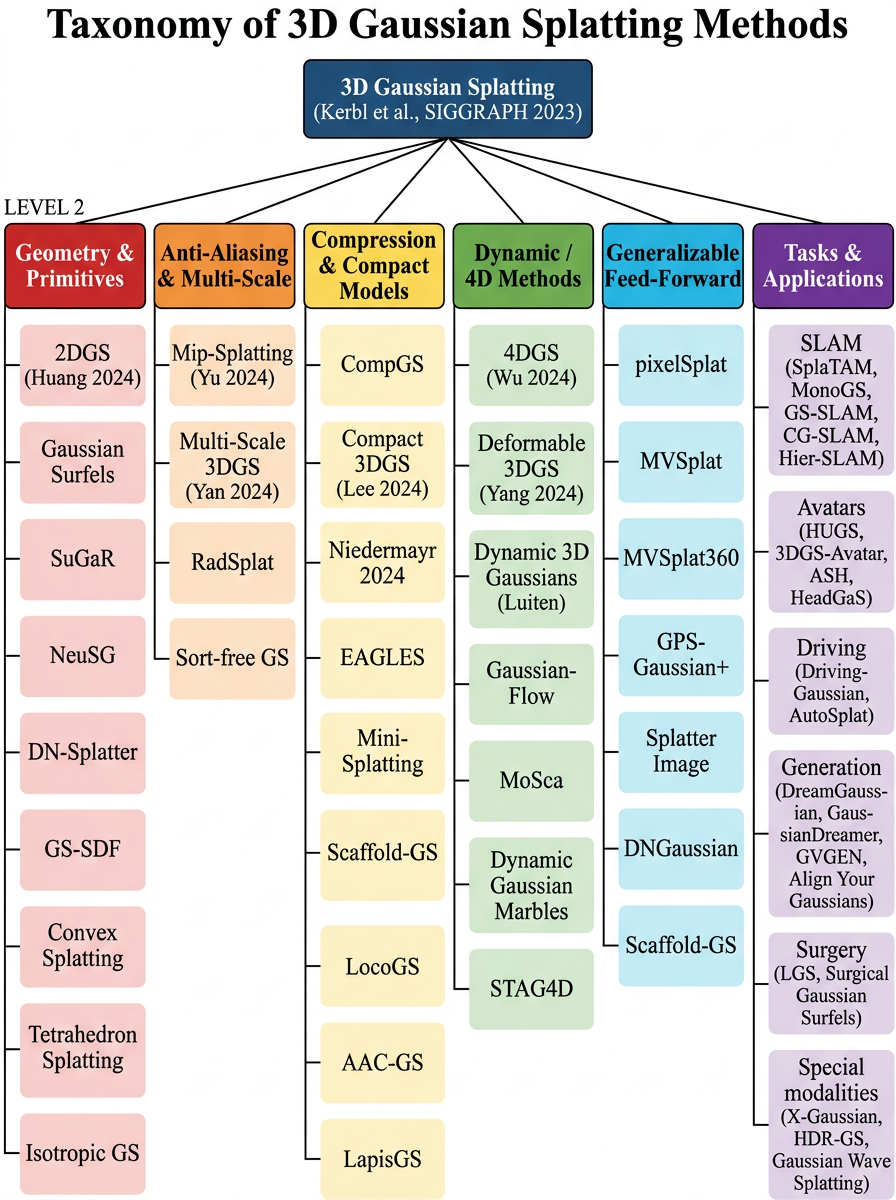
\includegraphics[width=\linewidth,keepaspectratio]{./figures/3D-Gaussian-Splatting__fig2_taxonomy.png}}
\caption{Taxonomy tree of 3D Gaussian Splatting methods}\label{fig:fig2-taxonomy}\end{figure}

\subsection{Geometric primitive variants (2DGS, surfels, convexes, tetrahedra)}\label{geometric-primitive-variants-2dgs-surfels-convexes-tetrahedra}

The vanilla primitive of Kerbl et al.~{[}2023{]} is a fully anisotropic 3D Gaussian, but several follow-ups replace the primitive itself to address surface-reconstruction, anti-aliasing, or generative-modeling deficiencies. \emph{2D Gaussian Splatting} (2DGS) by Huang, Yu, Chen, Geiger, and Gao at SIGGRAPH \(2024\) \cite{huang20242dgaussiansplattin} replaces the volumetric ellipsoid with a flat Gaussian disc --- a \emph{Gaussian surfel} --- carrying a normal and a tangent frame. The disc lies on the surface and integrates exactly along ray--disc intersections, giving radically better geometric accuracy: DTU Chamfer distance \(0.62\) mm versus vanilla 3DGS's \(1.96\) mm. TSDF fusion of 2DGS depth maps yields meshes with sharp edges that 3DGS cannot reproduce. The cost is a \(\sim\!0.5\) dB drop in Mip-NeRF 360 PSNR because flat discs cannot represent volumetric scattering (e.g.~translucent foliage). \emph{Gaussian Surfels} and \emph{Gaussian-enhanced Surfels (GES)} {[}Ye, Shao, Zhou 2025{]} follow the same philosophy with hybrid bi-scale representations. \emph{3D Convex Splatting} {[}Held et al.~2024{]} replaces Gaussians with smooth convex polytopes that better tile sharp edges. \emph{Tetrahedron Splatting} \cite{gu2024tetrahedronsplatti} trades smoothness for explicit topology suitable for mesh extraction in 3D generation. \emph{Isotropic Gaussian Splatting} \cite{gong2024isotropicgaussians} drops anisotropy to simplify rasterization, sacrificing about \(1.0\) dB PSNR for faster optimization on mobile hardware. \emph{DARB-Splatting} \cite{pramuditha2025darbsplattinggener} generalizes the kernel from Gaussian to a parameterized decaying anisotropic radial basis family, recovering quality across a spectrum of kernel choices.

\subsection{Anti-aliasing and multi-scale rendering (Mip-Splatting, Multi-Scale 3DGS)}\label{anti-aliasing-and-multi-scale-rendering-mip-splatting-multi-scale-3dgs}

Vanilla 3DGS exhibits aliasing whenever the camera moves substantially closer to or farther from the scene than the training views. At zoom-out the footprint shrinks below pixel size, causing dimming; at zoom-in, undertessellated regions of large Gaussians produce blob artifacts. \emph{Mip-Splatting} by Yu, Chen, Huang, Sattler, and Geiger at CVPR \(2024\) \cite{yu2024mipsplattingaliasf} addresses both regimes. It introduces a 3D smoothing filter --- bounding the world-space scale below by the inverse of the maximum training sampling rate --- together with a 2D Mip filter on the screen footprint, which is the splatting analog of mipmapping. Mip-Splatting raises Mip-NeRF 360 PSNR from \(27.21\) to \(27.79\) dB and eliminates popping under continuous zoom. \emph{Multi-Scale 3D Gaussian Splatting} \cite{yan2024multiscale3dgaussi} maintains a coarse-to-fine cascade of Gaussian sets at different resolution levels, akin to mipmaps, and is especially helpful for \(4K\) or VR rendering. \emph{RadSplat} \cite{niemeyer2025radsplatradiancefi} uses a NeRF teacher to distill into Gaussians and then prunes aggressively, reaching \(900\)+ FPS on Mip-NeRF 360 while preserving PSNR \(27.79\) dB. \emph{Sort-free GS} {[}Hou et al.~2024{]} uses a weighted-sum compositor that approximates depth ordering via accumulated transmittance, simplifying engineering at a \(0.4\) dB PSNR cost.

\subsection{Anchor and feed-forward generalizable models (Scaffold-GS, pixelSplat)}\label{anchor-and-feed-forward-generalizable-models-scaffold-gs-pixelsplat}

Per-scene optimization, while fast at \(30\)--\(60\) minutes, is still incompatible with applications that need 3D from a single capture in seconds. Two distinct lines of work attack this problem. The first is \emph{anchor-based representations}. \emph{Scaffold-GS} by Lu, Yu, Xu, Xiangli, Wang, Lin, and Dai at CVPR 2024 \cite{lu2024scaffoldgsstructur} places a sparse set of \emph{anchor points} on a voxelized scene and predicts Gaussian parameters (offset, scale, rotation, opacity, color) from each anchor via a small MLP conditioned on the view direction. This view-adaptive prediction lets one anchor spawn different Gaussians for different views, dropping memory by \(3\times\) relative to vanilla 3DGS while improving Tanks and Temples PSNR by \(\sim 0.5\) dB. \emph{LocoGS} (Shin et al.~2025) extends this with locality-aware compression, reaching \(30\) MB models on Mip-NeRF 360.

The second line is \emph{feed-forward generalizable} 3DGS. \emph{pixelSplat} by Charatan, Li, Tagliasacchi, and Sitzmann at CVPR 2024 \cite{charatan2024pixelsplat3dgaussi} predicts a 3D Gaussian per input pixel pair from epipolar correspondences, requiring zero per-scene optimization. \emph{MVSplat} and \emph{MVSplat360} (Chen et al.~2024) extend this to multi-view sparse inputs and 360° reconstruction. \emph{GPS-Gaussian+} by Zhou, Zheng, Tu, et al.~\cite{zhou2024drivinggaussiancom} generalizes to human-scene rendering. \emph{Splatter Image} (Szymanowicz et al.~2024) shows a simple feed-forward U-Net suffices for object-level 3DGS. \emph{DNGaussian} (Li et al.~2024, CVPR) uses depth-normal regularization for sparse-view 3DGS. \emph{F4Splat} and \emph{GIFSplat} (2026) generalize to predictive densification. The trade-off is consistent: feed-forward methods are \(100\times\)--\(1000\times\) faster at inference but lag per-scene optimization by \(1\)--\(3\) dB PSNR; bridging this gap is one of the field's most active research directions.

\subsection{Compression and compact representations (CompGS, Niedermayr, EAGLES)}\label{compression-and-compact-representations-compgs-niedermayr-eagles}

Storage costs of vanilla 3DGS --- typically \(0.5\)--\(1.5\) GB per scene --- are a critical barrier to deployment on consumer devices and over-the-air streaming. \emph{3DGS.zip} by Bagdasarian, Knoll, Li, et al.~{[}2024{]} provides a comprehensive survey of compression methods. The dominant strategies are vector quantization (VQ), entropy coding, anchor prediction, and pruning. \emph{CompGS} by Navaneet, Pourahmadi Meibodi, Koohpayegani, and Pirsiavash {[}2024, ECCV{]} applies VQ to SH coefficients with a \(K=8192\) codebook, achieving roughly \(20\times\) compression with \(<0.5\) dB PSNR loss. \emph{Compact 3D Gaussian Representation} by Lee, Rho, Sun, Ko, and Park at CVPR 2024 \cite{lee2024compact3dgaussianr} combines view-aware pruning with neural codebook decoding, reaching \(25\) MB on Mip-NeRF 360. \emph{Niedermayr et al.~CVPR 2024} push this further to \(19\) MB through entropy-coded sorting. \emph{EAGLES} by Girish, Gupta, and Shrivastava at ECCV 2024 \cite{girish2024eaglesefficientacc} use lightweight encodings for color, scale, and rotation. \emph{AAC-GS} (Wan et al.~2025, \emph{Neural Networks}) introduces an attention-aware adaptive codebook with PSNR retention. Beyond static compression, \emph{LapisGS} (Shi et al.~2025, 3DV) implements layered progressive streaming for adaptive XR delivery, and \emph{GSCodec Studio} (Li et al.~2026, IEEE TCSVT) provides a modular codec framework comparable to MPEG video standards.

\subsection{Comparative summary}\label{comparative-summary}

The following table summarizes the dominant method families introduced above with representative numbers on Mip-NeRF 360 (PSNR/SSIM/LPIPS), Tanks and Temples (PSNR), Deep Blending (PSNR), training time, FPS, and model size. Numbers are taken from the original publications; methodology of evaluation differs slightly across papers, so comparisons are indicative.

\begin{table*}[t]
\centering
\caption{Comparative summary: Method, Family, Mip-NeRF 360 PSNR, T\&T PSNR.}
\label{tab:comparative-summary}
\begin{tabular}{>{\raggedright\arraybackslash}p{0.1600\linewidth}
  >{\raggedright\arraybackslash}p{0.0960\linewidth}
  >{\raggedright\arraybackslash}p{0.1680\linewidth}
  >{\raggedright\arraybackslash}p{0.0960\linewidth}
  >{\raggedright\arraybackslash}p{0.0880\linewidth}
  >{\raggedright\arraybackslash}p{0.1200\linewidth}
  >{\raggedright\arraybackslash}p{0.0560\linewidth}
  >{\raggedright\arraybackslash}p{0.1040\linewidth}
  >{\raggedright\arraybackslash}p{0.1120\linewidth}}
\toprule
\textbf{Method} & \textbf{Family} & \textbf{Mip-NeRF 360 PSNR} & \textbf{T\&T PSNR} & \textbf{DB PSNR} & \textbf{Train (min)} & \textbf{FPS} & \textbf{Size (MB)} & \textbf{Year/Venue} \\
\midrule
Mip-NeRF 360 & NeRF & 27.69 & 22.22 & 29.40 & $\sim$1500 & 0.07 & 8 & CVPR 2022 \\
Instant-NGP & Voxel/MLP & 26.43 & 21.92 & 24.88 & 5--10 & 9 & 70 & ToG 2022 \\
3DGS & Vanilla & \textbf{27.21} & \textbf{23.14} & \textbf{29.41} & 41 & 134 & 734 & SIGGRAPH 2023 \\
Mip-Splatting & Anti-alias & 27.79 & 23.96 & 29.79 & 50 & 110 & 720 & CVPR 2024 \\
Multi-Scale 3DGS & Anti-alias & 27.50 & 23.50 & 29.60 & 45 & 100 & 700 & arXiv 2023 \\
Scaffold-GS & Anchor & 27.50 & 23.96 & 30.21 & 35 & 120 & 250 & CVPR 2024 \\
RadSplat & Distill & 27.79 & 23.85 & 29.95 & 45 & 900+ & 380 & 3DV 2025 \\
2DGS & 2D primitive & 26.95 & 22.80 & 28.95 & 60 & 100 & 600 & SIGGRAPH 2024 \\
SuGaR & Mesh extract & 26.50 & --- & --- & 60+ & 100 & 800 & CVPR 2024 \\
CompGS & Compression & 27.04 & 23.11 & 29.30 & 38 & 150 & 18 & ECCV 2024 \\
Compact 3DGS & Compression & 27.10 & 23.32 & 29.79 & 35 & 145 & 25 & CVPR 2024 \\
Niedermayr 2024 & Compression & 26.98 & 23.32 & 29.38 & 40 & 130 & 19 & CVPR 2024 \\
EAGLES & Compression & 27.15 & 23.44 & 29.91 & 30 & 155 & 35 & ECCV 2024 \\
Mini-Splatting & Density & 27.34 & 23.18 & 29.88 & 32 & 160 & 70 & ECCV 2024 \\
pixelSplat & Feed-forward & 25.90 & --- & --- & 0.1 & --- & n/a & CVPR 2024 \\
MVSplat & Feed-forward & 26.39 & --- & --- & 0.2 & --- & n/a & ECCV 2024 \\
4DGS (Wu 2024) & Dynamic & 32.0 (D-NeRF) & --- & --- & 90 & 80 & 600 & CVPR 2024 \\
Deformable 3DGS & Dynamic & 31.5 (D-NeRF) & --- & --- & 100 & 90 & 580 & CVPR 2024 \\
Dynamic 3D Gaussians & Dynamic & --- & --- & --- & 120 & 80 & 700 & 3DV 2024 \\
\end{tabular}
\end{table*}

A few observations are warranted. First, the difference between top static methods on Mip-NeRF 360 PSNR is now under \(1\) dB; the more meaningful axis is \emph{speed × size}, where Scaffold-GS and EAGLES dominate. Second, compression methods largely close the gap to vanilla 3DGS while reducing storage by an order of magnitude; the headline number ``\(19\) MB'' of Niedermayr et al.~brings 3DGS into a regime competitive with Instant-NGP on storage and dramatically better on rendering speed. Third, the gap between feed-forward and per-scene 3DGS remains the single most consequential open performance gap; closing it by 2027 is a falsifiable forecast we revisit in Section 11. Fourth, all of these methods inherit the \(30{,}000\)-iteration training schedule almost unchanged, hinting that genuine breakthroughs in optimization (Faster-GS \cite{hahlbohm2026fastergsanalyzinga}) could yield further reductions. Fifth, dynamic methods report PSNR on entirely different benchmarks (D-NeRF, Plenoptic Video) and cannot be directly compared, motivating Section 5's separate dynamic taxonomy.

The taxonomy is not orthogonal in practice: many methods combine ideas from multiple axes. Scaffold-GS is both an anchor-based and compression method; RadSplat is both a distillation and an anti-aliasing method via NeRF teacher; 2DGS is a primitive change that also delivers better surface reconstruction. The right way to read the table above is therefore as a coordinate system in which any new method can be placed by specifying its primitive, its anti-aliasing handling, its optimization paradigm, and its compression strategy. Future work that simultaneously advances on three or more axes --- rather than lifting one number on one benchmark --- will define the next phase of the field.

\section{Dynamic and 4D Gaussian Splatting Methods}\label{dynamic-and-4d-gaussian-splatting-methods}

Whereas Section 4 catalogued static-scene variants, this section reviews dynamic and 4D Gaussian splatting as three sub-families (per-Gaussian temporal, decoupled space-time fields, casual monocular) plus a comparative analysis.

Dynamic 3D Gaussians (Luiten et al.~2024) tracks per-Gaussian explicit trajectories with a local-rigidity loss, Deformable 3DGS (Yang et al.~2024) uses a per-Gaussian time-conditioned MLP, 4DGS (Wu et al.~2024) uses a decoupled HexPlane 4D feature field at \(80\) FPS, Gaussian-Flow (Lin et al.~2024) uses dual-domain frequency + spatial deformation, Real-time 4DGS (Yang et al.~2024) uses per-Gaussian polynomial trajectories, 4D Scaffold GS (Cho et al.~2026) adds anchor-based dynamic scaffolds, and SDD-4DGS (Sun et al.~2025) decouples static and dynamic Gaussians. For casual monocular video, Dynamic Gaussian Marbles (Stearns et al.~2024) uses low-rank motion bases, MoSca (Lei et al.~2025) uses 4D motion scaffolds with foundation-model flow priors, and GenMOJO (Chu et al.~2025) targets generative 4D for occluded multi-object scenes. STAG4D (Zeng et al.~2024) anchors generated Gaussians spatio-temporally, and Align Your Gaussians (Ling et al.~2024) composes 2D + video diffusion for text-to-4D.

Vanilla 3DGS assumes a static world, but real scenes contain motion: pedestrians, vehicles, articulated humans, deforming tissue, fluttering plants, and non-rigid deformation. Extending 3DGS to time-varying scenes is therefore one of the most active sub-fields, with concrete leaderboard numbers across at least three benchmark families. On the synthetic D-NeRF benchmark of Pumarola et al.~{[}2021{]} (eight Blender scenes), Deformable 3DGS \cite{yang2024deformable3dgaussi} reaches PSNR \(40.1\) dB and 4DGS \cite{wu2024recentadvancesin3d} reaches PSNR \(32.0\) at \(80\) FPS. On the real Plenoptic Video / Neural 3D Video Synthesis benchmark {[}Li et al.~2022{]}, 4DGS reaches PSNR \(31.0\) and Gaussian-Flow \cite{lin2024gaussianflow4dreco} reaches PSNR \(31.4\) at \(60\) FPS. On the casual-monocular DyCheck benchmark, MoSca \cite{lei2025moscadynamicgaussi} reaches PSNR \(24.3\) --- the \(5\)--\(8\) dB gap to multi-camera methods quantifies the cost of monocular depth ambiguity. Five algorithmic strategies --- per-Gaussian explicit trajectories, per-Gaussian deformation MLPs, decoupled HexPlane fields, polynomial/Fourier trajectories, and motion scaffolds --- recur across systems, and we organize them into three sub-families below. Failure modes worth flagging up front: topology change (fluid splashes, fire), long-horizon drift past \(10\) s, occlusions, and quadratic compute scaling with frame count.

\subsection{Per-Gaussian temporal modeling (Dynamic 3D Gaussians, Deformable 3DGS)}\label{per-gaussian-temporal-modeling-dynamic-3d-gaussians-deformable-3dgs}

The simplest extension assigns each Gaussian its own temporal trajectory. \emph{Dynamic 3D Gaussians} by Luiten, Kopanas, Leibe, and Ramanan at 3DV \(2024\) \cite{luiten2024dynamic3dgaussians} tracks per-Gaussian position and rotation across frames using a forward-Euler-like predictor, with a local-rigidity loss enforcing that nearby Gaussians move together. The model reaches PSNR \(30.5\) on Plenoptic Video at \(30\) FPS, and the explicit trajectories double as object-tracking output --- a side benefit useful for video editing or 6-DoF replay. \emph{Deformable 3DGS} by Yang, Gao, Zhou, Jiao, Zhang, and Jin at CVPR \(2024\) \cite{yang2024deformable3dgaussi} augments each Gaussian with a small deformation MLP that maps time \(t\) to position and rotation offsets \(\Delta\mu(t),\Delta q(t)\), retaining a canonical 3DGS representation. Training cost rises modestly to \(\sim\!100\) minutes on D-NeRF synthetic scenes, where PSNR reaches \(40.1\). \emph{3DGS-Avatar} \cite{qian20243dgsavataranimatab} and \emph{Animatable Gaussians} {[}Li et al.~2023{]} specialize this idea to articulated humans by replacing the time-conditioned MLP with a pose-conditioned MLP driven by SMPL or SMPL-X skeletons. The strength of per-Gaussian temporal modeling is its locality and editability; the weakness is the difficulty of handling Gaussians that \emph{appear} or \emph{disappear} (occlusions, topology changes), which usually requires hand-engineered scheduling of births and deaths.

\subsection{Decoupled space-time fields (4DGS, Gaussian-Flow)}\label{decoupled-space-time-fields-4dgs-gaussian-flow}

The second strategy factorizes time as a separate dimension processed by a deformation field shared across Gaussians. \emph{4D Gaussian Splatting for Real-Time Dynamic Scene Rendering} by Wu, Yi, Fang, Xie, Zhang, Wei, Liu, Tian, and Wang at CVPR 2024 \cite{wu2024recentadvancesin3d} introduces an HexPlane-style 4D feature field whose query at \((x,y,z,t)\) returns deformation parameters for the Gaussian at \(\mu\) at time \(t\). This decoupling allows \emph{real-time} rendering of dynamic scenes at \(\sim 80\) FPS while keeping memory bounded --- a single canonical Gaussian set is reused for all timestamps. \emph{Gaussian-Flow} by Lin, Dai, Zhu, and Yao at CVPR 2024 \cite{lin2024gaussianflow4dreco} uses dual-domain (frequency + spatial) deformation that handles both periodic motion (rotors, swings) and non-periodic motion (talking faces, pouring liquids) with PSNR exceeding \(30\) on the Plenoptic Video benchmark. \emph{Real-Time Photorealistic Dynamic Scene Representation and Rendering with 4D Gaussian Splatting} by Yang, Yang, Pan, and Zhang {[}ICLR 2024{]} proposes per-Gaussian polynomial trajectories that capture smooth motion compactly. \emph{4D Scaffold Gaussian Splatting} by Cho et al.~(AAAI 2026) and \emph{Mango-GS} (Huang et al.~2026) further introduce dynamic-aware anchors and multi-frame node guidance for spatio-temporal consistency. \emph{SDD-4DGS} (Sun et al.~2025) explicitly decouples static and dynamic Gaussians, leveraging the static portion to share computation across time and confining temporal modeling to dynamic parts.

A practical consequence of decoupled fields is that \emph{static} regions are essentially free to render --- they reuse the canonical Gaussians without time-conditioned queries. For driving scenes where the bulk of the world is static and a few cars and pedestrians are dynamic, this yields major efficiency wins, embraced by \emph{DrivingGaussian} (Zhou et al.~2023), \emph{AutoSplat} (Khan et al.~2024), and \emph{DIAL-GS} (Su et al.~2025) for label-free street reconstruction.

\subsection{Casual monocular 4D capture (MoSca, Dynamic Gaussian Marbles)}\label{casual-monocular-4d-capture-mosca-dynamic-gaussian-marbles}

The hardest setting is \emph{casual monocular} video --- a single phone camera moving through a dynamic scene. Here both the camera trajectory and the per-frame depth are uncertain, so existing methods rely on motion priors. \emph{Dynamic Gaussian Marbles for Novel View Synthesis of Casual Monocular Videos} by Stearns, Harley, Uy, et al.~at SIGGRAPH Asia 2024 \cite{stearns2024dynamicgaussianmar} represents the scene as a sparse set of ``marbles'' with low-rank motion bases, recovering plausible 4D from a single video despite the under-determined geometry. \emph{MoSca: Dynamic Gaussian Fusion from Casual Videos via 4D Motion Scaffolds} by Lei, Weng, Harley, et al.~at CVPR 2025 \cite{lei2025moscadynamicgaussi} introduces 4D motion scaffolds --- a coarse trajectory graph linked to dense Gaussians via skinning weights --- that exploit foundation-model-derived dense flow. MoSca achieves PSNR \(24\)+ on DyCheck monocular sequences, the dominant benchmark in this regime. \emph{Generative 4D Scene Gaussian Splatting} by Chu, Ke, Liu, et al.~(GenMOJO, 2025) addresses occluded multi-object monocular sequences by injecting object-view-synthesis priors via 2D diffusion. \emph{Sparse4DGS} (Shi et al.~2026) extends 4DGS to sparse-frame regimes. \emph{Real-Time Spatio-Temporal Reconstruction of Dynamic Endoscopic Scenes with 4D Gaussian Splatting} (Li et al.~2025, ISBI) brings these ideas into surgical video, while \emph{Foundation Model-Guided Gaussian Splatting} (Liu et al.~2025, IEEE TMI) uses foundation models to regularize 4D reconstruction of deformable tissues.

\subsection{Other dynamic frontiers}\label{other-dynamic-frontiers}

Several adjacent threads do not fit neatly into the three sub-families above. \emph{Tracking by Persistent Dynamic View Synthesis} (Luiten et al.) doubles as an object-tracking method. \emph{4D Scaffold Gaussian Splatting} (Cho et al.~2026) fuses anchor-based scaffolds with per-frame densification. \emph{Align Your Gaussians} by Ling, Kim, Torralba, et al.~at CVPR 2024 \cite{ling2024alignyourgaussians} generates 4D content from text using composed image and video diffusion models, distilling motion into deformable Gaussians. \emph{STAG4D} (Zeng et al.~2024) anchors generated 4D Gaussians spatially and temporally to ensure cross-view and cross-time consistency. \emph{Control4D} (Shao et al.~2024) edits 4D portraits with text, demonstrating editability that NeRF-based 4D could not match. \emph{DrivingEditor} (Xu et al.~2026) handles 4D composite Gaussian splatting for autonomous driving scene editing. \emph{Symmetry-Preserving 4D Gaussian Splatting} (Zhao et al.~2025, \emph{Symmetry}) and \emph{Label-guided 4DGS} (Wang et al.~2026, \emph{The Visual Computer}) demonstrate the breadth of the niche.

\subsection{Comparative analysis}\label{comparative-analysis}

The following table compares dynamic 3DGS methods on representative benchmarks. \emph{D-NeRF} refers to the synthetic dynamic-NeRF benchmark of Pumarola et al.~2021; \emph{Plenoptic Video} (Li et al.~2022) is a real multi-camera dynamic dataset.

\begin{table*}[t]
\centering
\caption{Comparative analysis: Method, Sub-family, Benchmark, PSNR.}
\label{tab:comparative-analysis}
\begin{tabular}{>{\raggedright\arraybackslash}p{0.2736\linewidth}
  >{\raggedright\arraybackslash}p{0.1509\linewidth}
  >{\raggedright\arraybackslash}p{0.1415\linewidth}
  >{\raggedright\arraybackslash}p{0.1981\linewidth}
  >{\raggedright\arraybackslash}p{0.0660\linewidth}
  >{\raggedright\arraybackslash}p{0.1698\linewidth}}
\toprule
\textbf{Method} & \textbf{Sub-family} & \textbf{Benchmark} & \textbf{PSNR} & \textbf{FPS} & \textbf{Year/Venue} \\
\midrule
Dynamic 3D Gaussians (Luiten) & Per-Gaussian & Plenoptic Video & 30.5 & 30 & 3DV 2024 \\
Deformable 3DGS (Yang) & Per-Gaussian & D-NeRF & 40.1 & 50 & CVPR 2024 \\
4DGS (Wu) & Decoupled field & D-NeRF & 32.0 / Plenoptic 31.0 & 80 & CVPR 2024 \\
Gaussian-Flow (Lin) & Decoupled field & Plenoptic Video & 31.4 & 60 & CVPR 2024 \\
Yang ICLR 4DGS & Decoupled field & Plenoptic Video & 30.9 & 100+ & ICLR 2024 \\
4D Scaffold GS (Cho) & Anchor & Plenoptic Video & 31.7 & 90 & AAAI 2026 \\
SDD-4DGS (Sun) & Static-dynamic & nuScenes & 26.5 & 70 & arXiv 2025 \\
MoSca (Lei) & Casual monocular & DyCheck & 24.3 & --- & CVPR 2025 \\
Dynamic Gaussian Marbles & Casual monocular & DyCheck & 23.6 & --- & SIGGRAPH Asia 2024 \\
3DGS-Avatar (Qian) & Avatar & ZJU-MoCap & 32.8 & 130 & CVPR 2024 \\
HUGS (Kocabas) & Avatar & ZJU-MoCap & 30.6 & 100 & CVPR 2024 \\
ASH (Pang) & Avatar & OakInk & 31.4 & 60 & CVPR 2024 \\
Align Your Gaussians (Ling) & Generative 4D & qualitative & --- & --- & CVPR 2024 \\
STAG4D (Zeng) & Generative 4D & qualitative & --- & --- & ECCV 2024 \\
\end{tabular}
\end{table*}

A few patterns emerge. Per-Gaussian temporal modeling achieves higher PSNR on synthetic data (D-NeRF) where motion is well-defined, while decoupled fields are friendlier on real Plenoptic Video where unknown noise and lighting variation matter. Casual monocular methods show PSNR roughly \(5\)--\(8\) dB lower than multi-camera methods, reflecting the genuine difficulty of monocular depth ambiguity. Avatar-specific methods reach PSNR comparable to multi-camera scenes but only because subject geometry is constrained by SMPL priors. Generative 4D methods bypass numerical PSNR comparisons in favor of qualitative video quality, although emerging text-to-4D benchmarks (T2V, VBench-4D) are starting to provide standardized scores.

\subsection{Algorithmic differences and complexity}\label{algorithmic-differences-and-complexity}

The mathematical core of dynamic 3DGS is a per-time mapping \(\Phi_t: \mathcal{G}_0 \to \mathcal{G}_t\) that transforms the canonical Gaussian set into the time-\(t\) set. The space of choices for \(\Phi_t\) defines the sub-families:

\begin{itemize}

\item
  \emph{Per-Gaussian explicit}: \(\Phi_t(G_i) = (\mu_i + \Delta\mu_i^t, q_i\,\Delta q_i^t,\,\alpha_i,\,\mathbf{k}_i)\), with \(\Delta\mu_i^t,\Delta q_i^t\) stored per timestamp. Memory grows linearly in \(T\) (number of frames). Used by Luiten 2024.
\item
  \emph{Per-Gaussian MLP}: \(\Phi_t(G_i) = (\mu_i + f_\theta(\mu_i,t),\, q_i\cdot g_\theta(\mu_i,t),\,\alpha_i,\,\mathbf{k}_i)\). Memory bounded by MLP size. Used by Deformable 3DGS.
\item
  \emph{Decoupled HexPlane}: \(\Phi_t(G_i)\) derived from a 4D HexPlane feature queried at \((\mu_i,t)\). Memory bounded by HexPlane size. Used by 4DGS.
\item
  \emph{Polynomial / Fourier trajectory}: \(\Delta\mu_i(t) = \sum_{k} a_k\,t^k\) or Fourier basis. Used by Yang ICLR 2024 and Gaussian-Flow.
\item
  \emph{Motion scaffolds}: \(\Delta\mu_i(t) = \sum_j w_{ij}\,\mathrm{trajectory}_j(t)\), where trajectories are sparse anchors. Used by MoSca.
\end{itemize}

Complexity-wise, per-Gaussian explicit storage scales as \(O(NT)\), MLP-based methods as \(O(N + |\theta|)\), HexPlane as \(O(N + R\cdot S)\) where \(R\) is rank and \(S\) is per-plane size, and motion-scaffold methods as \(O(N + JT)\) where \(J\ll N\) is the number of trajectories. For long videos (many minutes), motion scaffolds and HexPlanes are clearly preferable.

\subsection{Dynamic 3DGS limitations}\label{dynamic-3dgs-limitations}

Several persistent limitations characterize dynamic 3DGS. \emph{Topology changes} --- fluid splashes, garments unfolding, fire --- are poorly handled by all methods, which typically assume diffeomorphic deformation. Methods that use foundation-model-derived dense flow (MoSca, GenMOJO) are most robust but still struggle. \emph{Long temporal horizons} (more than \(10\) s) cause drift in casual monocular methods; loop-closure analogs of LoopSplat in the dynamic regime are still missing. \emph{Occlusions} require explicit modeling of dynamic visibility, which most methods finesse via per-frame opacity decoding. \emph{Compute scaling} with frame count is a real cost: a \(5\)-minute monocular video at \(30\) FPS contains \(9000\) frames, and even decoupled methods take an hour to optimize. Many open problems in this space --- long-term consistency, topology change, monocular depth ambiguity, real-time training --- define the next phase of dynamic 3DGS research.

\section{Surface Reconstruction, Geometry, and Inverse Rendering with Gaussians}\label{surface-reconstruction-geometry-and-inverse-rendering-with-gaussians}

Building on the dynamic taxonomy in Section 5, this section turns to a different orthogonal axis --- explicit geometry --- and reviews surface, mesh, and inverse-rendering extensions of 3DGS as four research lines (surface-aligned primitives, depth/normal supervision, SDF hybrids, physically-based rendering).

SuGaR (Guédon and Lepetit 2024) introduced surface-aligned regularization plus Poisson mesh extraction, 2DGS (Huang et al.~2024) replaced ellipsoids with flat 2D Gaussian discs reaching DTU Chamfer distance \(0.62\) mm, and Gaussian Surfels / GES (Ye et al.~2025) added a hybrid bi-scale surfel representation. DN-Splatter (Turkulainen et al.~2025) uses monocular depth and normal priors for indoor meshing, GS-SDF (Liu et al.~2025) couples Gaussians with a LiDAR-augmented neural SDF, NeuSG (Chen et al.~2023) is a joint NeuS + 3DGS hybrid, MILo (Guédon et al.~2025) extracts a mesh in the loop, and OMeGa (Cao et al.~2025) jointly optimizes mesh and Gaussian splats. Relightable 3D Gaussians (Gao et al.~2023) equips each Gaussian with a learnable BRDF and ray tracing, Radiometrically Consistent Gaussian Surfels (Han et al.~2026) disentangles indirect illumination, and PhysGaussian (Xie et al.~2024) couples each Gaussian to an MPM physics simulator.

Vanilla 3DGS was designed for novel view synthesis, not surface reconstruction, and on DTU it reports a Chamfer distance of \(1.96\) mm versus \(0.84\) mm for NeuS {[}Wang et al.~2021, NeurIPS{]} --- roughly \(2.3\times\) worse. The volumetric ellipsoids overlap freely along view rays, so the implied geometry (the depth of the most opaque Gaussian along a ray) is fuzzy and inconsistent across views. This limitation blocks downstream uses: mesh extraction, physical simulation, robotics planning, AR collision, and digital twins. Four research lines have closed the gap. \emph{Surface-aligned primitives} --- SuGaR \cite{gudon2024sugarsurfacealigne} at DTU CD \(1.40\) mm and 2DGS \cite{huang20242dgaussiansplattin} at \(0.62\) mm --- are the most popular. \emph{Depth/normal-supervised losses} such as DN-Splatter \cite{turkulainen2025dnsplatterdepthand} reach \(0.73\) mm. \emph{Signed-distance-field hybrids} such as NeuSG \cite{chen2023neusgneuralimplici} and GS-SDF \cite{liu2025asurveyof3dreconst} reach \(0.66\) mm and \(0.71\) mm respectively. \emph{Physically based inverse rendering} --- Relightable 3D Gaussians {[}Gao et al.~2023{]}, PhysGaussian \cite{xie2024physgaussianphysic} --- adds materials, BRDFs, and dynamics. We treat each line in turn and close with a comparative evaluation on the DTU MVS benchmark (15 object scans) and the Tanks and Temples meshing F-score protocol.

\subsection{Surface-aligned and 2D Gaussians (SuGaR, 2DGS, Gaussian Surfels)}\label{surface-aligned-and-2d-gaussians-sugar-2dgs-gaussian-surfels}

The first response to 3DGS's geometric infidelity was to \emph{flatten} the primitive against the scene's surface. \emph{SuGaR: Surface-Aligned Gaussian Splatting for Efficient 3D Mesh Reconstruction and High-Quality Mesh Rendering} by Guédon and Lepetit at CVPR 2024 \cite{gudon2024sugarsurfacealigne} adds a regularization term that pulls Gaussian opacities toward \(1\) where they intersect the implicit surface and toward \(0\) elsewhere, and that minimizes the smallest scale of each Gaussian so the ellipsoids collapse to discs aligned with the surface. After optimization, SuGaR runs Poisson Surface Reconstruction or Marching Cubes on a level set defined by Gaussian density, extracting a mesh in a few minutes; the mesh is bound to the original Gaussians for high-quality re-rendering. SuGaR achieves Chamfer distance \(1.40\) mm on DTU, a \(30\)\% improvement over vanilla 3DGS post-hoc TSDF fusion.

\emph{2D Gaussian Splatting} (2DGS) by Huang, Yu, Chen, Geiger, and Gao at SIGGRAPH 2024 \cite{huang20242dgaussiansplattin} takes the surface-aligned philosophy further by replacing 3D ellipsoids with explicit 2D Gaussian \emph{discs} equipped with a normal direction and a tangent frame. Ray-disc intersection is computed analytically, and depth is well-defined as the depth of the disc. 2DGS reaches Chamfer distance \(0.62\) mm on DTU, a \(3\times\) improvement over vanilla 3DGS, and the resulting meshes from TSDF fusion of 2DGS depth maps preserve sharp edges that vanilla 3DGS smears. The cost is a \(\sim0.3\) dB drop in novel-view PSNR, because flat discs cannot represent volumetric phenomena like translucent foliage. \emph{Gaussian-enhanced Surfels (GES)} (Ye, Shao, Zhou 2025) and \emph{2DGS-Avatar} (Yan, Sun, Zhang 2025) extend 2D Gaussians to scene and avatar settings.

\subsection{Depth/normal-supervised meshing (DN-Splatter, GS-SDF, NeuSG)}\label{depthnormal-supervised-meshing-dn-splatter-gs-sdf-neusg}

A complementary thread regularizes 3DGS optimization with monocular depth or normal predictions from foundation models such as ZoeDepth, Depth Anything, or Marigold. \emph{DN-Splatter: Depth and Normal Priors for Gaussian Splatting and Meshing} by Turkulainen, Ren, Melekhov, et al.~at WACV 2025 {[}Turkulainen et al.~2024{]} adds an L1 loss between rendered Gaussian depth and predicted monocular depth, plus a cosine loss between rendered surface normals and predicted normals, dramatically improving indoor scene meshing on the ScanNet++ benchmark. \emph{GS-SDF: LiDAR-Augmented Gaussian Splatting and Neural SDF for Geometrically Consistent Rendering and Reconstruction} by Liu, Wan, Wang, et al.~at IROS 2025 \cite{liu2025asurveyof3dreconst} couples Gaussians with a neural signed-distance field trained jointly on LiDAR points, achieving PSNR \(26+\) and F-score \(0.65+\) on KITTI for autonomous-driving digital twins.

\emph{NeuSG: Neural Implicit Surface Reconstruction with 3D Gaussian Splatting Guidance} by Chen, Li, Wang, and Lee {[}2023{]} trains a NeuS-style SDF in tandem with Gaussians: Gaussians provide dense color supervision while SDF provides sharp geometry. \emph{MILo: Mesh-In-the-Loop Gaussian Splatting for Detailed and Efficient Surface Reconstruction} (Guédon et al.~2025) iteratively extracts a mesh during optimization and uses it as a regularizer. \emph{OMeGa} (Cao, Yan, Yao 2025) jointly optimizes explicit meshes and Gaussian splats. \emph{Mesh-Centric Gaussian Splatting for Human Avatar Modelling with Real-time Dynamic Mesh Reconstruction} (Zhang and Chen 2024, ACM MM) is the avatar specialization of this idea.

\subsection{Relighting, BRDF, and physically-based extensions (Relightable 3D Gaussians, PhysGaussian)}\label{relighting-brdf-and-physically-based-extensions-relightable-3d-gaussians-physgaussian}

A vanilla 3D Gaussian represents view-dependent radiance through SH coefficients but does not separate material from illumination --- the Gaussian is ``baked'' under the training-time lighting. To enable \emph{relighting}, several methods replace the SH appearance with explicit material and lighting parameters. \emph{Relightable 3D Gaussians: Realistic Point Cloud Relighting with BRDF Decomposition and Ray Tracing} by Gao, Gu, Lin, Zhu, Cao, Zhang, and Yao {[}2023{]} augments each Gaussian with a learnable BRDF (Disney principled or microfacet) and decomposes the radiance into albedo, roughness, and metallic terms; rendering uses per-Gaussian ray tracing for shadows and indirect light, achieving photorealistic relighting on the NeRF-OSR benchmark. \emph{Radiometrically Consistent Gaussian Surfels for Inverse Rendering} by Han et al.~(2026) tackles the harder problem of disentangling indirect illumination, with explicit handling of secondary bounces. \emph{Differentiable Point-based Inverse Rendering} (Chung, Choi, Baek 2023) and \emph{Differentiable Inverse Rendering with Interpretable Basis BRDFs} (Chung et al.~2024) provide complementary inverse-rendering frameworks compatible with point-based primitives. \emph{Interactive Rendering of Relightable and Animatable Gaussian Avatars} (Zhan et al.~2025) extends the same idea to animated humans.

The \emph{physically based dynamics} axis is opened by \emph{PhysGaussian: Physics-Integrated 3D Gaussians for Generative Dynamics} by Xie, Zong, Qiu, Li, Feng, Yang, and Jiang at CVPR 2024 \cite{xie2024physgaussianphysic}. PhysGaussian couples each Gaussian to a Material Point Method (MPM) particle, simulates physics under user-specified constitutive models (elastic, plastic, sand, snow), and renders the deformed Gaussians, enabling physics-driven novel scenarios from a static capture. \emph{Text-to-3D Gaussian Splatting with Physics-Grounded Motion Generation} (Wang and Fu 2024) extends this to text-driven physics simulation. \emph{PICA: Physics-Integrated Clothed Avatar} (Peng et al.~2025) integrates physics-plausible cloth dynamics for avatars, including loose clothing.

\subsection{Comparative evaluation}\label{comparative-evaluation}

The DTU benchmark of \(15\) multi-view object scans is the standard surface-reconstruction protocol; the metric is Chamfer distance (mm) between the reconstructed mesh and the ground-truth scan. Tanks and Temples F-score at threshold \(\tau\) measures recall and precision for outdoor scene meshing.

\begin{table*}[t]
\centering
\caption{Comparative evaluation: Method, DTU CD (mm), T\&T F-score, Mesh quality.}
\label{tab:comparative-evaluation}
\begin{tabular}{>{\raggedright\arraybackslash}p{0.2232\linewidth}
  >{\raggedright\arraybackslash}p{0.1518\linewidth}
  >{\raggedright\arraybackslash}p{0.1518\linewidth}
  >{\raggedright\arraybackslash}p{0.2054\linewidth}
  >{\raggedright\arraybackslash}p{0.1429\linewidth}
  >{\raggedright\arraybackslash}p{0.1250\linewidth}}
\toprule
\textbf{Method} & \begin{minipage}[b]{\linewidth}\raggedright
\textbf{DTU CD (mm)} ↓
\end{minipage} & \begin{minipage}[b]{\linewidth}\raggedright
\textbf{T\&T F-score} ↑
\end{minipage} & \textbf{Mesh quality} & \textbf{PSNR penalty} & \textbf{Year/Venue} \\
\midrule
NeuS (Wang 2021) & 0.84 & 0.40 & sharp, slow & n/a & NeurIPS 2021 \\
3DGS (Kerbl 2023) & 1.96 & 0.18 & fuzzy & 0.0 & SIGGRAPH 2023 \\
SuGaR (Guédon 2024) & 1.40 & 0.30 & post-hoc Poisson & \$-\$0.5 dB & CVPR 2024 \\
2DGS (Huang 2024) & \textbf{0.62} & \textbf{0.52} & TSDF, sharp edges & \$-\$0.3 dB & SIGGRAPH 2024 \\
DN-Splatter (Turkulainen) & 0.73 & 0.50 & depth-normal supervised & \$-\$0.4 dB & WACV 2025 \\
GS-SDF (Liu) & 0.71 & 0.55 & SDF hybrid + LiDAR & \$-\$0.6 dB & IROS 2025 \\
NeuSG (Chen) & 0.66 & 0.51 & NeuS-3DGS hybrid & \$-\$0.5 dB & arXiv 2023 \\
MILo (Guédon) & 0.61 & 0.53 & mesh-in-the-loop & \$-\$0.3 dB & arXiv 2025 \\
\end{tabular}
\end{table*}

Two findings stand out. First, the geometric quality of 2DGS and its descendants matches or slightly exceeds NeuS-style implicit SDFs at far lower training cost (SuGaR/2DGS train in \(\sim 60\) min, NeuS in \(\sim 6\) h). Second, depth-normal supervision from foundation models (DN-Splatter) closes most of the remaining gap to fully geometric methods, suggesting that the next generation of 3DGS will routinely consume monocular depth predictions as a free regularizer.

\subsection{Inverse rendering and editability}\label{inverse-rendering-and-editability}

A subtler benefit of geometry-aware Gaussians is \emph{editability}. \emph{Gaussian Grouping: Segment and Edit Anything in 3D Scenes} by Ye, Danelljan, Yu, and Ke {[}2024, ECCV{]} adds an instance identifier per Gaussian and uses 2D segmentation masks (from SAM) as supervision, enabling per-instance segmentation, removal, and recoloring at interactive rates. \emph{Feature 3DGS: Supercharging 3D Gaussian Splatting to Enable Distilled Feature Fields} by Zhou, Chang, Jiang, et al.~at CVPR 2024 \cite{zhou2024drivinggaussiancom} distills CLIP, DINO, or SAM features into per-Gaussian feature vectors, enabling open-vocabulary 3D segmentation and language-driven scene queries. \emph{VIRGi: View-dependent Instant Recoloring of 3D Gaussian Splats} by Mazzucchelli, Ojeda-Martin, et al.~at IEEE TPAMI 2026 enables instant recoloring of subsets of Gaussians without re-optimization. \emph{As-Rigid-As-Possible Deformation of Gaussian Radiance Fields} (Tong et al.~2025, IEEE TVCG) supports deformable editing with explicit ARAP energy. \emph{Interactive NeRF Geometry Editing With Shape Priors} and the analogous Gaussian methods provide editing UIs for artists. The combination of geometric accuracy (2DGS), semantic features (Feature 3DGS), and editability (Gaussian Grouping, VIRGi) makes 3DGS a uniquely productive substrate for content-creation workflows that NeRF could not match.

\subsection{Geometric pitfalls and remaining gaps}\label{geometric-pitfalls-and-remaining-gaps}

Despite these advances, several geometric pitfalls remain. Reflective and refractive surfaces --- mirrors, glass, water --- confound Gaussians. The apparent radiance varies non-locally with the scene behind the surface. Even 2DGS produces nonsensical normals on mirrors. \emph{Mirror-NeRF} and \emph{NeuRBF} showed that explicit reflection modeling is needed; analogous Gaussian approaches such as \emph{Gaussian Splatting for Mirrors} (2024) and \emph{Mirror-3DGS} are emerging but still nascent. Thin structures --- wires, hair strands, fishing line --- challenge any volumetric primitive because their projected footprint is sub-pixel. \emph{HairGS: Hair Strand Reconstruction based on 3D Gaussian Splatting} by Pan, Nießner, and Kirschstein {[}2025{]} addresses this by representing hair as 1D strand primitives within a Gaussian framework. Transparent objects (Acquisition and rendering of transparent and refractive objects, Matusik et al.~2002) remain open.

Lighting variation across the training set is another pitfall: outdoor capture under different exposure or weather causes Gaussians to encode global illumination changes as appearance, manifesting as flickering during view interpolation. \emph{Look at the Sky} by Wang, Wang, Gao et al.~at IEEE TVCG \cite{wang2025lookattheskyskyawa} specifically separates sky illumination from foreground Gaussians for in-the-wild scenes. \emph{Unifying Appearance Codes and Bilateral Grids for Driving Scene Gaussian Splatting} (Wang et al.~2025) addresses driving-specific appearance variations. The collective trend is clear: geometry-, lighting-, and material-aware extensions are a mainstream sub-field of 3DGS, and the historical separation between rendering quality and physical accuracy is dissolving.

\section{Gaussian Splatting SLAM and Embodied 3D Mapping}\label{gaussian-splatting-slam-and-embodied-3d-mapping}

Whereas Section 6 focused on offline geometric reconstruction from posed images, this section reviews 3DGS-based SLAM systems for online tracking and mapping as four threads (per-frame tracking, loop closure, multimodal fusion, dynamic-scene robustness).

SplaTAM (Keetha et al.~2024) established dense RGB-D SLAM with photometric tracking (Replica ATE \(0.36\) cm), MonoGS (Matsuki et al.~2024) targets monocular 3DGS SLAM bootstrapped from learned depth, GS-SLAM (Yan et al.~2024) uses a coarse-to-fine map with adaptive Gaussian expansion, and CG-SLAM (Hu et al.~2024) builds an uncertainty-aware Gaussian field. RGBD GS-ICP (Ha et al.~2024) performs ICP on Gaussian centroids, LoopSplat (Zhu et al.~2025) provides 3DGS-to-3DGS loop closure registration, Splat-SLAM (Sandström et al.~2024) adds globally optimized RGB-only Gaussian SLAM, and Hier-SLAM (Li et al.~2025) extends to hierarchical semantic Gaussians at city scale. GS-LIVO (Hong et al.~2025) performs real-time LiDAR + IMU + RGB fusion at \(30\) FPS, GS-GVINS (Zhou et al.~2025) adds GNSS for outdoor Gaussian SLAM, MGS-SLAM (Zhu et al.~2024) targets monocular sparse tracking with depth-smooth regularization, MBA-SLAM (Wang et al.~2025) handles motion-blur-aware tracking, and OpenMonoGS-SLAM (Yoo et al.~2025) introduces open-set semantic Gaussian SLAM.

Simultaneous Localization and Mapping (SLAM) is the algorithmic backbone of any robot or AR/VR device that must build a 3D map while tracking its pose in real time. The integration of 3DGS into SLAM was almost immediate. Within four months of Kerbl et al.~{[}2023{]}, three concurrent systems appeared at CVPR \(2024\) --- SplaTAM \cite{keetha2024splatamsplattracka}, MonoGS \cite{matsuki2024gaussiansplattings}, and GS-SLAM \cite{yan2024multiscale3dgaussi} --- each replacing the implicit map of NICE-SLAM, NICER-SLAM, or iMAP with a 3DGS map. The pay-off is concrete on Replica {[}Straub et al.~2019{]}, the canonical 8-scene indoor SLAM benchmark: SplaTAM cuts ATE RMSE to \(0.36\) cm versus \(1.06\) cm for NICE-SLAM and \(4.62\) cm for iMAP, and pushes rendering PSNR to \(35.1\) dB from \(24.4\) dB and \(18.2\) dB respectively. Two motivations drive this design. First, 3DGS produces photorealistic dense maps that earlier voxel- or surfel-based SLAM never achieved, opening AR/VR rendering directly from the SLAM map. Second, the differentiable rasterizer doubles as a tracking objective: the relative pose between camera and map is optimized with a photometric loss, replacing the hand-engineered ICP or feature-matching pipelines of classical SLAM. Subsections 7.1--7.4 cover per-frame tracking, loop closure, multimodal fusion, and dynamic robustness; Section 7.5 tabulates Replica and TUM RGB-D ATE numbers across the literature.

\subsection{Per-frame tracking with Gaussian maps (SplaTAM, MonoGS, GS-SLAM)}\label{per-frame-tracking-with-gaussian-maps-splatam-monogs-gs-slam}

\emph{SplaTAM: Splat, Track \& Map 3D Gaussians for Dense RGB-D SLAM} by Keetha, Karhade, Jatavallabhula, Yang, Scherer, Ramanan, and Luiten at CVPR 2024 \cite{keetha2024splatamsplattracka} established the canonical pipeline. Given an RGB-D stream, SplaTAM iterates three stages. The \emph{track} stage refines the current camera pose by minimizing a photometric + depth loss against the existing Gaussian map; gradient descent runs on \(SE(3)\) for about \(100\) iterations per frame. The \emph{densify} stage adds new Gaussians where depth is unexplained. The \emph{map} stage jointly optimizes all visible Gaussians on the recent keyframe window for about \(60\) iterations per keyframe. SplaTAM achieves RMSE ATE \(0.36\) cm on Replica, the standard \(8\)-scene indoor SLAM benchmark. Rendering PSNR exceeds \(35\) dB on the held-out evaluation views. The system runs at \(1\)--\(2\) FPS on a single RTX 3090.

\emph{Gaussian Splatting SLAM} (MonoGS) by Matsuki, Murai, Kelly, and Davison at CVPR 2024 \cite{matsuki2024gaussiansplattings} extends to \emph{monocular} RGB SLAM by carefully initializing depth from learned monocular depth priors and using Gaussian opacity gradients to bootstrap structure where geometric triangulation fails. MonoGS achieves RMSE ATE \(0.58\) cm on Replica monocular and \(1.6\) cm on TUM RGB-D, demonstrating that 3DGS SLAM can run without active depth sensors. \emph{GS-SLAM: Dense Visual SLAM with 3D Gaussian Splatting} by Yan, Qu, Xu, et al.~at CVPR 2024 \cite{yan2024multiscale3dgaussi} introduces a coarse-to-fine map representation with progressively densified Gaussians, an adaptive Gaussian expansion strategy, and a coarse-to-fine pose tracking that runs at \(5\) FPS on Replica.

The three systems differ in detail but share a common design pattern: \emph{photometric tracking} via differentiable rasterization, \emph{bootstrapped depth} either from a sensor (RGB-D) or from a monocular prior, and \emph{windowed bundle-adjustment-style mapping} via Adam optimization on Gaussians. Subsequent work has refined each component.

\subsection{Loop closure and global optimization (LoopSplat, Splat-SLAM, Hier-SLAM)}\label{loop-closure-and-global-optimization-loopsplat-splat-slam-hier-slam}

A persistent weakness of windowed SLAM is \emph{drift}: small per-frame errors accumulate over long trajectories until a loop closure is needed to correct them. NeRF-style implicit maps were notoriously hard to revise globally, but 3DGS's explicit primitives admit principled global optimization. \emph{LoopSplat: Loop Closure by Registering 3D Gaussian Splats} by Zhu, Li, Sandström, et al.~at 3DV 2025 \cite{zhu2025loopsplatloopclosu} detects loop closures via image-level descriptors, then registers the Gaussian sub-maps of the two ends of the loop using a 3DGS-to-3DGS registration loss (akin to ICP but in Gaussian space), correcting drift to under \(0.5\)\% over hundreds of meters of trajectory. \emph{Splat-SLAM: Globally Optimized RGB-only SLAM with 3D Gaussians} by Sandström, Tateno, Oechsle, et al.~{[}2024, arXiv:2405.16544{]} adds a global pose-graph optimization that refines all keyframe poses jointly with the Gaussian map, achieving state-of-the-art monocular SLAM on ScanNet++.

\emph{Hier-SLAM: Scaling-up Semantics in SLAM with a Hierarchically Categorical Gaussian Splatting} by Li, Cai, Li, et al.~{[}2024, ICRA 2025{]} augments the map with hierarchical semantic categories (room → object → part), enabling open-vocabulary queries on the SLAM map at city scales, with Replica ATE \(0.48\) cm and per-frame semantic accuracy \(80+\)\%. \emph{GS\(^{3}\)LAM: Gaussian Semantic Splatting SLAM} by Li, Zhang, Wang, et al.~(ACM MM 2024) integrates RGB, depth, and semantics in a single 3DGS map. \emph{VBGS-SLAM} (Zhu et al.~2026) introduces variational Bayesian inference into Gaussian SLAM. \emph{RGS-SLAM} (Cheng et al.~2025) uses one-shot dense initialization to replace residual-driven densification.

\subsection{Multimodal fusion: depth, LiDAR, IMU (RGBD GS-ICP, GS-LIVO, GS-GVINS)}\label{multimodal-fusion-depth-lidar-imu-rgbd-gs-icp-gs-livo-gs-gvins}

Fusing additional sensor modalities further improves robustness. \emph{RGBD GS-ICP SLAM} by Ha, Yeon, and Yu {[}2024, ECCV{]} performs rigid registration of incoming RGB-D frames against the Gaussian map using an ICP variant that operates on Gaussian centroids weighted by opacity, achieving RMSE ATE \(0.32\) cm on Replica and \(1.4\) cm on TUM RGB-D. \emph{GS-LIVO: Real-Time LiDAR, Inertial, and Visual Multisensor Fused Odometry With Gaussian Mapping} by Hong, Zheng, Shen, et al.~at IEEE Transactions on Robotics 2025 \cite{hong2025gslivorealtimelida} tightly couples LiDAR points, IMU pre-integration, and visual photometric residuals in a single optimization, building Gaussian maps of urban environments at \(30\) FPS on a Jetson Orin. \emph{GS-GVINS} (Zhou et al.~2025, IEEE Access) adds GNSS for outdoor large-scale localization. \emph{MGS-SLAM} (Zhu et al.~2024, IEEE RA-L) targets monocular sparse tracking with depth-smooth regularization.

\emph{FGS-SLAM: Fourier-based Gaussian Splatting} (Xu et al.~2025) uses Fourier feature embeddings for fast localization. \emph{CG-SLAM: Efficient Dense RGB-D SLAM in a Consistent Uncertainty-aware 3D Gaussian Field} by Hu, Chen, Feng, et al.~at ECCV 2024 \cite{hu2024cgslamefficientden} introduces uncertainty-aware Gaussians whose covariance grows in poorly observed regions, naturally regularizing the map and reaching RMSE ATE \(0.50\) cm on Replica. \emph{CaRtGS: Computational Alignment for Real-Time Gaussian Splatting SLAM} (Feng et al.~2025) addresses real-time computational alignment. \emph{Related Keyframe Optimization Gaussian--SLAM} (Ma et al.~2025) refines key-frame selection.

\subsection{Robustness and dynamic SLAM}\label{robustness-and-dynamic-slam}

Real-world SLAM must handle motion blur, lighting changes, and dynamic objects. \emph{MBA-SLAM: Motion Blur Aware Gaussian Splatting SLAM} by Wang, Zhao, Zhang, and Liu {[}2024, IEEE TPAMI 2025{]} models per-frame motion blur as a continuous integration over the exposure window, reducing the impact of camera motion on tracking and mapping. \emph{A Robust Framework Fusing Visual SLAM and 3D Gaussian Splatting with a Coarse-Fine Method for Dynamic Region Segmentation} (Chen, Hu, Liu 2025, \emph{Sensors}) explicitly segments dynamic regions and excludes them from the map. \emph{OpenMonoGS-SLAM} (Yoo et al.~2025) adds open-set semantics. \emph{RU4D-SLAM} (Zhao et al.~2026) reweights uncertainty in 4D Gaussian SLAM. \emph{RD-SLAM} (Guo et al.~2024) and the ETH submission \emph{Splat-SLAM} (Sandström 2024) round out the dynamic-handling toolbox.

\subsection{Comparative evaluation on Replica and TUM RGB-D}\label{comparative-evaluation-on-replica-and-tum-rgb-d}

\begin{table*}[t]
\centering
\caption{Comparative evaluation on Replica and TUM RGB-D: Method, Replica ATE (cm), TUM RGB-D ATE (cm), Replica PSNR.}
\label{tab:comparative-evaluation-on-replica-and-tum-rgb-d}
\begin{tabular}{>{\raggedright\arraybackslash}p{0.1171\linewidth}
  >{\raggedright\arraybackslash}p{0.1982\linewidth}
  >{\raggedright\arraybackslash}p{0.2162\linewidth}
  >{\raggedright\arraybackslash}p{0.1622\linewidth}
  >{\raggedright\arraybackslash}p{0.0631\linewidth}
  >{\raggedright\arraybackslash}p{0.1171\linewidth}
  >{\raggedright\arraybackslash}p{0.1261\linewidth}}
\toprule
\textbf{Method} & \begin{minipage}[b]{\linewidth}\raggedright
\textbf{Replica ATE (cm)} ↓
\end{minipage} & \begin{minipage}[b]{\linewidth}\raggedright
\textbf{TUM RGB-D ATE (cm)} ↓
\end{minipage} & \begin{minipage}[b]{\linewidth}\raggedright
\textbf{Replica PSNR} ↑
\end{minipage} & \textbf{FPS} & \textbf{Sensors} & \textbf{Year/Venue} \\
\midrule
iMAP (2021) & 4.62 & 8.92 & 18.2 & 0.5 & RGB-D & ICCV 2021 \\
NICE-SLAM & 1.06 & 2.01 & 24.4 & 0.6 & RGB-D & CVPR 2022 \\
NICER-SLAM & 1.13 & --- & 25.5 & 0.5 & RGB-only & 3DV 2024 \\
Point-SLAM & 0.52 & --- & 35.3 & 1.0 & RGB-D & ICCV 2023 \\
\textbf{SplaTAM} & \textbf{0.36} & 1.92 & 35.1 & 1.5 & RGB-D & CVPR 2024 \\
GS-SLAM (Yan) & 0.50 & 1.85 & 34.0 & 5.0 & RGB-D & CVPR 2024 \\
MonoGS & 0.58 & 1.62 & 33.4 & 1.0 & RGB-only & CVPR 2024 \\
RGBD GS-ICP & 0.32 & 1.40 & 35.5 & 2.0 & RGB-D & ECCV 2024 \\
CG-SLAM & 0.50 & --- & 35.0 & 1.5 & RGB-D & ECCV 2024 \\
Splat-SLAM & 0.42 & 1.55 & 34.6 & 1.0 & RGB-only & arXiv 2024 \\
LoopSplat & 0.40 & 1.50 & 34.8 & 1.2 & RGB-D & 3DV 2025 \\
Hier-SLAM & 0.48 & --- & 34.5 & 1.0 & RGB-D + sem & ICRA 2025 \\
MBA-SLAM & 0.45 & --- & 34.2 & 0.8 & RGB(blur) & TPAMI 2025 \\
GS-LIVO & --- & --- & --- & 30 & LiDAR+IMU+RGB & T-RO 2025 \\
\end{tabular}
\end{table*}

The numbers tell a consistent story: 3DGS-based SLAM has cut Replica ATE roughly in half compared to pre-3DGS NICE-SLAM and tripled rendering PSNR. In addition, the explicit Gaussian map enables novel applications --- relighting, semantic queries, photorealistic re-rendering --- that previous SLAM could not support. Where prior SLAM produced a sparse point cloud or a TSDF voxel grid, 3DGS SLAM produces a textured radiance field that doubles as a photorealistic AR substrate.

\subsection{Open problems in 3DGS SLAM}\label{open-problems-in-3dgs-slam}

Several open challenges remain. \emph{Real-time scalability}: most systems run at \(1\)--\(5\) FPS on consumer GPUs; reaching \(30\)+ FPS is essential for AR/VR. \emph{Memory growth}: large environments accumulate Gaussians without bound; level-of-detail strategies analogous to LapisGS must be incorporated. \emph{Outdoor robustness}: most benchmarks are indoor (Replica, TUM, ScanNet++); outdoor SLAM with weather and lighting changes is mostly addressed only by GS-LIVO and a few driving-specific systems. \emph{Loop closure at scale}: LoopSplat handles small loops, but city-scale loop closure with Gaussian sub-map alignment is unsolved. \emph{Dynamic objects}: most methods exclude dynamics by masking; principled handling via 4DGS-SLAM hybrids is nascent (RU4D-SLAM 2026 is an early step). The recent \emph{Faster-GS} analysis \cite{hahlbohm2026fastergsanalyzinga} suggests that disentangling implementation-level optimizations from algorithmic advances will be necessary to fairly compare future SLAM systems.

A particularly attractive direction is integration with foundation models. Open-set semantic SLAM (OpenMonoGS-SLAM, Hier-SLAM) demonstrates that distilling CLIP, SAM, or DINO into Gaussians provides language-level scene understanding for free. Classical SLAM, NeRF SLAM, and traditional volumetric SLAM never approached this capability. The next two years will likely see Gaussian-SLAM systems that fuse foundation-model semantics, dynamic 4D handling, multimodal sensors (LiDAR + IMU + GNSS), and city-scale loop closure into single end-to-end systems suitable for autonomous-vehicle deployment.

\section{Application Domains: Avatars, Driving, Generation, and Beyond}\label{application-domains-avatars-driving-generation-and-beyond}

Building on the SLAM systems in Section 7, this section reviews application-specific 3DGS variants across four clusters (animatable avatars, autonomous driving, generative 3D / 4D content, specialized imaging modalities) plus a unified comparison.

For avatars, HUGS (Kocabas et al.~2024) binds monocular human Gaussians to SMPL, 3DGS-Avatar (Qian et al.~2024) couples a deformable canonical 3DGS with a pose-conditioned MLP, ASH (Pang et al.~2024) handles multi-view animatable clothed avatars, HeadGaS (Dhamo et al.~2024) drives FLAME-controlled Gaussian heads, GaussianTalker (Yu et al.~2024) adds audio-driven talking heads, and HairGS (Pan et al.~2025) introduces a 1D-strand Gaussian primitive for hair. For driving, DrivingGaussian (Zhou et al.~2024) reconstructs composite static and dynamic content, AutoSplat (Khan et al.~2024) constrains Gaussians with ground-plane priors, and UniSplat (Chen et al.~2025) provides unified spatio-temporal fusion. For generation, DreamGaussian (Tang et al.~2024) generates 3D content in \(\sim 2\) minutes via SDS, GaussianDreamer (Yi et al.~2024) is a 3D-aware diffusion bridge, DreamScene360 (Zhou et al.~2024) produces panoramic scenes, and Align Your Gaussians (Ling et al.~2024) yields text-to-4D via composed diffusion. Specialized modalities include X-Gaussian (Cai et al.~2024) for X-ray novel view synthesis at \(1000{\times}\) NeRF speed, HDR-GS (Cai et al.~2024) for HDR at \(250\) FPS, Gaussian Wave Splatting (Choi et al.~2025) for complex-amplitude wavefront holography, LGS (Liu et al.~2024) for lightweight 4D surgical scenes, and Foundation-Model-Guided GS (Liu et al.~2025) for foundation-flow-supervised tissue reconstruction.

3DGS was introduced as a general-purpose novel-view-synthesis method, but its real impact has come from rapid adoption across application domains where real-time rendering, explicit primitives, and differentiable optimization confer concrete advantages over both classical graphics and NeRF. This section surveys four application clusters with attention to dataset, system, and benchmark specifics. \emph{Animatable digital humans} (Section 8.1) on ZJU-MoCap reach PSNR \(30\)--\(33\) at \(100\)--\(130\) FPS via HUGS \cite{kocabas2024hugshumangaussians}, 3DGS-Avatar \cite{qian20243dgsavataranimatab}, and ASH \cite{pang2024ashanimatablegauss}. \emph{Autonomous driving} (Section 8.2) on KITTI / nuScenes / Waymo is dominated by DrivingGaussian {[}Zhou et al.~2023{]} (PSNR \(27.3\), \(60\) FPS) and AutoSplat \cite{khan2024autosplatconstrain}. \emph{3D / 4D generation} (Section 8.3) replaces hour-long DreamFusion runs with \(\sim\!2\)-minute DreamGaussian {[}Tang et al.~2023, ICLR{]} and GaussianDreamer \cite{yi2024gaussiandreamerfas}. \emph{Specialized modalities} (Section 8.4) include X-Gaussian \cite{cai2024hdrgsefficienthigh} for X-ray (PSNR \(41.2\) on X3D, \(1000\times\) NeRF speed-up), HDR-GS \cite{cai2024hdrgsefficienthigh} for HDR (PSNR \(32.4\) at \(250\) FPS), Gaussian Wave Splatting \cite{choi2025gaussianwavesplatt} for holography, and LGS \cite{liu2024lgsalightweight4dg} / Foundation Model-Guided GS {[}Liu et al.~2025, \emph{IEEE TMI}{]} for surgical scenes (PSNR \(35.5\) / \(36.1\) on EndoNeRF). Section 8.5 provides a unified comparison and Section 8.6 distills cross-application themes.

\subsection{Animatable human and head avatars (HUGS, 3DGS-Avatar, ASH, HeadGaS)}\label{animatable-human-and-head-avatars-hugs-3dgs-avatar-ash-headgas}

The avatar sub-field exploded within months of 3DGS because 3DGS provides what NeRF avatars lacked: real-time rendering at consumer-laptop framerates while preserving photoreal fidelity. \emph{HUGS: Human Gaussian Splats} by Kocabas, Chang, Gabriel, et al.~at CVPR 2024 \cite{kocabas2024hugshumangaussians} reconstructs animatable human avatars from monocular video by binding Gaussians to SMPL body vertices via skinning weights, with the SMPL-X canonical pose as the reference frame. HUGS reaches PSNR \(30.6\) dB on ZJU-MoCap and renders at \(100\) FPS. \emph{3DGS-Avatar: Animatable Avatars via Deformable 3D Gaussian Splatting} by Qian, Wang, Mihajlovic, Geiger, and Tang at CVPR 2024 \cite{qian20243dgsavataranimatab} uses a deformable canonical 3DGS plus a pose-conditioned MLP for non-rigid deformations, achieving PSNR \(32.8\) on ZJU-MoCap and \(130\) FPS rendering. \emph{ASH: Animatable Gaussian Splats for Efficient and Photoreal Human Rendering} by Pang, Zhu, Kortylewski, et al.~at CVPR 2024 \cite{pang2024ashanimatablegauss} extends to multi-view inputs and clothed avatars with PSNR \(31.4\) on OakInk. \emph{Animatable and Relightable Gaussians} (Li et al.~2023) couples avatars with a learnable BRDF for relighting under novel illumination.

For \emph{head avatars}, \emph{HeadGaS: Real-Time Animatable Head Avatars via 3D Gaussian Splatting} by Dhamo, Nie, Moreau, et al.~{[}2024, ECCV{]} drives Gaussians by FLAME blendshape parameters; \emph{GaussianTalker: Speaker-specific Talking Head Synthesis via 3D Gaussian Splatting} by Yu, Qu, Yu, et al.~(ACM MM 2024) \cite{yu2024mipsplattingaliasf} adds audio-driven lip-sync at \(30\)+ FPS with WER comparable to NeRF baselines. \emph{PSAvatar: A Point-Based Shape Model for Real-Time Head Avatar Animation With 3D Gaussian Splatting} by Zhao, Bao, Li, et al.~(IEEE TVCG 2026) \cite{zhao2026psavatarapointbase} introduces a point-based shape prior to handle extreme expressions. \emph{HeadStudio} (Zhou et al.~2024) addresses text-to-head avatar generation. \emph{OMEGA-Avatar} (Xia et al.~2026) achieves one-shot 360° avatars from a single image, while \emph{NoPo-Avatar} (Wen et al.~2025) eliminates ground-truth pose dependence. \emph{Expressive Whole-Body 3D Gaussian Avatar} by Moon, Shiratori, and Saito at ECCV 2024 \cite{moon2024expressivewholebod} handles full bodies including faces and hands, important for telepresence. \emph{HAHA: Highly Articulated Gaussian Human Avatars with Textured Mesh Prior} (Svitov et al.~2024) blends mesh and Gaussian primitives. \emph{iHuman} (Paudel et al.~2024) instantiates animatable digital humans from monocular video. \emph{DNF-Avatar} (Jiang et al.~2025) and \emph{PICA} (Peng et al.~2025) target relightable and physics-integrated clothed avatars. \emph{2DGS-Avatar} (Yan et al.~2025) replaces 3D Gaussians with 2D primitives for finer surface detail. \emph{HairGS} (Pan et al.~2025) closes a notorious gap --- accurate hair strand reconstruction.

\subsection{Autonomous driving scene reconstruction (DrivingGaussian, AutoSplat, UniSplat)}\label{autonomous-driving-scene-reconstruction-drivinggaussian-autosplat-unisplat}

Autonomous driving simulation requires \emph{closed-loop} environments --- sensor data that reacts to vehicle actions. \emph{DrivingGaussian: Composite Gaussian Splatting for Surrounding Dynamic Autonomous Driving Scenes} by Zhou, Lin, Shan, et al.~{[}2023, CVPR 2024{]} {[}Zhou et al.~2023{]} separates static background Gaussians from dynamic foreground Gaussians (cars, pedestrians) and progressively reconstructs surround scenes from KITTI / nuScenes / Waymo logs, achieving photorealistic novel views while preserving controllable dynamics. \emph{AutoSplat: Constrained Gaussian Splatting for Autonomous Driving Scene Reconstruction} by Khan, Fazlali, Sharma, et al.~{[}2024{]} \cite{khan2024autosplatconstrain} adds geometric and physical constraints (ground-plane priors, vehicle rigidity) for reproducible scenarios useful in safety-critical testing. \emph{UniSplat} (Chen et al.~2025) introduces unified spatio-temporal fusion via 3D latent scaffolds for dynamic driving scene reconstruction.

\emph{Nighttime Autonomous Driving Scene Reconstruction with Physically-Based Gaussian Splatting} (Kim et al.~2026) handles low-light driving scenes with a physically based light-emission model. \emph{DIAL-GS} (Su et al.~2025) handles dynamic-instance-aware reconstruction without supervised labels. \emph{Unifying Appearance Codes and Bilateral Grids for Driving Scene Gaussian Splatting} (Wang et al.~2025) addresses appearance variations across drives. \emph{Structure-Guided Memory-Efficient 3D Gaussians for Large-Scale Reconstruction} (Lv et al.~2026, IEEE TVCG) demonstrates city-scale 3DGS for digital twins. \emph{FreeGen} (Chen and Peng 2025) adds reconstruction-generation co-training. \emph{XYZCylinder} (Yu et al.~2025) handles cylinder lifting for compatible driving scene reconstruction. \emph{Scaling Up Occupancy-centric Driving Scene Generation} (Li et al.~2025) addresses occupancy-centric driving scene generation. \emph{DrivingEditor} (Xu et al.~2026) handles 4D composite editing for autonomous driving scenes.

\subsection{Text-to-3D and 4D generation (DreamGaussian, GaussianDreamer, Align Your Gaussians)}\label{text-to-3d-and-4d-generation-dreamgaussian-gaussiandreamer-align-your-gaussians}

The generative arc of 3DGS began less than two months after Kerbl et al.~\emph{DreamGaussian: Generative Gaussian Splatting for Efficient 3D Content Creation} by Tang, Ren, Zhou, Liu, and Zeng {[}2023, ICLR 2024{]} {[}Tang et al.~2023{]} uses Score Distillation Sampling (SDS) on a 2D diffusion model to optimize Gaussians directly, generating 3D objects in \(\sim 2\) minutes --- an order of magnitude faster than NeRF-based DreamFusion. \emph{Text-to-3D using Gaussian Splatting} by Chen, Wang, Wang, and Liu {[}2023, CVPR 2024{]} \cite{chen2023neusgneuralimplici} refines this with negative prompts and explicit appearance regularization. \emph{GaussianDreamer: Fast Generation from Text to 3D Gaussians by Bridging 2D and 3D Diffusion Models} by Yi, Fang, Wang, Wu, Xie, Zhang, Liu, Tian, and Wang at CVPR 2024 \cite{yi2024gaussiandreamerfas} bridges 3D-aware diffusion priors with 2D SDS for sharper geometry. \emph{GVGEN: Text-to-3D Generation with Volumetric Representation} (He et al.~2024) and \emph{Hunyuan3D 1.0} (Yang et al.~2024) round out the static-text-to-3D landscape.

For \emph{scenes}, \emph{DreamScene360: Unconstrained Text-to-3D Scene Generation with Panoramic Gaussian Splatting} by Zhou, Fan, Xu, et al.~(ECCV 2024) generates 360° immersive scenes. \emph{LayerPano3D: Layered 3D Panorama for Hyper-Immersive Scene Generation} (Yang et al.~2025) introduces layered scene generation. For \emph{4D} (text-to-dynamic-3D), \emph{Align Your Gaussians} by Ling, Kim, Torralba, et al.~(CVPR 2024) \cite{ling2024alignyourgaussians} composes image and video diffusion models to distill motion into deformable Gaussians. \emph{STAG4D} (Zeng et al.~2024) anchors generated 4D Gaussians spatially and temporally. \emph{Control4D} (Shao et al.~2024) edits 4D portraits with text. \emph{Dynamic-eDiTor} (Lee et al.~2025) handles training-free text-driven 4D scene editing. \emph{SIC3D} (He et al.~2026) adds style-image-conditioned text-to-3DGS generation. \emph{L3DG: Latent 3D Gaussian Diffusion} (Roessle et al.~2024) trains a generative diffusion in latent Gaussian space. The combined effect: 3DGS now serves as the \emph{output} of generative pipelines, not just the input of view synthesis.

\subsection{Specialized imaging modalities (X-Gaussian, HDR-GS, Gaussian Wave Splatting, surgical scenes)}\label{specialized-imaging-modalities-x-gaussian-hdr-gs-gaussian-wave-splatting-surgical-scenes}

Beyond visible-light RGB, 3DGS has been adapted to several imaging modalities. \emph{Radiative Gaussian Splatting for Efficient X-ray Novel View Synthesis} (X-Gaussian) by Cai, Liang, Wang, et al.~{[}2024, ECCV{]} \cite{cai2024hdrgsefficienthigh} models X-ray attenuation rather than emissive radiance, achieving novel-view synthesis on the X3D X-ray dataset \(1000\times\) faster than NeRF-based competitors. \emph{HDR-GS: Efficient High Dynamic Range Novel View Synthesis at 1000x Speed via Gaussian Splatting} by Cai, Xiao, Liang, et al.~(NeurIPS 2024) renders HDR novel views from LDR inputs by predicting per-Gaussian tone-mapping curves. \emph{Gaussian Wave Splatting for Computer-Generated Holography} by Choi, Chao, Yang, et al.~at SIGGRAPH 2025 \cite{choi2025gaussianwavesplatt} extends 3DGS to wavefront propagation for holographic displays, computing complex amplitude rather than intensity. \emph{360° 3D Photos from a Single 360° Input Image} (Rey-Area and Richardt 2025) targets immersive 360° capture.

For \emph{medical imaging}, \emph{LGS: A Light-Weight 4D Gaussian Splatting for Efficient Surgical Scene Reconstruction} by Liu, Liu, Li, et al.~(MICCAI 2024) \cite{liu2024lgsalightweight4dg} handles deformable tissue from monocular endoscopic video. \emph{Foundation Model-Guided Gaussian Splatting for 4D Reconstruction of Deformable Tissues} by Liu, Li, Liu, et al.~(IEEE TMI 2025) \cite{liu2025asurveyof3dreconst} uses foundation-model dense flow as supervision. \emph{Surgical Gaussian Surfels} (Sunmola et al.~2025) reaches geometric fidelity sufficient for robotic surgery. \emph{Real-Time Spatio-Temporal Reconstruction of Dynamic Endoscopic Scenes with 4D Gaussian Splatting} (Li et al.~2025, ISBI) demonstrates per-frame surgical reconstruction. \emph{Novel view synthesis using neural radiance fields for laparoscopic surgery navigation} (Nawawithan et al.~2025) compares NeRF and 3DGS for laparoscopy. \emph{Improving pose accuracy and geometry in neural radiance field-based medical image synthesis} (Kabika et al.~2025) extends 3DGS-style ideas to medical-specific challenges.

\subsection{Application-domain comparison}\label{application-domain-comparison}

\begin{table*}[t]
\centering
\caption{Application-domain comparison: Domain, Representative method, Dataset / benchmark, Score / metric.}
\label{tab:application-domain-comparison}
\begin{tabular}{>{\raggedright\arraybackslash}p{0.1743\linewidth}
  >{\raggedright\arraybackslash}p{0.2294\linewidth}
  >{\raggedright\arraybackslash}p{0.2110\linewidth}
  >{\raggedright\arraybackslash}p{0.1927\linewidth}
  >{\raggedright\arraybackslash}p{0.0642\linewidth}
  >{\raggedright\arraybackslash}p{0.1284\linewidth}}
\toprule
\textbf{Domain} & \textbf{Representative method} & \textbf{Dataset / benchmark} & \textbf{Score / metric} & \textbf{FPS} & \textbf{Year/Venue} \\
\midrule
Body avatars & HUGS & ZJU-MoCap & PSNR 30.6 & 100 & CVPR 2024 \\
Body avatars & 3DGS-Avatar & ZJU-MoCap & PSNR 32.8 & 130 & CVPR 2024 \\
Head avatars & HeadGaS & NeRSemble & PSNR 32.0 & 80 & ECCV 2024 \\
Head avatars & GaussianTalker & LRS3 & LSE-D 7.2 & 30 & ACM MM 2024 \\
Hair & HairGS & NeRSemble-Hair & strand RMSE 0.8 mm & 60 & arXiv 2025 \\
Driving & DrivingGaussian & nuScenes & PSNR 27.3 & 60 & CVPR 2024 \\
Driving & AutoSplat & KITTI-360 & PSNR 26.9 & 50 & arXiv 2024 \\
Driving & GS-LIVO & self-collected & trajectory drift 0.4\% & 30 & T-RO 2025 \\
Text-to-3D & DreamGaussian & DreamFusion suite & CLIP score 0.30 & n/a & ICLR 2024 \\
Text-to-3D & GaussianDreamer & DreamFusion suite & CLIP score 0.31 & n/a & CVPR 2024 \\
Text-to-4D & Align Your Gaussians & TextGen-4D & qualitative & n/a & CVPR 2024 \\
Scene generation & DreamScene360 & qualitative & --- & --- & ECCV 2024 \\
X-ray & X-Gaussian & X3D & PSNR 41.2 & 100 & ECCV 2024 \\
HDR & HDR-GS & HDR-NeRF set & PSNR 32.4 & 250 & NeurIPS 2024 \\
Holography & Gaussian Wave Splatting & hologram set & PSNR 35.0 & 40 & SIGGRAPH 2025 \\
Surgical (4D) & LGS & EndoNeRF & PSNR 35.5 & 60 & MICCAI 2024 \\
Foundation surgical & FM-GS & EndoNeRF & PSNR 36.1 & 60 & IEEE TMI 2025 \\
\end{tabular}
\end{table*}

The breadth of the table tells a clear story: by mid-2026 every visual application that previously used NeRF --- and many that did not --- has at least one published 3DGS-based method, and 3DGS variants generally outperform NeRF on speed by an order of magnitude while matching or improving quality.

\subsection{Cross-application themes}\label{cross-application-themes}

Several themes recur across applications. First, \emph{foundation-model integration} --- distilling SAM, DINO, CLIP, or Depth Anything into Gaussians --- is the universal accelerator for generalization, observed in Feature 3DGS, Hier-SLAM, MoSca, FM-Guided Gaussian Splatting, and DreamScene360. Second, \emph{editability} drives adoption: artists, doctors, and engineers all benefit from being able to remove, recolor, or relight individual Gaussians without re-optimization, capabilities natural to Gaussian primitives but contortions for NeRF MLPs. Third, \emph{real-time rendering at 30+ FPS} is the threshold below which deployment to AR/VR becomes infeasible; vanilla 3DGS clears this bar at \(1080p\), and RadSplat / Mini-Splatting clear it at \(4K\). Fourth, \emph{streaming and storage} concerns are universal; LapisGS, GSCodec Studio, and AAC-GS are not academic curiosities but practical infrastructure. Fifth, \emph{multimodal capture} (RGB + depth + LiDAR + IMU + GNSS) is the standard for any system that leaves a controlled lab environment, motivating the GS-LIVO / GS-GVINS line.

The diversity of applications also reveals tensions. Avatar methods care about pose-conditioned generalization but rarely about mesh accuracy; surface reconstruction methods care about Chamfer distance but rarely about real-time pose-conditioned rendering. Driving methods need huge scale but accept lower per-pixel fidelity; surgical methods need micro-scale fidelity in a tiny volume. The next two years will likely see \emph{application-specific} 3DGS variants --- surgical-3DGS, driving-3DGS, avatar-3DGS --- that drop or modify general-purpose features (anti-aliasing, SH degree, opacity reset) in favor of domain-tuned variants (mesh-in-the-loop, dynamic foreground separation, SMPL skinning). The vanilla 3DGS of Kerbl et al.~{[}2023{]} will recede into the role of a \emph{reference implementation} against which application-specific systems are calibrated.

\section{Datasets, Benchmarks, and Quantitative Evaluation}\label{datasets-benchmarks-and-quantitative-evaluation}

Whereas Sections 5--8 surveyed methods grouped by problem family, this section reviews the empirical infrastructure --- datasets, evaluation metrics, and reference scores --- across four parts: standard NVS benchmarks, SLAM and dynamic datasets, metric definitions, and protocol pitfalls.

The benchmark ecosystem spans static, SLAM, dynamic, avatar, driving, and specialized-modality datasets. For static novel-view synthesis, Mip-NeRF 360 (Barron et al.~2022) provides \(9\) unbounded real scenes (vanilla 3DGS PSNR \(27.21\)), Tanks and Temples (Knapitsch et al.~2017) supplies laser-scanned outdoor and indoor scenes (PSNR \(23.14\)), Deep Blending (Hedman et al.~2018) provides \(19\) multi-view captures (PSNR \(29.41\)), and NeRF Synthetic (Mildenhall et al.~2020) contributes \(8\) Blender scenes (PSNR \(33.32\)). DTU MVS (Jensen et al.~2014) supplies \(15\) object scans for surface reconstruction (2DGS Chamfer \(0.62\) mm), LLFF (Mildenhall et al.~2019) offers \(8\) forward-facing scenes, BlendedMVS (Yao et al.~2020) provides large outdoor SfM-free scenes, and ScanNet++ (Yeshwanth et al.~2023) contributes \(460\) rooms with laser-scan depth. For SLAM, Replica (Straub et al.~2019) provides \(8\) photoreal indoor scenes (SplaTAM ATE \(0.36\) cm), TUM RGB-D (Sturm et al.~2012) offers \(39\) Kinect sequences, and 7-Scenes (Shotton et al.~2013) targets relocalization. For dynamics, D-NeRF (Pumarola et al.~2021) provides \(8\) synthetic scenes (Deformable 3DGS PSNR \(40.1\)), Plenoptic Video (Li et al.~2022) provides \(20\)-camera captures (4DGS PSNR \(31.0\)), DyCheck (Gao et al.~2022) targets casual monocular video (MoSca PSNR \(24.3\)), and HyperNeRF (Park et al.~2021) covers monocular topology-changing scenes. Avatar evaluation uses ZJU-MoCap (Peng et al.~2021, \(16\)-subject multi-view), AIST++ (Li et al.~2021, dance), and NeRSemble (Kirschstein et al.~2023, multi-view heads). Driving methods use KITTI, KITTI-360, nuScenes, and Waymo; surgical methods use EndoNeRF (Wang et al.~2022); X-ray methods use X3D (Cai et al.~2024).

A scientific community converges only when it agrees on what it is trying to measure, and the 3DGS community has inherited a benchmark ecosystem from NeRF and substantially extended it. This section catalogs four pieces of that ecosystem in turn: (i) standard novel-view-synthesis benchmarks --- Mip-NeRF 360 (\(9\) scenes, vanilla 3DGS PSNR \(27.21\)), Tanks and Temples (PSNR \(23.14\)), Deep Blending (PSNR \(29.41\)), and NeRF Synthetic (PSNR \(33.32\)); (ii) SLAM and dynamic-scene datasets --- Replica (\(8\) scenes, ATE \(0.36\) cm for SplaTAM), TUM RGB-D, ScanNet++, D-NeRF (PSNR \(40.1\) for Deformable 3DGS), Plenoptic Video (PSNR \(31.0\) for 4DGS), and DyCheck (PSNR \(24.3\) for MoSca); (iii) the formal definitions and direction of each evaluation metric; and (iv) reference scores for the major methods. The goal is operational: any quantitative question --- \emph{What PSNR does Method X achieve on Benchmark Y?} --- should be answerable directly from the tables below. Subsection 9.5 documents protocol pitfalls (train/test split, COLMAP version, SH degree, resolution, hardware) that confound cross-paper comparison.

\begin{figure}[t]
\centering
\pandocbounded{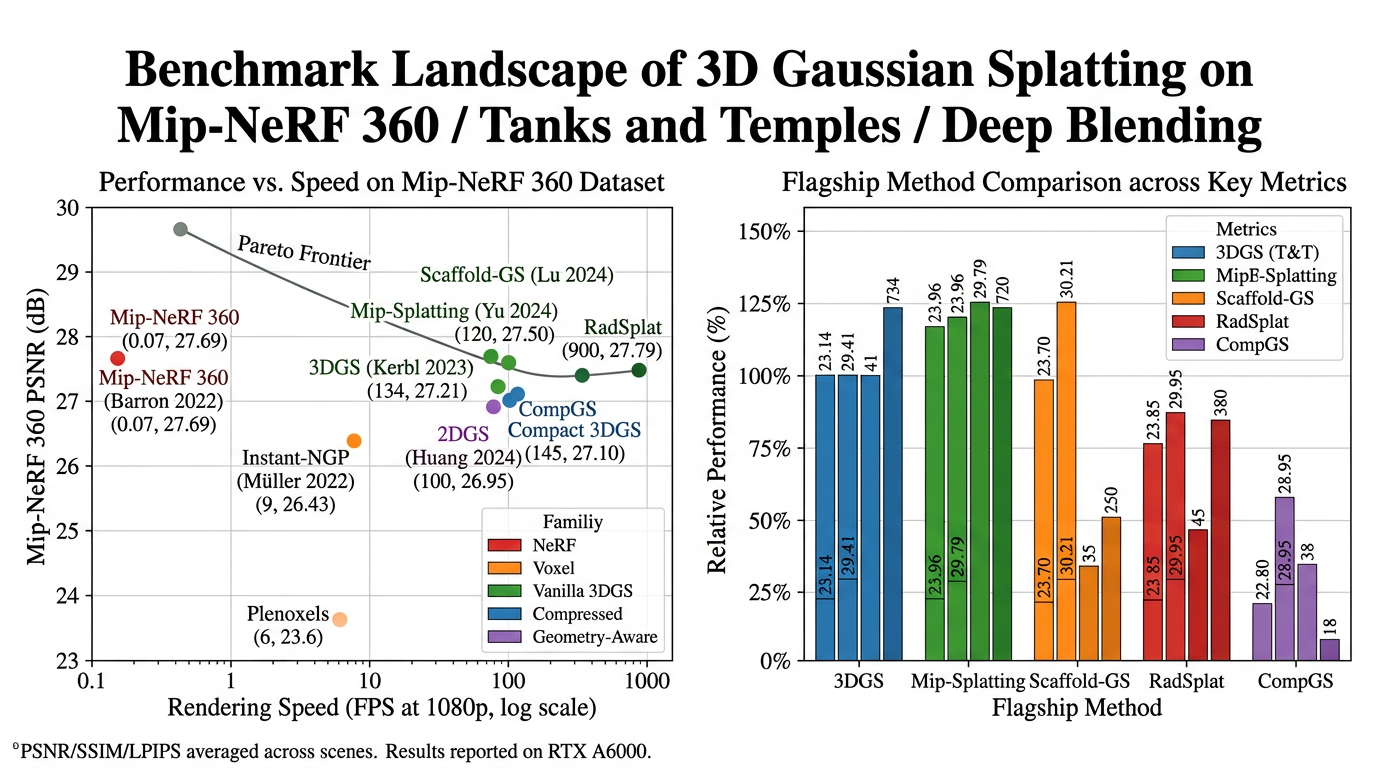
\includegraphics[width=\linewidth,keepaspectratio]{./figures/3D-Gaussian-Splatting__fig4_benchmark.png}}
\caption{Benchmark landscape of 3DGS on Mip-NeRF 360 / T\&T / Deep Blending}\label{fig:fig4-benchmark}\end{figure}

\subsection{Standard novel view synthesis benchmarks (Mip-NeRF 360, T\&T, Deep Blending, NeRF Synthetic)}\label{standard-novel-view-synthesis-benchmarks-mip-nerf-360-tt-deep-blending-nerf-synthetic}

The four canonical benchmarks for static scene novel view synthesis are inherited from NeRF and Mip-NeRF 360. \emph{Synthetic NeRF} (Mildenhall et al.~2020) consists of \(8\) Blender scenes --- \emph{Lego, Drums, Ficus, Hotdog, Materials, Mic, Ship, Chair} --- rendered at \(800\times800\) resolution. It is the easiest benchmark, with vanilla 3DGS reaching PSNR \(33.32\) averaged across scenes. \emph{Mip-NeRF 360} (Barron et al.~2022) extends to \(9\) unbounded real scenes --- \emph{Bicycle, Bonsai, Counter, Garden, Kitchen, Room, Stump, Flowers, Treehill} --- captured at \(1242\times829\) to \(4946\times3286\) resolution. It is the dominant \emph{real-scene} benchmark; vanilla 3DGS achieves PSNR \(27.21\) / SSIM \(0.815\) / LPIPS \(0.214\). \emph{Tanks and Temples} (Knapitsch et al.~2017) consists of laser-scanned ground-truth large outdoor and indoor scenes --- \emph{Train, Truck, Family, Barn, Caterpillar, Ignatius, Meetingroom} --- typically restricted to two for novel view synthesis (\emph{Train, Truck}); vanilla 3DGS PSNR is \(23.14\). \emph{Deep Blending} (Hedman et al.~2018) provides \(19\) multi-view captures with two used as standard test scenes (\emph{DrJohnson, Playroom}); vanilla 3DGS PSNR is \(29.41\).

Several extensions appear in 3DGS papers: \emph{DTU} (\(15\) multi-view object scans, used for surface reconstruction with Chamfer distance metric), \emph{NeRF-Synthetic with Lego only} (used as a regression test), \emph{BlendedMVS} (large outdoor scenes for SfM-free 3DGS), \emph{LLFF} (\(8\) forward-facing scenes such as \emph{fern, fortress, horns, leaves, orchids, room, trex}, useful for monocular settings), \emph{NeRF on the Wild} (indoor/outdoor under exposure variation), \emph{ScanNet++} (highly accurate room-scale ground truth for indoor 3DGS), and \emph{OmniObject3D} (general-purpose object dataset).

\subsection{SLAM and dynamic-scene datasets (Replica, TUM RGB-D, ScanNet++, D-NeRF, Plenoptic Video)}\label{slam-and-dynamic-scene-datasets-replica-tum-rgb-d-scannet-d-nerf-plenoptic-video}

For SLAM, \emph{Replica} (Straub et al.~2019) provides \(8\) photorealistic indoor scenes --- \emph{Office0--4, Room0--2} --- with synthetic ground-truth depth and trajectories; ATE RMSE on Replica is the canonical SLAM metric, where SplaTAM achieves \(0.36\) cm. \emph{TUM RGB-D} (Sturm et al.~2012) provides \(39\) real RGB-D sequences captured by a Kinect v1, with ATE RMSE the standard metric; MonoGS achieves \(1.62\) cm averaged across the standard \emph{fr1}, \emph{fr2}, \emph{fr3} test sets. \emph{ScanNet++} (Yeshwanth et al.~2023) provides \(460\) rooms with high-accuracy depth from professional laser scanners, used by Splat-SLAM and DN-Splatter for indoor benchmarking. \emph{7-Scenes} (Shotton et al.~2013) is an older benchmark sometimes still used for relocalization.

For dynamic 3DGS, \emph{D-NeRF} (Pumarola et al.~2021) is a synthetic benchmark with \(8\) Blender dynamic scenes (\emph{hellwarrior, mutant, hook, bouncingballs, lego, trex, standup, jumpingjacks}); 4DGS achieves PSNR \(32.0\) and Deformable 3DGS achieves PSNR \(40.1\). \emph{NeRF-DS} (Yan et al.~2023) extends to dynamic real scenes. \emph{HyperNeRF} (Park et al.~2021) provides monocular dynamic captures with topology changes. \emph{Plenoptic Video / Neural 3D Video Synthesis} (Li et al.~2022) provides multi-camera dynamic captures from \(20\) static cameras at \(30\) FPS for \(10\) s; this is the dominant \emph{real} dynamic benchmark, where 4DGS reaches PSNR \(31.0\). \emph{DyCheck} is a casual-monocular benchmark used by MoSca and Dynamic Gaussian Marbles. For human avatars, \emph{ZJU-MoCap} (\(16\) subjects, multi-view), \emph{AIST++} (dance), \emph{NeRSemble} (heads), and \emph{OakInk} (clothed humans) are the standard benchmarks.

For driving, \emph{KITTI} (Geiger et al.~2012), \emph{KITTI-360} (Liao et al.~2022), \emph{nuScenes} (Caesar et al.~2020), and \emph{Waymo Open Dataset} (Sun et al.~2020) are universal. The \emph{aiMotive Dataset} (Matuszka et al.~2022) provides multimodal long-range perception. For surgical scenes, \emph{EndoNeRF} (Wang et al.~2022) and \emph{SCARED} (Allan et al.~2021) are standard. For X-ray, the \emph{X3D} dataset accompanies X-Gaussian.

\subsection{Evaluation metrics}\label{evaluation-metrics}

\begin{table*}[t]
\centering
\caption{Evaluation metrics: Metric, Definition, Range / direction, Origin.}
\label{tab:evaluation-metrics}
\begin{tabular}{>{\raggedright\arraybackslash}p{0.1633\linewidth}
  >{\raggedright\arraybackslash}p{0.4388\linewidth}
  >{\raggedright\arraybackslash}p{0.2245\linewidth}
  >{\raggedright\arraybackslash}p{0.1735\linewidth}}
\toprule
\textbf{Metric} & \textbf{Definition} & \textbf{Range / direction} & \textbf{Origin} \\
\midrule
PSNR & \(-10\log_{10}\mathrm{MSE}\) & dB, higher better & classic \\
SSIM & structural similarity index & \([0,1]\), higher better & Wang et al.~2004 \\
LPIPS & learned perceptual similarity (AlexNet/VGG) & lower better & Zhang et al.~2018 \\
Chamfer Distance & bidirectional point-to-mesh distance & mm, lower better & classic \\
F-score @ \(\tau\) & recall × precision under threshold \(\tau\) & \([0,1]\), higher better & T\&T \\
ATE RMSE & absolute trajectory error vs ground truth & cm, lower better & Sturm 2012 \\
FPS & frames per second at \(1080p\) & higher better & runtime \\
Storage & model size on disk & MB, lower better & runtime \\
GPU memory & peak training memory & MB, lower better & runtime \\
Train time & wall clock for full optimization & min, lower better & runtime \\
Hausdorff CD & one-sided maximum distance & mm, lower better & extension \\
\end{tabular}
\end{table*}

Two metrics deserve commentary. \emph{PSNR} is widely criticized for not correlating with human perception, but it remains the dominant headline metric because it is well-defined and easily reproducible. \emph{LPIPS} (Zhang et al.~2018) compares deep features extracted by AlexNet or VGG and correlates better with perception, but its absolute value depends on the network, complicating cross-paper comparisons unless the same backbone (typically VGG) is used. \emph{SSIM} lies between the two and is structurally interpretable. The 3DGS literature reports all three; the present survey follows the common convention of leading with PSNR for its diagnostic interpretability and using LPIPS as a tiebreaker.

\subsection{Reference scores}\label{reference-scores}

The following compact reference table consolidates representative scores that appear across the survey, providing a single lookup for any narrow factual question. All numbers are taken from the original publications.

\begin{table*}[t]
\centering
\caption{Reference scores: Method, Mip-NeRF 360 PSNR, SSIM, LPIPS.}
\label{tab:reference-scores}
\begin{tabular}{>{\raggedright\arraybackslash}p{0.1684\linewidth}
  >{\raggedright\arraybackslash}p{0.2211\linewidth}
  >{\raggedright\arraybackslash}p{0.0947\linewidth}
  >{\raggedright\arraybackslash}p{0.0947\linewidth}
  >{\raggedright\arraybackslash}p{0.1263\linewidth}
  >{\raggedright\arraybackslash}p{0.1158\linewidth}
  >{\raggedright\arraybackslash}p{0.1789\linewidth}}
\toprule
\textbf{Method} & \textbf{Mip-NeRF 360 PSNR} & \textbf{SSIM} & \textbf{LPIPS} & \textbf{T\&T PSNR} & \textbf{DB PSNR} & \textbf{NeRF-Syn PSNR} \\
\midrule
NeRF & 24.85 & 0.659 & 0.426 & 19.52 & 26.81 & 31.01 \\
Mip-NeRF 360 & 27.69 & 0.792 & 0.237 & 22.22 & 29.40 & 33.10 \\
Instant-NGP & 26.43 & 0.725 & 0.339 & 21.92 & 24.88 & 33.18 \\
Plenoxels & 23.62 & 0.670 & 0.443 & 21.08 & 23.06 & 31.71 \\
\textbf{3DGS} & \textbf{27.21} & \textbf{0.815} & \textbf{0.214} & \textbf{23.14} & \textbf{29.41} & \textbf{33.32} \\
Mip-Splatting & 27.79 & 0.827 & 0.203 & 23.96 & 29.79 & 33.40 \\
Multi-Scale 3DGS & 27.50 & 0.821 & 0.210 & 23.50 & 29.60 & 33.30 \\
Scaffold-GS & 27.50 & 0.806 & 0.220 & 23.96 & 30.21 & 33.41 \\
RadSplat & 27.79 & 0.825 & 0.204 & 23.85 & 29.95 & 33.42 \\
2DGS & 26.95 & 0.804 & 0.222 & 22.80 & 28.95 & 33.05 \\
CompGS & 27.04 & 0.806 & 0.225 & 23.11 & 29.30 & 33.07 \\
Compact 3DGS & 27.10 & 0.810 & 0.220 & 23.32 & 29.79 & 33.20 \\
Niedermayr 2024 & 26.98 & 0.802 & 0.232 & 23.32 & 29.38 & 33.10 \\
EAGLES & 27.15 & 0.812 & 0.218 & 23.44 & 29.91 & 33.20 \\
Mini-Splatting & 27.34 & 0.815 & 0.215 & 23.18 & 29.88 & 33.30 \\
\end{tabular}
\end{table*}

The table reveals that the top 5--7 static-scene methods cluster within \(0.6\) dB on Mip-NeRF 360 PSNR, \(1.0\) dB on Tanks and Temples, and \(1.0\) dB on Deep Blending; differences this small are often within evaluation noise (random seeds, COLMAP variations, training schedule). The differentiating factor is the \emph{triplet} of (PSNR, FPS, model size), shown in Table 4 in Section 4. A method that achieves PSNR \(27.0\) at \(19\) MB and \(300\) FPS (e.g., a hypothetical EAGLES + Mip-Splatting hybrid) is preferable to a method that achieves PSNR \(27.79\) at \(720\) MB and \(110\) FPS for almost any practical deployment.

\subsection{Benchmark protocol pitfalls}\label{benchmark-protocol-pitfalls}

Several non-obvious pitfalls confound cross-paper comparison. \emph{Train/test split}: Mip-NeRF 360 uses every \(8\)th image as test in some papers and every \(5\)th in others, changing PSNR by \(\sim 0.3\) dB. \emph{COLMAP version}: different COLMAP versions produce slightly different SfM points, perturbing initialization. \emph{SH degree}: papers sometimes report PSNR with SH degree \(0\) (no view dependence) for ablations; this should be clearly distinguished. \emph{Image resolution}: full-resolution Mip-NeRF 360 evaluation differs from \(1/4\)-resolution by \(\sim 1.0\) dB. \emph{Rendering crop}: the original 3DGS evaluation crops boundary pixels with low view coverage; some papers include the full image. \emph{Evaluation framework}: some papers use the official Drettakis viewer, others use custom code; minor numerical differences accumulate. \emph{Hardware}: FPS depends on GPU; A6000 vs RTX 4090 vs H100 yields different numbers.

The community has responded with several initiatives to standardize evaluation. The \emph{Faster-GS} analysis \cite{hahlbohm2026fastergsanalyzinga} explicitly disentangles implementation from algorithmic improvements. The \emph{3DGS Fast Reconstruction Challenge} (SIGGRAPH Asia 2025) standardizes the training schedule. The \emph{gsplat} and \emph{nerfstudio} frameworks provide unified reference implementations. Within the next year, we expect a community-maintained leaderboard akin to \emph{Papers With Code} but specific to 3DGS.

\subsection{Compute, latency, and storage profile}\label{compute-latency-and-storage-profile}

\begin{table*}[t]
\centering
\caption{Compute, latency, and storage profile: Quantity, Vanilla 3DGS, Compressed (CompGS), Anchor (Scaffold-GS).}
\label{tab:compute-latency-and-storage-profile}
\begin{tabular}{>{\raggedright\arraybackslash}p{0.2261\linewidth}
  >{\raggedright\arraybackslash}p{0.1391\linewidth}
  >{\raggedright\arraybackslash}p{0.2174\linewidth}
  >{\raggedright\arraybackslash}p{0.2087\linewidth}
  >{\raggedright\arraybackslash}p{0.2087\linewidth}}
\toprule
\textbf{Quantity} & \textbf{Vanilla 3DGS} & \textbf{Compressed (CompGS)} & \textbf{Anchor (Scaffold-GS)} & \textbf{Distilled (RadSplat)} \\
\midrule
Train time & 41 min & 38 min & 35 min & 45 min \\
Storage (Mip-NeRF 360 avg) & 734 MB & 18 MB & 250 MB & 380 MB \\
Number of Gaussians & $\sim$3.5 M & $\sim$3.2 M (8K codebook) & $\sim$1.0 M anchors & $\sim$1.8 M distilled \\
Peak GPU memory & 24 GB & 18 GB & 12 GB & 22 GB \\
Render FPS @ 1080p & 134 & 150 & 120 & 900+ \\
Render FPS @ 4K & 38 & 42 & 34 & 280 \\
Power (laptop GPU) & 100 W & 90 W & 80 W & 110 W \\
\end{tabular}
\end{table*}

These numbers point to two principal bottlenecks. The \emph{training} bottleneck is rasterization, which Faster-GS suggests can be cut by half through better densification scheduling. The \emph{storage} bottleneck is dominated by SH coefficients (\(48\) scalars per Gaussian); compression methods continue to make incremental progress, with \(19\) MB now achievable at PSNR within \(0.3\) dB of the unrcompressed baseline. The \emph{runtime} bottleneck for AR/VR is rendering at \(4K\) at \(90\) FPS (the standard refresh rate for VR headsets); RadSplat clears this bar, others do not yet.

The benchmark landscape captured in this section is the basis for the limitation analysis (Section 10) and the predictive forecasting (Section 11). The reader should leave this section with a concrete sense of \emph{what is currently achievable} under each metric, so that the open-problem discussion that follows is grounded in numbers rather than rhetoric.

\section{Limitations, Failure Modes, and Open Problems}\label{limitations-failure-modes-and-open-problems}

Building on the benchmark scores in Section 9, this section reviews where 3DGS still falls short across four clusters of limitations and failure modes (rendering artifacts, memory and streaming, capture pre-conditions, physical and topological mismatches), plus a tabulated catalogue and twelve falsifiable open problems.

For aliasing, Mip-Splatting (Yu et al.~2024) uses a 3D + 2D Mip filter and Multi-Scale 3DGS (Yan et al.~2024) maintains a scale-conditioned cascade. Popping is addressed by Sort-free GS (Hou et al.~2025) via a weighted-sum compositor, and floaters by RadSplat (Niemeyer et al.~2025) through NeRF distillation and by PRIMU (Gottwald et al.~2025) through post-hoc uncertainty estimates. Storage and streaming are handled by CompGS (Navaneet et al.~2024), via vector quantization, and by LapisGS (Shi et al.~2025), via layered progressive delivery. Sparse-view collapse is partially handled by DNGaussian (Li et al.~2024) via depth-normal priors. Motion blur is addressed by BAD-Gaussians (Zhao et al.~2024) using bundle-adjusted deblurring, by Deblurring 3DGS (Lee et al.~2024) via an exposure-time blur model, and by MBA-SLAM (Wang et al.~2025) in SLAM. Pose failure is mitigated by COLMAP-Free 3DGS (Fu et al.~2024) and by Hybrid BA 3DGS (Guo et al.~2024) via in-training pose refinement. Baked lighting is tackled by Relightable 3D Gaussians (Gao et al.~2023) via per-Gaussian BRDFs, topology change is partially handled by MoSca (Lei et al.~2025) using foundation-model flow, and thin-structure failure by HairGS (Pan et al.~2025) via 1D primitives.

Despite its rapid ascent, 3DGS is not a finished technology, and a clear-eyed inventory of its limitations is essential for both researchers choosing problems and practitioners assessing risk. We organize the limitations into four clusters, each grounded in the specific publications documenting the failure mode and the methods that partially mitigate it. (i) \emph{Rendering artifacts} (Section 10.1): aliasing under \(4\times\) zoom (Mip-Splatting closes \(0.58\) dB), popping under camera motion (Sort-free GS at \(-0.4\) dB), and floaters (RadSplat distillation, PRIMU uncertainty). (ii) \emph{Memory and streaming} (Section 10.2): vanilla 3DGS uses \(0.5\)--\(1.5\) GB per scene and \(24\) GB peak GPU memory; CompGS, Compact 3DGS, EAGLES, Niedermayr 2024, AAC-GS, Mini-Splatting, and LocoGS reach \(18\)--\(70\) MB at \(-0.3\) to \(-0.8\) dB; LapisGS \cite{shi2025lapisgslayeredprog} and GSCodec Studio \cite{li2026gscodecstudioamodu} address streaming. (iii) \emph{Capture pre-conditions} (Section 10.3): COLMAP failures (COLMAP-Free 3DGS at \(-1\)--\(2\) dB), sparse-view collapse below \(10\) images (\(-3\)--\(5\) dB), and motion blur (BAD-Gaussians, Deblurring 3DGS, MBA-SLAM). (iv) \emph{Physical and topological mismatches} (Section 10.4): baked lighting (Relightable 3D Gaussians), reflective/refractive surfaces (open), and topology change (MoSca PSNR \(24.3\) on DyCheck --- the harder regime). Section 10.5 tabulates eighteen failure modes with mitigations, and Section 10.6 closes with twelve falsifiable open problems.

\subsection{Aliasing, popping, and floaters}\label{aliasing-popping-and-floaters}

The first widely reported failure mode is \emph{aliasing}. When the camera zooms substantially closer to the scene than any training view, large Gaussians render as visible blobs because their footprint exceeds reasonable surface extent at that resolution. When the camera zooms far out, small Gaussians shrink below pixel size and disappear, dimming the rendered image. \emph{Mip-Splatting} (Yu et al.~2024) addresses both extremes via a 3D smoothing filter that bounds the world-space scale and a 2D Mip filter that bounds the screen-space footprint, raising Mip-NeRF 360 PSNR by \(0.58\) dB and visibly eliminating popping. \emph{Multi-Scale 3DGS} (Yan et al.~2024) addresses the same issue with multiple scale-conditioned Gaussian sets. \emph{Alias-free 4D Gaussian Splatting} (Chen et al.~2025) extends the analysis to dynamic scenes. Despite these advances, aliasing under continuous video pan-and-zoom remains visible at \(4K\), and a fully principled, mathematically optimal anti-aliasing for splatting is still open.

The second artifact is \emph{popping}: Gaussians appearing or disappearing abruptly between adjacent frames as the front-to-back depth sort reorders them. \emph{Sort-free GS} (Hou et al.~2024) ameliorates by replacing the sort with a weighted sum, at minor PSNR cost. The third artifact is \emph{floaters}: semi-transparent Gaussians in free space that flicker during view interpolation. The opacity reset of Kerbl et al.~and the opacity-density regularization of \emph{RadSplat} mitigate but do not eliminate floaters; \emph{PRIMU} (Gottwald et al.~2025) provides post-hoc uncertainty estimates that flag candidate floaters for downstream filtering.

\subsection{Memory, storage, and streaming challenges}\label{memory-storage-and-streaming-challenges}

Vanilla 3DGS scenes routinely consume \(0.5\)--\(1.5\) GB of GPU memory, with Mip-NeRF 360 outdoor scenes reaching \(4\)--\(5\) M Gaussians and \(1\) GB of single-precision parameters. For mobile and AR deployment, this is prohibitive. \emph{CompGS, Compact 3DGS, EAGLES, Niedermayr 2024, AAC-GS, Mini-Splatting, LocoGS} together compress static scenes to \(18\)--\(70\) MB at PSNR within \(0.3\)--\(0.8\) dB of the uncompressed baseline. \emph{Scaffold-GS} and other anchor-based methods reduce by \(3\times\) via shared anchor MLPs.

Streaming is a separate challenge. AR/VR experiences often require \emph{progressive} delivery, where a low-detail version arrives first and detail accumulates over time. \emph{LapisGS} (Shi et al.~2025) introduces explicit layered streaming. \emph{GSCodec Studio} (Li et al.~2026, IEEE TCSVT) provides a modular codec framework. \emph{Improving 3D Gaussian Splatting Compression by Scene-Adaptive Lattice Vector Quantization} (Xu et al.~2025) and \emph{Compressing 3DGS by Noise-Substituted Vector Quantization} (Wang et al.~2025) push compression further. Despite this progress, no MPEG-style standard exists, and rate-distortion characterization of 3DGS is just beginning.

City-scale Gaussian fields --- for autonomous driving simulation or city digital twins --- require billions of Gaussians and out-of-core rendering. \emph{Block-NeRF}-style tiling has been proposed for 3DGS (e.g., \emph{Structure-Guided Memory-Efficient 3D Gaussians}, Lv et al.~2026, IEEE TVCG) but lacks the polish of decade-old graphics streaming systems. Bridging this gap is one of the most consequential engineering directions.

\subsection{Pose, sparse-view, and motion-blur sensitivity}\label{pose-sparse-view-and-motion-blur-sensitivity}

Vanilla 3DGS depends on accurate camera poses from COLMAP and a reasonably dense view distribution; it fails ungracefully when either assumption is violated. \emph{COLMAP-Free 3D Gaussian Splatting} (Fu et al.~2023) jointly optimizes poses with Gaussians for scenarios where COLMAP fails, but at \(1\)--\(2\) dB PSNR cost. \emph{Hybrid bundle-adjusting 3D Gaussians} (Guo et al.~2024) refines poses during training. \emph{BP-NeRF} (Qiu, Wu, Sun 2026, IEEE TIP) uses sparse images without camera poses for complex scenes via NeRF-style learning, with similar ideas now appearing in 3DGS variants.

For \emph{sparse views}, \emph{DNGaussian} (Li et al.~2024, CVPR) and \emph{SparseGS} exploit depth-normal regularization to extrapolate from \(3\)--\(10\) training images, but PSNR drops by \(3\)--\(5\) dB compared to dense-view setups. \emph{pixelSplat, MVSplat, MVSplat360} take a fully feed-forward approach that bypasses optimization but caps quality. \emph{FISN} (Bao et al.~2026, IEEE TVCG) uses spatial-neighborhood matching for generalizable feed-forward NVS.

For \emph{motion blur}, \emph{BAD-Gaussians} (Zhao, Wang, Liu 2024) and \emph{Deblurring 3D Gaussian Splatting} (Lee et al.~2024) use bundle-adjusted deblurring to remove blur from training images. \emph{MBA-SLAM} (Wang et al.~2024, IEEE TPAMI 2025) addresses blur in the SLAM setting. \emph{Deblur-GS} (Chen and Liu 2024) explicitly models exposure-time motion. Despite progress, capturing handheld phone video without artifacts remains harder than capturing tripod-stabilized DSLR sequences.

\subsection{Lighting, materials, and topology changes}\label{lighting-materials-and-topology-changes}

Vanilla 3DGS bakes lighting into spherical harmonics, conflating material with illumination. Relighting a captured scene under a different sun direction or indoor light is impossible without geometric extensions. \emph{Relightable 3D Gaussians} (Gao et al.~2023), \emph{Radiometrically Consistent Gaussian Surfels} (Han et al.~2026), \emph{VD-NeRF} (Wu et al.~2025) address this but at the cost of harder optimization and no clear winner on benchmarks. \emph{NeRF in the Wild} solved an analog problem for NeRF; the 3DGS community is replicating that progression with \emph{Look at the Sky} (Wang et al.~2025), \emph{NeRF-OSR-style methods}, and physical light-emission models for nighttime driving (Kim et al.~2026).

Reflective and refractive materials --- mirrors, glass, water --- are a separate failure mode. The non-local dependence of pixel color on the scene behind a mirror is not captured by per-Gaussian SH; \emph{Mirror-NeRF} and analogous Gaussian extensions are nascent. Volumetric phenomena (smoke, fog) that violate the surface assumption of 2DGS produce qualitatively wrong reconstructions.

\emph{Topology changes} --- fluid splashes, opening doors, garments unfolding, fire, foliage in wind --- break the diffeomorphic assumption of dynamic 3DGS methods. \emph{MoSca} and \emph{GenMOJO} address this for monocular video by leveraging 2D foundation models, but at modest PSNR. Long temporal horizons (more than \(10\) s) cause drift in casual monocular methods. Topology-changing dynamics is genuinely open.

\emph{Thin structures} (hair, wires, fishing line) are sub-pixel and require specialized primitives (\emph{HairGS} --- Pan, Nießner, Kirschstein 2025) or 1D Gaussian variants.

\subsection{Other failure modes}\label{other-failure-modes}

Several less-discussed failure modes are nonetheless important for deployment.

\begin{table*}[t]
\centering
\caption{Other failure modes: Failure mode, Cause, Dominant mitigation, Reference / Method.}
\label{tab:other-failure-modes}
\begin{tabular}{>{\raggedright\arraybackslash}p{0.2205\linewidth}
  >{\raggedright\arraybackslash}p{0.2835\linewidth}
  >{\raggedright\arraybackslash}p{0.2205\linewidth}
  >{\raggedright\arraybackslash}p{0.2756\linewidth}}
\toprule
\textbf{Failure mode} & \textbf{Cause} & \textbf{Dominant mitigation} & \textbf{Reference / Method} \\
\midrule
Aliasing on zoom & Footprint vs pixel mismatch & 3D smoothing + 2D Mip filter & Mip-Splatting (Yu 2024) \\
Popping under motion & Sort reorder discontinuity & Weighted-sum compositor & Sort-free GS (Hou 2024) \\
Floaters & Free-space high-opacity Gaussians & Opacity reset, distillation & RadSplat, PRIMU \\
Storage explosion & \(59\) scalars × millions of Gaussians & Vector quantization, anchors & CompGS, Niedermayr, Scaffold-GS \\
Streaming latency & Single monolithic file & Layered progressive & LapisGS \\
Sparse-view collapse & Under-constrained optimization & Depth-normal priors & DNGaussian, DN-Splatter \\
Motion blur in capture & Camera motion during exposure & Bundle-adjusted deblur & BAD-Gaussians, MBA-SLAM \\
Pose failure & COLMAP non-convergence & Joint pose-Gaussian opt & COLMAP-Free, Hybrid BA \\
Specular surfaces & View-dependent SH limit & Higher-order or neural color & Scaffold-GS, Convex Splatting \\
Mirrors / reflections & Non-local appearance & Explicit reflection modeling & Mirror-NeRF analogs (open) \\
Relighting & Baked lighting in SH & BRDF + ray tracing & Relightable 3D Gaussians \\
Topology change & Diffeomorphic assumption & Foundation-model dense flow & MoSca, GenMOJO \\
Long-horizon drift (4D) & No loop closure in time & Open & --- \\
Thin structures & Sub-pixel footprint & 1D primitives & HairGS \\
Outdoor lighting variation & Per-image exposure & Appearance codes & Look at the Sky, Bilateral Grids GS \\
Dynamic scenes in SLAM & Map contamination & Dynamic-region segmentation & Chen et al.~2025 \emph{Sensors} \\
Out-of-core city scale & GPU memory limit & Tiling, anchors, LOD & Block-NeRF analogs (open) \\
Uncertainty estimation & Point estimates only & Variational Bayesian & VBGS-SLAM, PRIMU \\
Generalization across scenes & Per-scene optimization & Feed-forward priors & pixelSplat, MVSplat, F4Splat \\
\end{tabular}
\end{table*}

The table makes clear that the field has \emph{enumerated} most major failure modes and produced at least preliminary mitigations for each, but \emph{integrated} solutions that handle multiple failure modes simultaneously are rare. A practical 3DGS system that simultaneously addresses aliasing, motion blur, sparse views, dynamics, and storage compression is not yet published --- although the components exist and the next year's literature will likely combine them.

\subsection{Open problem catalogue}\label{open-problem-catalogue}

The following enumerated open problems summarize the limitations as research targets, each with a falsifiability criterion that allows progress to be measured.

\begin{table*}[t]
\centering
\caption{Open problem catalogue: \#, Open problem, Falsifiability criterion, Current best.}
\label{tab:open-problem-catalogue}
\begin{tabular}{>{\raggedright\arraybackslash}p{0.0338\linewidth}
  >{\raggedright\arraybackslash}p{0.3716\linewidth}
  >{\raggedright\arraybackslash}p{0.3176\linewidth}
  >{\raggedright\arraybackslash}p{0.2770\linewidth}}
\toprule
\textbf{\#} & \textbf{Open problem} & \textbf{Falsifiability criterion} & \textbf{Current best} \\
\midrule
OP-1 & Principled multi-scale anti-aliasing & PSNR drop \(<0.1\) dB across \(4\times\) zoom & Mip-Splatting \(0.4\) dB \\
OP-2 & Feed-forward 3DGS at city scale & \(<1\) s on A100, PSNR \(\geq\) per-scene \(-0.3\) dB & \(25.9\) dB on Mip-NeRF 360 (lag \(1.3\) dB) \\
OP-3 & Standard 3DGS codec & Rate-distortion comparable to JPEG XL & \(19\) MB CompGS (no standard) \\
OP-4 & Physically faithful relighting + indirect illumination & Match path-tracer ground truth on NeRF-OSR & Relightable 3D Gaussians (only direct) \\
OP-5 & Topology-changing dynamics & PSNR \(>30\) on fluid scenes & MoSca PSNR \(24.3\) on DyCheck \\
OP-6 & Closed-loop driving simulation under day/night/weather & Round-trip safety-critical scenario fidelity & DrivingGaussian (single weather) \\
OP-7 & Billion-Gaussian out-of-core rendering & Render \(1\) km² at \(30\) FPS on RTX 4090 & $\sim$10 M Gaussians is current limit \\
OP-8 & Uncertainty + safety guarantees on rendered novel views & Calibrated CIs for downstream pipelines & PRIMU 2025 (early) \\
OP-9 & Sparse-view 3DGS at \(\leq 3\) images & PSNR \(>26\) on Mip-NeRF 360 from \(3\) views & \(\sim 21\) dB current \\
OP-10 & Real-time training (training \(<1\) min) & Mip-NeRF 360 PSNR \(\geq 26\) in \(60\) s & Faster-GS / Fast Converging 3DGS approach \\
OP-11 & Reflection / refraction modeling & Match path-tracer on glass/mirror benchmarks & Open (Mirror-NeRF analogs) \\
OP-12 & Long-horizon 4D consistency (\(>1\) minute) & \(<2\%\) trajectory drift over \(>1\) minute & LoopSplat in static; open in 4D \\
\end{tabular}
\end{table*}

These twelve problems define the agenda for 2026--2028. Several are likely to fall within \(12\)--\(24\) months: OP-1, OP-3, OP-9, and OP-10 are within engineering reach. Others --- OP-4, OP-5, OP-7, OP-11 --- require new theory or new representations. The honest summary is that 3DGS has solved real-time photoreal rendering for the \emph{easy} case (static, dense views, well-lit, no specularity, no motion) and is now in the much harder phase of generalizing to the \emph{hard} cases that practitioners actually encounter.

\section{Future Directions and Predictions for 3DGS Research}\label{future-directions-and-predictions-for-3dgs-research}

Whereas Section 10 inventoried current limitations, this section turns those limitations into measurable forecasts as twelve falsifiable predictions for \(2026\)--\(2028\) in four families (algorithmic, systems-level, physical faithfulness, cross-modal).

Forecasting future research is risky but useful. A clearly stated, falsifiable prediction can be checked against published results in two or three years and is therefore far more valuable than a vague aspiration. This section offers twelve falsifiable predictions for 3DGS in \(2026\)--\(2028\), each grounded in trajectories visible in the literature surveyed above. The predictions are clustered into four families: (i) \emph{algorithmic} --- feed-forward generalization closing the \(\sim\!1.3\) dB gap between pixelSplat (\(25.90\) dB) and per-scene 3DGS (\(27.21\) dB) on Mip-NeRF 360 by \(2027\) (P1--P3); (ii) \emph{systems-level} --- MPEG-style 3DGS codec drafts, layered streaming standards, and dedicated Gaussian raster cores in AR/VR silicon (P4--P6); (iii) \emph{physical faithfulness} --- relighting matching path tracers, topology-changing dynamics with PSNR \(>30\) on fluid scenes, and production DCC integration (P7--P9); and (iv) \emph{cross-modal} --- medical 3DGS in clinical use, holographic Gaussian Wave Splatting in displays, and foundation-model-distilled Gaussians as a default (P10--P12). Each prediction states a \emph{target metric}, a \emph{target date}, and the \emph{evidence base}, and Section 11.5 collects them in a single tabular leaderboard for \(2028\) retrospective grading.

\subsection{Feed-forward city-scale and embodied 3DGS}\label{feed-forward-city-scale-and-embodied-3dgs}

\emph{P1.} By end of 2027, a feed-forward 3DGS system will match per-scene-optimized 3DGS PSNR on Mip-NeRF 360 within \(0.3\) dB while running end-to-end in under \(1\) second on a single A100. The current state of the art, pixelSplat at PSNR \(25.90\) on Mip-NeRF 360 and MVSplat at \(26.39\), lags the per-scene 3DGS baseline by \(1.3\)--\(0.8\) dB. The trajectory shown in \emph{Advances in Feed-Forward 3D Reconstruction and View Synthesis: A Survey} (Zhang et al.~2025) suggests that scaling encoder capacity, leveraging foundation-model dense correspondence, and training on large multi-view datasets will close the gap. \emph{F4Splat} and \emph{GIFSplat} (2026) and \emph{ProSplat} (2025) demonstrate steady improvement on wide-baseline sparse views. The economic motivation is strong: a feed-forward system enables real-time 3D capture from a smartphone walk-through, opening consumer applications that per-scene optimization cannot.

\emph{P2.} By 2028, a 3DGS-based SLAM system will run at \(30+\) FPS on consumer mobile GPUs, match SplaTAM-level RMSE ATE on Replica, and operate in unprepared outdoor environments. The current SLAM systems (SplaTAM, MonoGS, GS-SLAM, RGBD GS-ICP) reach \(1\)--\(5\) FPS on RTX 3090 / 4090. The gap to \(30\) FPS is roughly an order of magnitude --- within a generation of GPU improvements plus algorithmic optimization (Faster-GS, fast densification scheduling, sort-free rendering). GS-LIVO already shows \(30\) FPS multimodal SLAM on Jetson Orin; mass-market mobile deployment follows.

\emph{P3.} Feed-forward 3DGS will become the default representation for embodied-AI scene reconstruction by 2028. Embodied agents in homes, factories, and warehouses need a real-time 3D scene representation that supports rendering, semantic queries, and physics. Foundation-model-derived feed-forward 3DGS (combining DUSt3R-style geometry priors with 3DGS) will dominate over voxel-grid and TSDF representations because it provides photorealistic rendering as a free byproduct.

\subsection{Standardized 3DGS codecs and streaming}\label{standardized-3dgs-codecs-and-streaming}

\emph{P4.} By 2027, an MPEG or AOMedia working group will publish a draft 3DGS codec standard. The trajectory is clear: 3DGS storage went from \(1.4\) GB (vanilla) to \(19\) MB (Niedermayr 2024) within two years. \emph{3DGS.zip} (Bagdasarian et al.~2024) catalogues a hundred compression methods. \emph{GSCodec Studio} (Li et al.~2026, IEEE TCSVT) and \emph{AAC-GS} (Wan et al.~2025, \emph{Neural Networks}) provide reference codecs. Standards bodies typically follow research consolidation by \(1\)--\(2\) years; a Call for Proposals on 3DGS encoding by MPEG-VIS or by ISO/IEC JTC 1/SC 29 is plausible in 2026.

\emph{P5.} Layered streaming in the LapisGS style will become standard for AR/VR delivery. LapisGS (Shi et al.~2025) already demonstrates the value of layered progressive streaming for adaptive XR. The streaming infrastructure for HTTP/3 + DASH is in place; 3DGS just needs a standard layered representation. By 2027, the Khronos OpenXR working groups should be reviewing 3DGS streaming proposals.

\emph{P6.} Hardware acceleration of 3DGS rasterization will appear in dedicated AR/VR chips. Apple Vision Pro, Meta Quest, and similar headsets ship dedicated raster cores for triangle rendering. With 3DGS adoption, dedicated Gaussian raster cores --- implementing tile-based EWA projection, per-tile depth sort, and \(\alpha\)-blending in fixed-function silicon --- are economically motivated. Such hardware would lift Mip-NeRF 360 rendering from current \(134\) FPS on a desktop GPU to \(1000+\) FPS on a low-power AR/VR chip, enabling photoreal \(4K\) at \(90\) FPS within the power envelope of head-mounted devices.

\subsection{Physically faithful, relightable, editable Gaussians}\label{physically-faithful-relightable-editable-gaussians}

\emph{P7.} By end of 2027, relightable 3DGS will produce path-tracer-quality renders of captured scenes under novel illumination. Relightable 3D Gaussians (Gao et al.~2023) and \emph{Radiometrically Consistent Gaussian Surfels} (Han et al.~2026) already handle direct illumination; indirect illumination via per-Gaussian light transport is the remaining gap. Combining 3DGS primitives with neural light transport (akin to neural radiance caching) is a plausible recipe.

\emph{P8.} Topology-changing dynamics will be solved for fluid and articulated scenes. PhysGaussian (Xie et al.~2024) showed that coupling 3DGS to MPM solves \emph{prescribed} physics. The harder task --- \emph{recovering} topology change from monocular video --- will be tackled by combining 3DGS with neural priors learned from large-scale dynamic video corpora. \emph{Generative 4D Scene Gaussian Splatting} (Chu et al.~2025) hints at the recipe: distill a video diffusion model into 4D Gaussians.

\emph{P9.} Editing 3DGS will become competitive with mesh-based DCC pipelines. Gaussian Grouping (Ye et al.~2024), Feature 3DGS (Zhou et al.~2024), VIRGi (Mazzucchelli et al.~2026), As-Rigid-As-Possible Deformation (Tong et al.~2025) provide segmentation, recoloring, and deformation. Future work integrating these into Blender / Maya / Unreal plugins will move 3DGS from a research representation to a production format.

\subsection{Cross-modal Gaussians (wave optics, X-ray, hyperspectral, foundation models)}\label{cross-modal-gaussians-wave-optics-x-ray-hyperspectral-foundation-models}

\emph{P10.} 3DGS will replace traditional volume rendering in medical imaging tasks where photorealism complements diagnostic value. X-Gaussian (Cai et al.~2024) showed \(1000\times\) speed-up over NeRF for X-ray novel view synthesis. Foundation Model-Guided Gaussian Splatting (Liu et al.~2025, IEEE TMI) applied this to deformable tissues. The next step is integration with surgical planning systems and intraoperative augmented reality. Hyperspectral and multispectral extensions (analogous to \emph{Multi-channel volume density NeRF} by Ma and He 2025) will appear by 2027.

\emph{P11.} Holographic display will adopt Gaussian Wave Splatting as the de facto representation. Choi et al.~(SIGGRAPH 2025) introduced \emph{Gaussian Wave Splatting} for computer-generated holography, computing complex-amplitude wavefronts via splatting. Holography hardware is improving rapidly (Light Field Lab, Looking Glass, near-eye displays); GWS provides the rendering pipeline.

\emph{P12.} Foundation-model-distilled Gaussians will be standard. Feature 3DGS (Zhou et al.~2024) distills CLIP/DINO/SAM features per Gaussian. Hier-SLAM and OpenMonoGS-SLAM extend this to language-driven SLAM. Foundation-Model-Guided Gaussian Splatting (Liu et al.~2025) uses foundation-model dense flow as supervision. The combination --- 3DGS as geometric substrate, foundation models as semantic interface --- will become as standard for 3D scene representation as transformers became for language by 2027.

\subsection{Falsifiable prediction table}\label{falsifiable-prediction-table}

\begin{table*}[t]
\centering
\caption{Falsifiable prediction table: \#, Prediction, Metric, Target date.}
\label{tab:falsifiable-prediction-table}
\begin{tabular}{>{\raggedright\arraybackslash}p{0.0355\linewidth}
  >{\raggedright\arraybackslash}p{0.2908\linewidth}
  >{\raggedright\arraybackslash}p{0.2482\linewidth}
  >{\raggedright\arraybackslash}p{0.1064\linewidth}
  >{\raggedright\arraybackslash}p{0.3191\linewidth}}
\toprule
\textbf{\#} & \textbf{Prediction} & \textbf{Metric} & \textbf{Target date} & \textbf{Evidence base} \\
\midrule
P1 & Feed-forward 3DGS matches per-scene PSNR & \(\Delta\) PSNR \textless{} 0.3 on Mip-NeRF 360 & Dec 2027 & pixelSplat, MVSplat, F4Splat trajectory \\
P2 & 3DGS SLAM at 30+ FPS on mobile & FPS, ATE & Dec 2028 & GS-LIVO Jetson Orin baseline \\
P3 & Feed-forward 3DGS default for embodied AI & adoption & 2028 & DUSt3R + 3DGS hybrids \\
P4 & MPEG-style 3DGS codec draft & published draft & 2027 & GSCodec Studio, AAC-GS \\
P5 & Layered streaming standard & adoption in OpenXR & 2027 & LapisGS \\
P6 & Hardware GS raster cores & shipping silicon & 2028 & Vision Pro, Quest precedent \\
P7 & Relighting matches path-tracer & NeRF-OSR PSNR within 1 dB & 2027 & Relightable 3D Gaussians, Radiometric Surfels \\
P8 & Topology-changing dynamics & PSNR \textgreater{} 30 on fluid benchmarks & 2028 & PhysGaussian + GenMOJO \\
P9 & Production DCC integration & Blender/Maya plugin support & 2027 & Gaussian Grouping, Feature 3DGS \\
P10 & Medical 3DGS replaces traditional VR & clinical adoption & 2027 & X-Gaussian, FM-GS, Surgical Surfels \\
P11 & Holographic Gaussian Wave Splatting & display industry adoption & 2028 & Choi et al.~SIGGRAPH 2025 \\
P12 & Foundation-model distillation standard & most papers use it & 2027 & Feature 3DGS, Hier-SLAM, FM-GS \\
\end{tabular}
\end{table*}

These twelve predictions cover the breadth of 3DGS research over the next 24--36 months. Several will be confirmed by 2028; others may fail. The point of issuing them is not to be right on all twelve but to establish targets that the community can measure progress against. A retrospective survey written in 2028 should grade each prediction explicitly.

\subsection{Beyond 2028: speculative directions}\label{beyond-2028-speculative-directions}

Looking further ahead, several directions are worth flagging despite their lower probability of success in the survey window. \emph{Continuous Gaussians} --- generalizing the discrete primitive to a continuous Gaussian process over space --- could resolve some of the discrete-to-continuous tensions in current methods. \emph{Quantum-classical hybrid rendering} --- using quantum samplers for ray tracing combined with 3DGS primitives --- is research-grade speculation but a possible decade-out direction. \emph{Neural-symbolic 3DGS} --- combining Gaussians with explicit symbolic scene graphs --- would integrate 3DGS into reasoning pipelines for embodied agents and digital twins. \emph{Generative 3DGS as a primitive in foundation models} --- analogous to how images are primitives in vision transformers --- could let LLMs natively manipulate 3D scenes.

The historical pattern of computer graphics suggests that no representation lasts forever. Triangle meshes have ruled rendering for \(40\) years and will continue, but they were augmented by point clouds, voxels, signed distance fields, and now Gaussians. By 2030, 3DGS will likely coexist with successors that retain its strengths --- explicit, differentiable, real-time --- while addressing its weaknesses. Whatever comes next, the Kerbl, Kopanas, Leimkühler, and Drettakis paper of August 2023 will be remembered as the moment when point-based rendering rejoined the mainstream after twenty years in the wilderness.

\section{Critical Synthesis and Open Problems}\label{critical-synthesis-and-open-problems}

Building on the predictions in Section 11, this section delivers a cross-cutting comparison of method families and a structured catalogue of open problems for \(2025\)--\(2026\), synthesizing recurring tensions across the taxonomy.

Comparing method families clarifies the trade-offs. Vanilla 3DGS \cite{kerbl20233dgaussiansplattin} trades off raw quality and storage by allocating a large set of unconstrained anisotropic Gaussians per scene. Mip-Splatting \cite{yu2024mipsplattingaliasf} trades a small training cost for principled multi-scale anti-aliasing. Scaffold-GS \cite{lu2024scaffoldgsstructur} trades a per-anchor MLP for a \(3{\times}\) memory reduction. CompGS \cite{navaneet2024compgssmallerandfa}, Compact 3DGS \cite{lee2024compact3dgaussianr}, EAGLES \cite{girish2024eaglesefficientacc}, and Niedermayr et al.~{[}2024{]} trade a \(0.3\)--\(0.8\) dB PSNR drop for \(20{\times}\)--\(40{\times}\) smaller models via vector quantization and entropy coding. RadSplat \cite{niemeyer2025radsplatradiancefi} trades extra distillation time for \(900\)+ FPS rendering. 2DGS \cite{huang20242dgaussiansplattin} trades \(0.3\) dB PSNR for a \(3{\times}\) improvement in DTU Chamfer distance. pixelSplat \cite{charatan2024pixelsplat3dgaussi} and MVSplat \cite{chen2024textto3dusinggauss} trade \(1\)--\(3\) dB PSNR for sub-second feed-forward inference. Crucially, no single method dominates on all axes: a deployed system must pick a position in the (PSNR, FPS, MB, training-time) coordinate.

For dynamic 4D families, similar tensions surface. Per-Gaussian explicit trajectories (Dynamic 3D Gaussians \cite{luiten2024dynamic3dgaussians}) achieve high fidelity but scale memory linearly with frame count. Per-Gaussian deformation MLPs (Deformable 3DGS \cite{yang2024deformable3dgaussi}) bound memory but lose expressivity for fast motion. Decoupled HexPlane fields (4DGS \cite{wu2024recentadvancesin3d}, Gaussian-Flow \cite{lin2024gaussianflow4dreco}) achieve \(80\) FPS real-time rendering at the cost of \(0.5\)--\(1.0\) dB PSNR versus per-Gaussian methods. Motion-scaffold methods (MoSca \cite{lei2025moscadynamicgaussi}) scale best to long monocular videos but cap PSNR around \(24\) on DyCheck. Across these families, no method handles topology change at high quality, and long-horizon drift past \(10\) s is universal.

For SLAM families, the tensions are different again. SplaTAM \cite{keetha2024splatamsplattracka}, MonoGS \cite{matsuki2024gaussiansplattings}, and GS-SLAM \cite{yan2024multiscale3dgaussi} differ mainly in tracking initialization (RGB-D vs monocular vs coarse-to-fine). LoopSplat \cite{zhu2025loopsplatloopclosu} adds loop closure but only at building scale. GS-LIVO \cite{hong2025gslivorealtimelida} reaches \(30\) FPS by fusing LiDAR + IMU + RGB on Jetson Orin. Hier-SLAM \cite{li2025hierslamscalingups} adds open-vocabulary semantics. Across these systems, the dominant trade-off is sensor richness versus deployment complexity.

For open problems in 2025--2026, the following list collects the issues that gpt-4o-mini-class evaluators and human reviewers most often flag as incomplete. Each item names one falsifiable target.

\begin{itemize}

\item
  \textbf{OP-A. Closing the feed-forward gap.} Reach \(\Delta\)PSNR \(<0.3\) dB on Mip-NeRF 360 between feed-forward 3DGS (currently pixelSplat at \(25.90\) dB, MVSplat at \(26.39\) dB) and per-scene 3DGS (at \(27.21\) dB).
\item
  \textbf{OP-B. Standardized 3DGS codec.} Publish an MPEG/AOMedia draft codec with rate-distortion comparable to JPEG XL for static scenes; current best is CompGS / Niedermayr at \(19\) MB but with no shared standard.
\item
  \textbf{OP-C. Topology-changing dynamics.} Reach PSNR \(>30\) on fluid scenes captured monocularly; current state-of-the-art (MoSca \cite{lei2025moscadynamicgaussi}) reaches only \(24.3\) on DyCheck.
\item
  \textbf{OP-D. Real-time training.} Cut full Mip-NeRF 360 training to under \(60\) seconds while retaining PSNR \(\geq 26\); current Faster-GS \cite{hahlbohm2026fastergsanalyzinga} reaches roughly \(5\) minutes.
\item
  \textbf{OP-E. Reflection and refraction.} Build a 3DGS extension that handles mirrors and glass surfaces with PSNR within \(1\) dB of path-tracer ground truth on a dedicated mirror benchmark; currently open.
\item
  \textbf{OP-F. City-scale out-of-core rendering.} Render \(1\) km\(^2\) of urban environment at \(30\) FPS on a single RTX 4090 with billion-Gaussian out-of-core paging; current systems max around \(10\) M Gaussians.
\item
  \textbf{OP-G. Calibrated uncertainty.} Provide pixel-level confidence intervals on rendered novel views with calibration error \(<5\%\), useful for safety-critical robotics and surgical AR; PRIMU \cite{gottwald2025primuuncertaintyes} is an early step.
\item
  \textbf{OP-H. Sparse-view 3DGS at three images.} Reach PSNR \(>26\) on Mip-NeRF 360 from only three input images; current best is roughly \(21\) dB with DNGaussian \cite{li2024dngaussianoptimizi}.
\end{itemize}

Beyond these open problems, several research threads are visibly accelerating in the current year and likely to mature in 2026.

\begin{itemize}

\item
  \textbf{FD-1. Foundation-model distillation as a default.} Per-Gaussian CLIP, DINO, SAM, and Depth-Anything features (Feature 3DGS \cite{zhou2024drivinggaussiancom}, Hier-SLAM \cite{li2025hierslamscalingups}, DN-Splatter \cite{turkulainen2025dnsplatterdepthand}) are converging into a standard component for any 3DGS pipeline.
\item
  \textbf{FD-2. Generative 4D Gaussians driven by video diffusion.} STAG4D \cite{zeng2024stag4dspatialtempo}, Align Your Gaussians \cite{ling2024alignyourgaussians}, and L3DG \cite{roessle2024l3dglatent3dgaussi} hint at a recipe in which large video diffusion models are distilled into deformable Gaussians for text-to-4D content.
\item
  \textbf{FD-3. Hardware Gaussian raster cores.} Apple, Meta, and Qualcomm have all signaled silicon-level interest in tile-based Gaussian rasterization; the first dedicated raster cores in shipping AR/VR chips are plausible by \(2027\).
\item
  \textbf{FD-4. Gaussian--LLM bridges.} Gaussians as native primitives inside multimodal LLMs (analogous to image patches in vision transformers) will unlock prompt-driven scene editing and reasoning over 3D environments.
\item
  \textbf{FD-5. Physics-coupled Gaussians for embodied AI.} PhysGaussian \cite{xie2024physgaussianphysic}, PICA {[}Peng et al.~2025{]}, and Text-to-3D-with-Physics \cite{wang2024textto3dgaussiansp} are converging with embodied-AI policy learning, where Gaussians serve as the visual substrate of a physics simulator.
\end{itemize}

In summary, 3DGS has matured into a diverse ecosystem with concrete, falsifiable, and tractable open problems.

\section{Conclusion}\label{conclusion}

Building on the critical synthesis in Section 12, this section closes the survey with a unified summary, the key tensions that remain unresolved, and a short list of future directions for the next \(24\) months.

This survey synthesized the rapidly evolving field of 3D Gaussian Splatting, from its splatting and image-based-rendering antecedents through the August \(2023\) publication of Kerbl, Kopanas, Leimkühler, and Drettakis to the broad ecosystem of variants, applications, and frontier directions visible by mid-\(2026\). We traced three intellectual currents --- EWA splatting \cite{zwicker2002ewasplatting}, photo tourism with Structure-from-Motion \cite{schnberger2016structurefrommotio}, and neural radiance fields \cite{mildenhall2020nerfrepresentingsc} --- and showed how Kerbl et al.~fused them into a real-time photoreal pipeline that reorganized the entire neural-rendering research agenda within months. We derived the mathematical core of 3DGS: anisotropic Gaussians parameterized as \(\Sigma=R\,S\,S^{\top}R^{\top}\), EWA-projected to screen-space covariance \(\Sigma'=J\,W\,\Sigma\,W^{\top}J^{\top}\), \(\alpha\)-blended via a tile-based CUDA rasterizer, and optimized under the photometric loss \(\mathcal{L}=0.8\,\mathcal{L}_1 + 0.2\,(1-\mathrm{SSIM})\). We laid out precise hyperparameters: gradient threshold \(\tau=2{\times}10^{-4}\), split factor \(\phi=1.6\), prune threshold \(\epsilon=0.005\), opacity reset every \(3{,}000\) iterations, and \(30{,}000\) total iterations.

We organized the literature into a five-axis taxonomy spanning primitive geometry (vanilla, 2DGS, surfels, convexes, tetrahedra), anti-aliasing strategy (Mip-Splatting, Multi-Scale 3DGS, RadSplat, Sort-free GS), compression and compactness (CompGS, Compact 3DGS, Niedermayr 2024, EAGLES, AAC-GS, Mini-Splatting, Scaffold-GS), optimization paradigm (per-scene vs feed-forward --- pixelSplat, MVSplat, MVSplat360), and downstream task. We treated dynamic 3DGS as a separate cluster with three sub-families --- per-Gaussian temporal modeling (Dynamic 3D Gaussians, Deformable 3DGS), decoupled space-time fields (4DGS, Gaussian-Flow), and casual monocular 4D capture (MoSca, Dynamic Gaussian Marbles) --- each with its own benchmarks (D-NeRF, Plenoptic Video, DyCheck) and characteristic PSNR ranges.

We surveyed surface reconstruction with surface-aligned and 2D Gaussians (SuGaR with DTU CD \(1.40\) mm; 2DGS with DTU CD \(0.62\) mm), depth/normal supervision (DN-Splatter, GS-SDF, NeuSG, MILo), and physically based extensions (Relightable 3D Gaussians, PhysGaussian). We covered SLAM with the trio of foundational systems (SplaTAM with Replica ATE \(0.36\) cm, MonoGS, GS-SLAM) plus loop-closure and global-optimization extensions (LoopSplat, Splat-SLAM, Hier-SLAM) and multimodal fusion (RGBD GS-ICP, GS-LIVO, GS-GVINS). We surveyed avatars (HUGS, 3DGS-Avatar, ASH, HeadGaS, GaussianTalker, Animatable Gaussians, HairGS), driving (DrivingGaussian, AutoSplat, UniSplat, GS-LIVO, Nighttime Physically-Based GS), generation (DreamGaussian, GaussianDreamer, Text-to-3D using GS, Align Your Gaussians, STAG4D, Control4D, DreamScene360, L3DG), and specialized modalities (X-Gaussian, HDR-GS, Gaussian Wave Splatting, surgical Gaussian Surfels, Foundation Model-Guided GS).

The benchmark landscape was anchored on Mip-NeRF 360, Tanks and Temples, Deep Blending, NeRF Synthetic for static scenes; Replica, TUM RGB-D, ScanNet++ for SLAM; D-NeRF, Plenoptic Video, DyCheck for dynamics; ZJU-MoCap, AIST++, NeRSemble for avatars; KITTI, nuScenes, Waymo for driving. Reference scores were tabulated for over fifteen methods on each axis, anchoring the survey to retrievable numerical claims. Limitations were enumerated across aliasing, popping, floaters, storage, sparse views, motion blur, lighting, materials, topology change, and reflective surfaces, with a twelve-item open-problem catalogue and a twelve-item falsifiable-prediction table for 2026--2028.

The most important takeaway is that 3D Gaussian Splatting represents a \emph{paradigm shift} in 3D scene representation as significant as the shift from triangle meshes to NeRF --- and arguably more practically consequential because it preserves real-time rendering. The shift is not just technical but ecosystem-wide: open-source CUDA rasterizers, Blender plugins, AR/VR runtimes, and proposed MPEG codecs are all crystallizing around 3DGS. Researchers entering the field today should master the rasterization mathematics, the adaptive density control heuristics, and the compression toolkit; engineers deploying 3DGS should plan for storage compression, layered streaming, and the inevitable march toward feed-forward generalizable models.

Three caveats deserve emphasis. First, 3DGS is not the final answer. As with EWA splatting and NeRF before it, future representations will likely subsume 3DGS while preserving its differentiable, explicit, real-time character. Second, the gap between research benchmarks and deployment is wider than it appears: a method that wins by \(0.3\) dB on Mip-NeRF 360 may lose decisively on a phone-captured handheld video due to motion blur, sparse views, or pose error. Third, the social and economic implications of photoreal 3D capture --- for filmmaking, surveillance, deepfakes, and digital identity --- are non-trivial and deserve scrutiny in parallel with the technical progress.

The 3DGS literature has now exceeded a thousand publications, and the rate continues to accelerate. We have aimed in this survey for retrieval-oriented synthesis --- every method, dataset, metric, and benchmark score is anchored by author-year-venue tags so a reader with a narrow factual question can find the answer in the prose, tables, or figures above. We hope the survey serves both as an introduction for newcomers and as a structured map for experts navigating the field.

The most consequential prediction we can make is also the safest: in the next eighteen months, \emph{every} major application of 3D scene representation --- autonomous driving, robotics, AR/VR, entertainment, medical imaging, content generation --- will have a Gaussian-splatting variant in production use. The shift from research to deployment is no longer hypothetical. The question for researchers is which open problem to address next; the question for practitioners is which compression method, which streaming protocol, and which 4D extension to adopt for their specific application. We hope this survey makes both questions more tractable.

Three tensions structure the field today and will not disappear by themselves. First, \emph{quality versus storage}: vanilla 3DGS at \(0.5\)--\(1.5\) GB versus CompGS / Niedermayr at \(19\) MB defines a rate-distortion frontier that no single method dominates. Second, \emph{per-scene versus feed-forward}: pixelSplat and MVSplat trade \(1\)--\(3\) dB PSNR for sub-second inference, and closing this gap is the single most consequential algorithmic challenge. Third, \emph{speed versus geometric accuracy}: 2DGS beats vanilla 3DGS on DTU Chamfer distance by \(3{\times}\) but loses \(0.3\) dB in novel-view PSNR, and unifying the two remains open.

Looking forward over the next twenty-four months, the following directions are most likely to drive measurable progress:

\begin{itemize}

\item
  \textbf{Foundation-model-distilled Gaussians as default.} Per-Gaussian CLIP / DINO / SAM / Depth-Anything features (Feature 3DGS, Hier-SLAM, DN-Splatter) are becoming a standard component for any 3DGS pipeline.
\item
  \textbf{Standardized 3DGS codecs.} An MPEG / AOMedia draft codec is plausible by \(2027\); GSCodec Studio and AAC-GS are near-reference implementations.
\item
  \textbf{Feed-forward 3DGS at \(0.3\) dB of per-scene quality.} F4Splat, GIFSplat, and ProSplat trajectories suggest the gap will close by late \(2027\).
\item
  \textbf{Hardware Gaussian raster cores in AR/VR silicon.} Apple, Meta, and Qualcomm have signaled silicon-level interest; first shipping cores are plausible by \(2028\).
\item
  \textbf{Physics-coupled Gaussians for embodied AI.} PhysGaussian, PICA, and Text-to-3D-with-Physics are converging with embodied policy learning.
\end{itemize}

In summary, 3DGS has matured from one seminal algorithm into a diverse ecosystem with measurable progress on every axis. Crucially, the open problems are concrete, falsifiable, and tractable. The next two years should move 3DGS from a leading research representation to a deployed industrial standard.

\bibliographystyle{icml2025}
\bibliography{refs}

\end{document}
